\documentclass[11pt]{article}
\pdfoutput=1

\usepackage[review]{coling}

\usepackage{times}
\usepackage{latexsym}

\usepackage{algorithmic}
\usepackage{algorithm}
\usepackage{array}
\usepackage{amsmath}
\usepackage{amsfonts}
\usepackage{amssymb}
\usepackage{amsthm}
\usepackage{balance}
\usepackage{booktabs}
\usepackage[justification=centering]{caption}
\usepackage{cleveref}
\usepackage{comment}
\usepackage{enumitem}
\usepackage{epsfig}
\usepackage{fancyhdr}
\usepackage[T1]{fontenc}
\usepackage{geometry}
\usepackage{graphicx}
\usepackage{inconsolata}
\usepackage[utf8]{inputenc}
\usepackage{interval}
\usepackage{microtype}
\usepackage{multicol}
\usepackage{multirow}
\usepackage{rotating}
\usepackage{setspace}
\usepackage{subfigure}
\usepackage{tabularx}
\usepackage{tikz}
\usepackage{url}
\usepackage{verbatim}
\usepackage{xcolor}
\usepackage{xstring}

\usepackage[true]{anonymous-acm}

\title{LLM Output Compliance with Handcrafted Linguistic Features --- An Experiment}
\authoranon{
\author{Andrei Olar\\
Universitatea Babeș-Bolyai, Cluj-Napoca, România\\
\texttt{andrei.olar@ubbcluj.ro}\\}
}

\begin{document}
\maketitle
\begin{abstract}
    Can we control the writing style of large language models (LLMs) by specifying
    desired linguistic features?
    We address this question by investigating the impact of handcrafted linguistic
    feature (HLF) instructions on LLM-generated text.
    Our experiment evaluates various state-of-the-art LLMs using prompts
    incorporating HLF statistics derived from corpora of CNN articles and Yelp
    reviews.
    We find that LLMs demonstrate sensitivity to these instructions, particularly
    when tasked with conforming to concrete features like word count.
    However, compliance with abstract features, such as lexical variation, proves
    more challenging, often resulting in negative impacts on compliance.
    Our findings highlight the potential and limitations of utilizing HLFs for
    guiding LLM text generation and underscore the need for further research into
    optimizing prompt design and feature selection.
\end{abstract}


\section{Introduction}\label{introduction}

\textbf{Large language models (LLMs)} have become a commonplace research topic
today.
Because language models such as BERT~\cite{devlin2018bert} or
GPT~\cite{gpt-2018,gpt2-2019,gpt3-2020} constantly advance the state of the art
on many natural language processing tasks, it is interesting to evaluate them on
more specialized tasks.
Multiple surveys~\cite{minaee2024llmsurvey,zhao2023survey} and
benchmarks~\cite{papcode2024hellaswag,chiang2024chatbot} show that large
language models are good at following instructions.
We intuit that training LLMs on diverse data (for instance the
Pile~\cite{gao2020pile}) uniquely qualifies them to produce text in a wide
variety of styles.

\textbf{Text style transfer (TST)} is defined as the ``task of transforming the
stylistic manner in which a sentence is written, while preserving the meaning of
the original sentence''~\cite{tst-review-2021}.
This definition can be extended to entire articles or corpora of text because
these are also the object of linguistic style and
stylistics~\cite{lugea2023stylistics}.
The task of transferring text style has a certain maturity.
The interest in this task is renewed by the advancements made with LLMs.

\textbf{Handcrafted linguistic features (HLFs)} are single numerical values
produced by a uniquely identifiable method on any natural
language~\cite{lftk-2023}.
Examples of HLFs range from simple constructs such as counts or averages of
words, sentences or specific parts of speech~(adjectives, verbs, a.s.o) to more
complex statistics based on heuristics.
All HLFs share the characteristics of computational ease and idempotence.
This makes HLFs very attractive because of their dual potential.
On the one hand, an LLM might be instructed using a prompt containing the value
of an HLF.\@
An example prompt instruction which asks the LLM to conform to a maximum
\textit{sentence count} of 10 would read ``write no more than 10 sentences''.
On the other hand, HLFs can be computed on the text output by an LLM, too.
This dual nature of HLFs allows inspecting how closely does LLM generated text
conform to the goal outlined in the input prompt HLF instruction.\@

If syntax differs from meaning~\cite{chomsky2002syntactic} the intuition is that
writing style is defined in terms of both.
The distinction is important in order to set boundaries.
HLFs are largely focused on syntax and similarly orderly constructs.
Therefore, we cover the influence of meaning on author style minimally and
superficially at best.

This limitation should not deter readers because, traditionally, linguistic
style is centered around morphological and syntactic
arrangements~\cite{lugea2023stylistics}.
Although recent descriptions find semantics and pragmatics to be inextricably
linked to author style~\cite{verma2019lexical}, they too argue that a great deal
can still be inferred from lexicon, syntax and a `surface' level which contains
basic HLFs such as the number of words in a sentence.
Some have observed that many characteristics of written text can be computed as
HLFs~\cite{hovy1987generating,lugea2023stylistics}.
Combining multiple HLFs that are revelatory of linguistic style could provide us
with an easily interpretable and verifiable stylistic profile.

These are the strands of thought that have inspired us to pursue two research
questions in the age of LLMs.

Firstly, \textbf{is it possible to influence an LLM's writing style by
    instructing it to generate text that complies to certain HLFs}?
This problem of controlled text generation has implications for text style
transfer and authorship verification.
Answering this question might point to cheaper, less intrusive and more user
friendly solutions than fine tuning large language models for these tasks.
Fine tuning LLMs also incurs some loss of generality~\cite{yang2024unveiling},
going directly against the purpose of generic language models.

Secondly, we ask \textbf{if it's possible to quantify how closely an LLM is able
    to follow prompts concerning the compliance of the generated text to HLFs?}
The answer to this question could hint at a relatively simple and accurate way
of evaluating the quality of (partial) text style transfer using a large
language model.

\section{Related Work}\label{related}

Text style transfer reviews and surveys~\cite{tst-review-2021,tst-survey-2022}
were helpful for informing our selection of HLFs.
Studies on attaining fine-grained text style transfer using language models
have served as inspiration~\cite{lyu-etal-2023-fine}.

Linguistic style is the sum of identifiable language choices manifest in a text
made from the language system by the text producer~\cite{lugea2023stylistics}.
Another way to think about it is that style is the form used for delivering
meaning~\cite{tst_sigkdd_review_2022}.
Opinions seem to converge that style depends on context and author choice
vis-a-vis a communication goal~\cite{mcdonald1985computational,hovy1987generating}.
The author's choice is available at all linguistic levels, including the
morphological, lexical, syntactic, semantic and pragmatic
levels~\cite{dimarco1994model,lugea2023stylistics}.
The influence of syntactic structure over text style is apparent from a formal
perspective~\cite{chomsky2002syntactic}.
Our selection of HLFs is informed by the various aspects of linguistic style.

Constructing style from fine-grained aspects is not new.
The StylePTB authors explain this in detail with respect to lexical,
syntactic, semantic and thematic aspects~\cite{lyu-etal-2021-styleptb}.
The dataset was useful for understanding HLFs that function at the sentence
level and the interplay of HLFs.

The body of work on HLFs is extensive and well referenced and synthesised by
Lee and Lee~\cite{lftk-2023}.
To our knowledge there is no work that connects HLFs with LLMs in the manner
described in this paper.
HLFs are used in the context of other, connected tasks such as assessing text
readability~\cite{lee-etal-2021-pushing}.

Our approach stands out through its simplicity and focus.
We propose engineering instruction prompts for LLMs, a straightforward strategy
distinct from complex alternatives.
With discussions on style transfer or author verification beyond this paper's
scope, we present a method for controlling LLM text generation through the use
of HLFs.

The presented experiment is one of controllable text
generation (CTG)~\cite{zhang-ctg-2022}.
Hightened recent interest in CTG and especially in benchmarking LLMs in the
context of CTG~\cite{chen2024benchmarking} is particularly relevant for this
paper.
This lessens the burden of demonstrating how effectively LLMs respond to varied
instructions for general controlled text generation.
This paper differs from the existing CTG work in its use of HLFs for writing
the text generation instructions.
It additionally uses HLFs to measure the performance of LLMs in terms of their
ability to generate text that conforms to some chosen target HLF values.

\section{Experiment Design}\label{method}

Our experiment aims to find out how well LLMs can follow prompts which have
instructions derived from HLFs.
Two scenarios are investigated.

The aim in the first scenario is to use an LLM to reword an input text so that
its style resembles the text style of texts from a predetermined corpus of
similarly styled texts.
In this scenario the LLM rewords the input by following instructions which only
contain HLFs.
The input text used for this scenario is necessarily from outside the corpus.

The second scenario is designed to show how much bearing do instructions
containing HLFs have on the way LLMs generate text.
The task of the LLM remains the same as in the first scenario.
However, examples from the chosen corpus are added to the LLM prompt which means
the LLM rewords text aided by the examples.
The second scenario has two variants because of this particularity.
In the first variant, similarly to the first scenario, the LLM rewords input
from outside the corpus.
In the second variant of the second scenario the LLM uses input text from within
the corpus.

\subsection{Process}\label{subsec:experiment-process}

The experiment starts with choosing experiment parameter values.
The following parameters have stable values throughout the experiment process: a
selection of HLFs, a corpus containing texts, a target LLM, examples from the
chosen corpus, one input text from the chosen corpus and one input text from
outside the chosen corpus.

Once the parameters have been determined, the HLF statistics are computed on the
text corpus.
Remembering that HLFs are just floating point numbers, the following statistics
are computed for each HLF:~\textbf{min}~(the minimum value), \textbf{max}~(the
maximum value) and \textbf{avg}~(the mean).

The subsequent step involves formulating prompt instructions that incorporate
HLFs.
For each HLF, an instruction is constructed in natural language, adhering to the
previously calculated minimum, maximum, and mean values. For instance, an
instruction corresponding to the total word count HLF might be expressed as
follows:

\texttt{- Total Words: ensure the text contains 14 words (min=10, max=50).}

The HLF instructions are used to build system prompts for the LLM.\@
The prompts are assembled using Jinja2~\cite{jinja2} templates located in the
\texttt{\textlinkanon{https://github.com/koosie0507/llm-tst-consistency/tree/main/src/llm_tst_consistency/templates}{templates}}
directory of the experiment's source code.

The prompt templates correspond to each of the two experiment scenarios:
`\texttt{prompt\_1}' and `\texttt{prompt\_2}', respectively.
The static instruction in `\texttt{prompt\_1}' to ``\textit{Write text that
conveys the meaning of the first user prompt}'' ensures that input text meaning
is preserved.
In addition to the primary directive from `\texttt{prompt\_1}',
`\texttt{prompt\_2}' contains instructions concerning the interpretation of the
provided examples, as well as logic to incorporate them.
Both prompt templates contain logic to distinguish between the situation when
HLF instructions were given versus not.

With the preliminary steps completed, baseline HLFs for the target LLM are
computed.
For the first scenario, the LLM is instructed to reword the input text 10 times
by using `\texttt{prompt\_1}' without HLF instructions.
The HLFs in our selection are computed for each generated text, resulting in
a 10-dimensional vector for each HLF.\@
These vectors represent the baseline HLFs for the LLM in the first scenario.

The second scenario baseline values are computed similarly using the
`\texttt{prompt\_2}' template and the examples provided as one of the experiment
parameters.
Remembering that the second scenario has two variants, we obtain two sets of
baseline vectors: a set for input from the corpus and one for input outside the
corpus.
The input from outside the corpus is the same as the input for the first
scenario.

From here on we refer to the HLFs computed using the above process as
\textit{baselines}.
Note that we have 3 sets of baselines: 1 for the first scenario and 2 for the
second scenario.

For each type of baseline, we run 10 text generations using the corresponding
prompt augmented with the HLF instructions computed earlier in the process.
Doing this results in 3 sets of 10-dimensional vectors, each corresponding to
the baselines.
We refer to these vectors as \textit{HLF results}.

The last step is to compare baselines with their corresponding HLF results for
each HLF in our selection, for each scenario and variant.

The comparison result for the first scenario indicates whether LLMs acknowledge
HLF instructions at all.
If they do, the HLF results should be significantly different from their
baseline.

Both variants of the second scenario quantify how similar the HLFs of the texts
generated by the LLM are to the corpus average \textit{because of} the HLF
instructions.
This hypothesis emerges from the assumption that LLMs are able to mimic examples
when they are provided in the system prompt.
In such a case, the presence of HLF instructions would remain among the few
possible explanations for deviations from the baseline.

\subsection{LLM Selection}\label{llm-selection}

The LLMs selected for the experiment must represent the state of the art.
The Chatbot Arena~\cite{chiang2024chatbot} leaderboard is essential in our
selection based on this criterion.
To cover more ground we find top performers from different vendors interesting.
The final selection is available in Table~\ref{table-llm}.

\begin{table*}[ht!]
    \setlength\tabcolsep{6pt}
    \centering
    \resizebox{\textwidth}{!}{%
        \begin{tabular}{@{}llllll@{}}
            \toprule
            ID          & Name                    & Parameters  & Context Size & Elo Score & License             \\ \toprule
            gpt         & OpenAI GPT-4o           & undisclosed & 128000       & 1287      & Proprietary         \\
            gemini      & Google Gemini 1.5 Pro   & undisclosed & 1048576      & 1268      & Proprietary         \\
            claude3     & Anthropic Claude 3 Opus & undisclosed & 200000       & 1248      & Proprietary         \\
            llama3\_70b & Meta Llama 3-{}70B      & 70 Billion  & 8000         & 1208      & Llama 3 Community   \\
            command\_r  & Cohere Command R+       & 104 Billion & 128000       & 1189      & CC-BY-NC 4.0        \\
                        &                         &             &              &           & with Acceptable Use \\
                        &                         &             &              &           & Addendum            \\ \bottomrule
        \end{tabular}%
    }
    \caption{Large Language Model Selection}\label{table-llm}
\end{table*}

Throughout the remainder of this paper, we will reference individual LLMs by the
ID assigned to each one in Table~\ref{table-llm}.

\subsection{HLF Selection}\label{hlf-selection}

Our main focus is to understand how susceptible LLMs are to prompts containing
instructions to conform to HLFs.
In this experiment we use LFTK~\cite{lftk-2023}, a framework built on top of
spaCy~\cite{spacy} that provides implementations for computing many HLFs.
LFTK categorizes HLFs by domain and family.
We select HLFs from the catalog which is implemented by LFTK based on their
domain and family, with the interest to make a diverse selection with respect to
these attributes.
Besides the domain and family, we also choose features based on their influence
over text style as recognized in literature~\cite{verma2019lexical,lugea2023stylistics}.

The instructions for each HLF are specifically crafted using natural language.\@
The resulting instructions can be catalogued on the concrete-abstract spectrum.
For example, `write 100 words' is a more concrete instruction than `write as if
you were in junior highschool'.
We divide HLFs in five categories ranging from very concrete to highly abstract
and choose 2 features from each category.

Table~\ref{table-hlf} showcases our HLF selection.
The LFTK ID is used throughout tables and figures to refer to a specific HLF.\@

\begin{table*}[ht!]
    \setlength\tabcolsep{6pt}
    \centering
    \resizebox{\textwidth}{!}{%
        \begin{tabular}{@{}llllll@{}}
            \toprule
            LFTK ID         & Name                              & Family           & Domain           & Abstraction     & Style Level\footnotemark\\ \toprule
            t\_word         & total words                       & wordsent         & surface          & very concrete   & lexical                 \\
            t\_sent         & total sentences                   & wordsent         & surface          & very concrete   & syntactic               \\ \bottomrule
            n\_uverb        & total number of unique verbs      & partofspeech     & syntax           & concrete        & syntactic               \\
            n\_uadj         & total number of unique adjectives & partofspeech     & syntax           & concrete        & syntactic               \\ \bottomrule
            simp\_ttr       & simple type token ratio           & typetokenratio   & lexico-semantics & regular         & pragmatic               \\
            a\_verb\_pw     & number of verbs per word          & partofspeech     & surface          & regular         & syntactic               \\ \bottomrule
            corr\_adj\_var  & corrected adjective variation     & lexicalvariation & lexico-semantics & abstract        & lexical                 \\
            corr\_verb\_var & corrected verb variation          & lexicalvariation & lexico-semantics & abstract        & lexical                 \\ \bottomrule
            fkgl            & Flesch-Kincaid grade level        & readformula      & surface          & highly abstract & pragmatic               \\
            a\_kup\_pw      & Kuperman age of acquisition       & worddiff         & lexico-semantics & highly abstract & lexical                 \\ \bottomrule
        \end{tabular}%
    }
    \caption{Handcrafted Linguistic Features}\label{table-hlf}
\end{table*}
\footnotetext{as described in the figure from~\cite{lugea2023stylistics}, chapter 1, page 7}

\subsection{Corpus Selection}\label{ds-selection}

A corpus of texts is required to perform the experiment.
We have conducted the experiment using corpora derived idempotently from the
datasets listed in Table~\ref{table-ds}.

The main criteria for choosing these datasets were the difference in style
between the texts contained in one corpus versus the other and the similarity in
style between the texts from the same corpus.

\begin{table*}[ht!]
    \setlength\tabcolsep{6pt}
    \centering
    \resizebox{\textwidth}{!}{%
        \begin{tabular}{@{}llllll@{}}
            \toprule
            Name            & Task                     & Number of Samples & Content Type & Reference              & License           \\ \toprule
            Yelp Reviews    & Sentiment Classification & 50000             & Reviews      &~\cite{yelp2015neurips} & Yelp Dataset      \\
            (test split)    & Text Style Transfer      &                   &              &                        & License Agreement \\
                            & Text Classification      &                   &              &                        &                   \\ \midrule
            CNN / DailyMail & Summarization            & 11490             & News         &~\cite{cnndm2015}       & Apache 2.0        \\
            (test split)    & Question Answering       &                   & Stories      &~\cite{cnndm2017}       &                   \\
                            & Text Generation          &                   &              &                        &                   \\ \bottomrule
        \end{tabular}%
    }
    \caption{Source Datasets}\label{table-ds}
\end{table*}

The Huggingface ecosystem~\cite{lhoest-etal-2021-datasets} makes the selected
datasets easily accessible.
Yelp reviews are loaded from \texttt{Yelp/yelp\_review\_full}, while CNN stories
are loaded from \texttt{abisee/cnn\_dailymail}.

The Yelp review data set provides a diverse assortment of reviews from online
users.
The authors employ a casual writing style, very similar to the writing style of
an average person.
We construct a corpus containing the first 1000 reviews from the test split of
this dataset.

CNN/DailyMail contains stories and news with diverse styles.
The style follows the publisher's guidelines, but, within those guidelines, it
varies slightly for each author.
The articles are more formal, longer and more complex in structure than Yelp
reviews which makes this dataset a good alternative.
The corpus that is based on this dataset contains the first 1000 CNN articles
from the test split of the dataset.

\subsection{Input Text Choice}\label{input-text}

The experiment involves using input text from both outside the corpus and from
within it.

An input text from within each corpus is chosen so that it exhibits the closest
HLFs to the averages computed on the corpus.
The choice is made when the text corpora are selected and is stable throughout
all experimental evaluations.

External input text is chosen in relation to each corpus.
The chosen texts are located in the
\texttt{\textlinkanon{https://github.com/koosie0507/llm-tst-consistency/tree/main/data}{data}}
folder of the experiment's source code.

The text external to the CNN article corpus is an extract from the classic
\textit{The Life and Opinions of Tristram Shandy, Gentleman}, by Laurence
Sterne~\cite{sterne2003life}.
The text style is not similar to the style of news articles at all.
Our selected HLFs are also very different from the average values computed for
the CNN article corpus.
A text that is similarly divorced from the style and HLFs of most Yelp reviews
is Oscar Wilde's \textit{Sonnet to Liberty}~\cite{wilde1909poems}.
Both texts are in the public domain and were obtained from Project
Gutenberg~\cite{gutenberg}.

Choosing input texts that are vastly different from their corresponding corpus
is based in the assumption that LLMs would generate baseline results that do not
conform to the HLF statistics on that corpus.

\section{Experiment Results}

\subsection{Interpretation Conventions}

HLFs are real numbers that we can derive from text idempotently.
Plot figures show the HLF on the vertical axis and the trial number on the horizontal
axis.
We plot the baseline using a continuous grey line and the HLF result using a
continuous grenat line.
The minimum and maximum HLF on the corpus are plotted using dotted black lines.
A continuous black line designates the average HLF on the corpus.
We refer to the corpus average as the \textit{target} because the LLM is
instructed to generate text that primarily conforms to this value.

Result tables present an overview over an experiment scenario variant.
Firstly, they display significant differences between baselines and HLF results.
Secondly, they reveal the relative closeness of the baseline and HLF results to
the target average.
\textbf{Bold} text represents significant differences between the baseline and
HLF results.
\underline{Underlined} text marks HLF results that are closer to the target than
the baseline.
\textit{Italic} text marks HLF results that are further away than the baseline
to the target.

\subsection{Measurements}\label{subsec:measurements}

Because HLFs are just real numbers highlighting characteristics of text, they
can be used for setting goals to aim for (`write a 100 word paragraph') and for
describing text attributes (`this paragraph has 100 words').
In our experiments we set goals for the chosen LLMs using instruction prompts
and compute the corresponding HLFs on the generated text in order to measure
LLM efficacy.

As outlined in Subsection~\ref{subsec:experiment-process}, our experiment
compares a baseline with the corresponding HLF results.
Remember that in the context of a scenario variant, both the baseline and the
HLF results for a specific HLF are vectors containing 10 real numbers.

The Kolmogorov-Smirnov test~\cite{kolmogorov1933,smirnov1939} is useful for
determining whether the baseline and HLF results vectors differ significantly.
We use the Scipy~\cite{2020SciPy-NMeth} implementation of the test.
In our experiment, the vectors are significantly different for a
$p\_value \le 0.05$.

For each HLF, the target HLF value is repeated 10 times to construct a vector
which is compatible with the baselines and HLF results.
This allows us to compute the Euclidian norm of the vectorial difference between
the baselines and HLF results on one hand and the target vector, on the other.
A similar computation can be performed based on the area between each of the
vectors and the target.
Because the area measurements are correlated with the Euclidian norm, we present
results using only the Euclidian norm.

Note that each HLF can have a different range of values than other HLFs.
While computing the Euclidian norm using Numpy~\cite{harris2020array}, we use
the raw values of each HLF, without preprocessing.
Therefore the norm computed for one HLF does not imply anything in relation to
another HLF or LLM.\@

Let us denote with $N_b$ and $N_h$ the Euclidian norms for the baseline and the
HLF results, respectively.
We denote the difference between the norms with $Diff_N = N_b - N_h$.

The result tables show $Diff_N$ for each LLM in the context of a prompt and a
text corpus.
While the main body of the paper is focused on the CNN dataset and, an appendix
to the paper documents the results collected by running the experiment for each
dataset and prompt variant.

\subsection{HLF Instruction Impact}

Table~\ref{table-prompt-1-cnn-dailymail} shows that LLMs take into account
HLF instructions when running the experiment.
On the CNN article corpus, the HLF instructions lead to HLF results that are
closer than the baseline to the target HLF.\@
On the Yelp dataset, the HLF instructions generate results that are further away
than the baseline from the target HLF.\@

\begin{table*}[ht!]
    \centering
    \resizebox{\textwidth}{!}{%
        \begin{tabular}{lllllllllll}
            model       & t\_word                      & t\_sent                    & n\_uverb                    & n\_uadj                    & simp\_ttr                 & a\_verb\_pw               & corr\_adj\_var            & corr\_verb\_var            & fkgl                    & a\_kup\_pw                \\
            \toprule
            claude3     & \textbf{\underline{623.16}}  & \textbf{\underline{24.74}} & \textbf{\underline{51.18}}  & \textbf{\underline{26.68}} & 0.06                      & -0.0                      & \textbf{\underline{0.46}} & \textbf{\underline{1.4}}   & 1.44                    & \textbf{\textit{-1.66}}   \\ \midrule
            gemini      & \textbf{\underline{985.86}}  & \textbf{\underline{34.52}} & \textbf{\underline{100.36}} & \textbf{\underline{53.39}} & \textbf{\underline{0.52}} & 0.05                      & \textbf{\underline{2.62}} & \textbf{\underline{4.68}}  & -4.17                   & \textbf{\textit{-2.43}}   \\ \midrule
            gpt         & \textbf{\underline{125.87}}  & 1.46                       & 10.95                       & 10.77                      & 0.02                      & -0.01                     & 0.71                      & 0.81                       & \textbf{\textit{-1.72}} & 0.43                      \\ \midrule
            command\_r  & \textbf{\underline{1024.78}} & \textbf{\underline{39.67}} & \textbf{\underline{81.58}}  & \textbf{\underline{41.46}} & \textbf{\underline{0.46}} & \textbf{\underline{0.03}} & \textbf{\underline{2.67}} & \textbf{\underline{3.78}}  & 1.4                     & \textbf{\underline{0.14}} \\ \midrule
            llama3\_70b & \textbf{\underline{459.45}}  & \textbf{\underline{17.78}} & \textbf{\underline{36.5}}   & \textbf{\underline{19.75}} & \textbf{\underline{0.12}} & \textbf{\underline{0.03}} & \textbf{\underline{1.43}} & \textbf{\underline{2.18}}  & 1.5                     & \textbf{\textit{-0.06}}   \\ \midrule
        \end{tabular}%
    }\caption{$Diff_N$ on the CNN-DailyMail corpus\\Scenario 1}\label{table-prompt-1-cnn-dailymail}
\end{table*}

Figure~\ref{fig-command-r-t-word} shows a positive result, where the result
obtained with the aid of HLF instructions is closer to the target.
Figure~\ref{fig-gpt-fkgl} shows a negative result, where the baseline is closer
to the target.
Figure~\ref{fig-claude3-avpw} shows an inconclusive result.

\begin{figure*}[ht!]
    \centering
    \begin{minipage}{0.32\textwidth}
        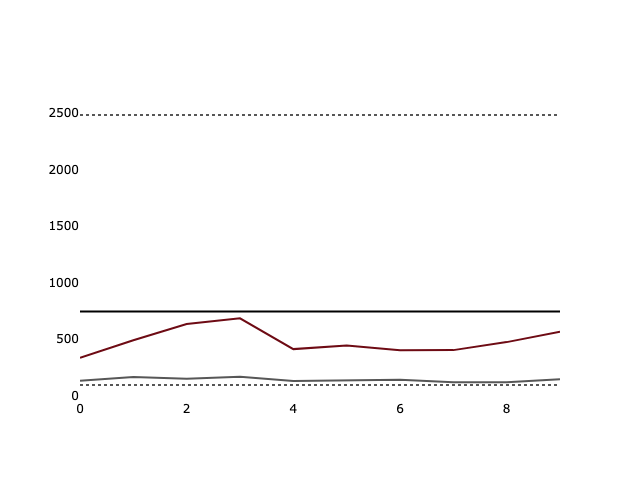
\includegraphics[width=\linewidth]{plots/prompt_1/prompt_1-command_r-cnn_dailymail/prompt_1-command_r-cnn_dailymail_t_word.png}
        \caption{Command-R+~\texttt{t\_word}\\CNN-DailyMail,~Scenario 1}\label{fig-command-r-t-word}
    \end{minipage}
    \hfill
    \begin{minipage}{0.32\textwidth}
        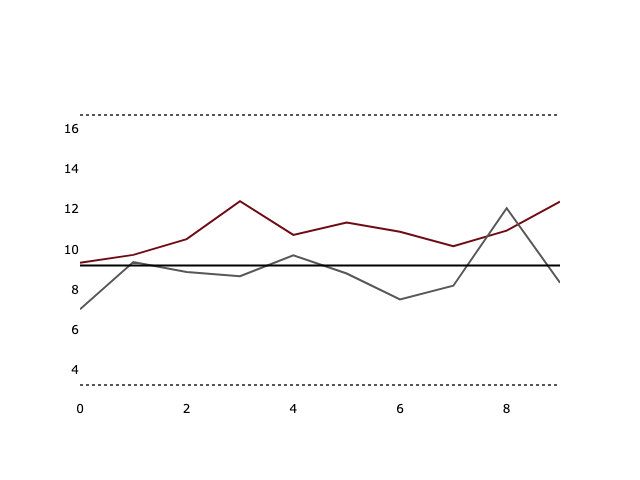
\includegraphics[width=\linewidth]{plots/prompt_1/prompt_1-gpt-cnn_dailymail/prompt_1-gpt-cnn_dailymail_fkgl.png}
        \caption{GPT~\texttt{fkgl}\\CNN-DailyMail,~Scenario 1}\label{fig-gpt-fkgl}
    \end{minipage}
    \hfill
    \begin{minipage}{0.32\textwidth}
        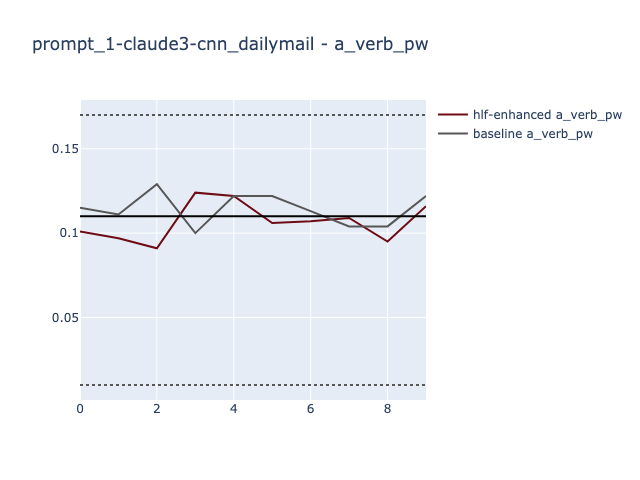
\includegraphics[width=\linewidth]{plots/prompt_1/prompt_1-claude3-cnn_dailymail/prompt_1-claude3-cnn_dailymail_a_verb_pw.png}
        \caption[center]{Claude3~\texttt{a\_verb\_pw}\\CNN-DailyMail,~Scenario 1}\label{fig-claude3-avpw}
    \end{minipage}
\end{figure*}

\subsection{HLF Instructions and Context Awareness}

The second scenario of our experiment uses examples to allow the LLM to
generate better baselines.
As pointed out at the end of Subsection~\ref{subsec:experiment-process}, we
assume that the difference we measure between baselines and HLF results is due
to the HLF instructions in the system prompt.

The first variant of the second scenario involves using input text from outside
the corpus.
Table~\ref{table-prompt-2-cnn-dailymail} contains the measurements we obtained
in this context.
We notice the HLF results tend to be closer to the target than the baseline
results.
In terms of significance and efficacy of the HLF instructions, the results are
similar to the ones obtained in the first scenario. 

\begin{table*}[ht!]
    \centering
    \resizebox{\textwidth}{!}{%
        \begin{tabular}{lllllllllll}
            model       & t\_word                      & t\_sent                    & n\_uverb                    & n\_uadj                    & simp\_ttr                 & a\_verb\_pw               & corr\_adj\_var            & corr\_verb\_var           & fkgl                       & a\_kup\_pw                \\
            \toprule
            claude3     & \textbf{\underline{718.49}}  & \textbf{\underline{24.13}} & \textbf{\underline{44.43}}  & \textbf{\underline{23.43}} & \textbf{\underline{0.4}}  & 0.03                      & 0.94                      & \textbf{\underline{0.77}} & 1.2                        & 0.07                      \\ \midrule
            gemini      & \textbf{\underline{785.6}}   & \textbf{\underline{25.8}}  & \textbf{\underline{60.5}}   & \textbf{\underline{41.6}}  & \textbf{\underline{0.41}} & \textbf{\underline{0.05}} & \textbf{\underline{1.95}} & \textbf{\underline{2.67}} & -4.62                      & \textbf{\textit{-1.94}}   \\ \midrule
            gpt         & 47.8                         & 5.18                       & 6.13                        & -0.13                      & 0.02                      & 0.0                       & 0.05                      & 0.3                       & 3.06                       & -0.27                     \\ \midrule
            command\_r  & \textbf{\underline{263.51}}  & 5.35                       & \textbf{\underline{25.08}}  & \textbf{\underline{17.37}} & \textbf{\textit{-0.09}}   & -0.01                     & \textbf{\underline{1.74}} & \textbf{\underline{1.42}} & \textbf{\underline{10.46}} & \textbf{\underline{1.56}} \\ \midrule
            llama3\_70b & \textbf{\underline{376.0}}   & \textbf{\underline{15.63}} & \textbf{\underline{38.63}}  & 15.74                      & \textbf{\underline{0.24}} & \textbf{\underline{0.06}} & 1.69                      & \textbf{\underline{2.91}} & 0.31                       & -0.3                      \\ \midrule
        \end{tabular}%
    }
    \caption{$Diff_N$ on the CNN-DailyMail corpus\\Scenario 2, Input Outside Corpus}\label{table-prompt-2-cnn-dailymail} % chktex-file 8
\end{table*}

We should note that there are fewer significant differences between baseline and
HLF results.
This seems to validate our assumption that using examples in the system prompt
causes the baselines to be closer to the target HLF value.

\begin{figure*}[ht!]
    \centering
    \begin{minipage}{0.32\textwidth}
        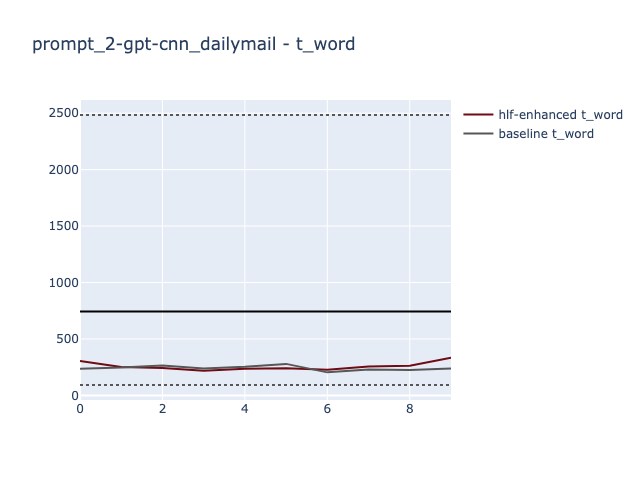
\includegraphics[width=\linewidth]{plots/prompt_2/prompt_2-gpt-cnn_dailymail/prompt_2-gpt-cnn_dailymail_t_word.png}
        \caption{GPT~\texttt{t\_word}\\CNN-DailyMail, Scenario 2, Input Outside Corpus}\label{fig-p2-gpt-twords}
    \end{minipage}
    \hfill
    \begin{minipage}{0.32\textwidth}
        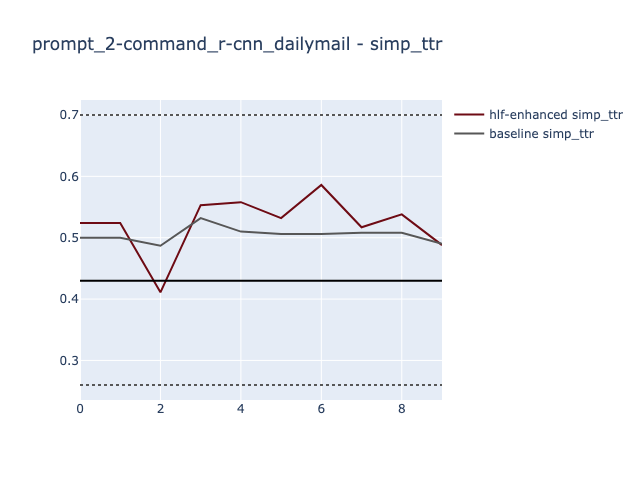
\includegraphics[width=\linewidth]{plots/prompt_2/prompt_2-command_r-cnn_dailymail/prompt_2-command_r-cnn_dailymail_simp_ttr.png}
        \caption{Command-R+~\texttt{simp\_ttr}\\CNN-DailyMail, Scenario 2, Input Outside Corpus}\label{fig-p2-command-r-simpttr}
    \end{minipage}
    \hfill
    \begin{minipage}{0.32\textwidth}
        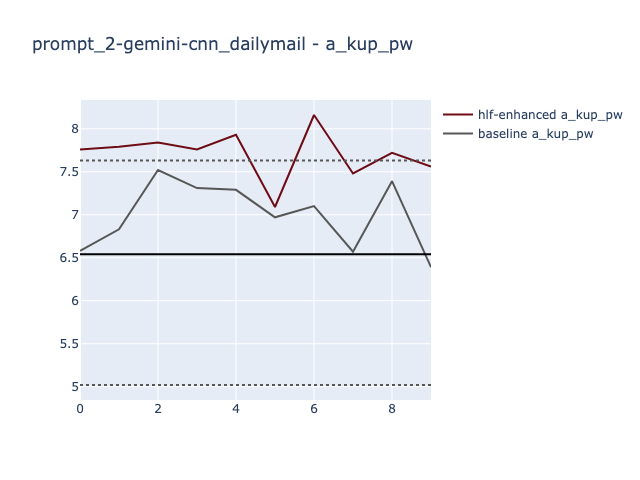
\includegraphics[width=\linewidth]{plots/prompt_2/prompt_2-gemini-cnn_dailymail/prompt_2-gemini-cnn_dailymail_a_kup_pw.png}
        \caption[center]{Gemini~\texttt{a\_kup\_pw}\\CNN-DailyMail, Scenario 2, Input Outside Corpus}\label{fig-p2-gemini-a-kup-pw}
    \end{minipage}
\end{figure*}

There are exceptions to the general trend observed for the first scenario.
One such exception is highlighted in Figure~\ref{fig-p2-gpt-twords}.
In~\cref{fig-p2-command-r-simpttr,fig-p2-gemini-a-kup-pw} we even observe
regressions in performance with significant differences between baseline and
result.
Even so, these are exceptions and the results obtained in our first scenario are
largely confirmed.

Finally, the second variant of the second scenario investigates the suggestion
power of HLF instructions.
By using input from the corpus, the LLM should produce baselines that comply
even more to the target HLFs statistics computed on the corpus.
We expect fewer significant differences between baselines and HLF results.
Additionally, HLF results should be closer to the target than in our previous
observations.

\begin{table*}[ht]
    \centering
    \resizebox{\textwidth}{!}{%
        \begin{tabular}{lllllllllll}
            model       & t\_word                      & t\_sent                     & n\_uverb                    & n\_uadj                    & simp\_ttr                 & a\_verb\_pw               & corr\_adj\_var             & corr\_verb\_var            & fkgl                       & a\_kup\_pw              \\
            \toprule
            claude3     & \textbf{\underline{871.02}}  & \textbf{\underline{34.2}}   & \textbf{\underline{34.48}}  & \textbf{\textit{-7.38}}    & \textbf{\underline{0.27}} & 0.01                      & \textbf{\textit{-0.93}}    & \textbf{\textit{-0.72}}    & 1.16                       & -0.14                   \\ \midrule
            gemini      & \textbf{\underline{1315.41}} & \textbf{\underline{46.19}}  & \textbf{\underline{114.47}} & \textbf{\underline{72.38}} & \textbf{\underline{1.17}} & 0.03                      & \textbf{\underline{5.25}}  & \textbf{\underline{6.64}}  & -1.6                       & \textbf{\textit{-2.1}}  \\ \midrule
            gpt         & \textbf{\underline{521.29}}  & \textbf{\underline{23.3}}   & \textbf{\underline{43.13}}  & 19.85                      & \textbf{\underline{0.2}}  & 0.02                      & 1.08                       & \textbf{\underline{1.04}}  & 5.09                       & 0.67                    \\ \midrule
            command\_r  & \textbf{\underline{371.08}}  & \textbf{\underline{13.31}}  & 22.06                       & \textbf{\underline{17.19}} & \textbf{\underline{0.17}} & \textbf{\underline{0.02}} & 0.88                       & 1.09                       & \textbf{\underline{4.05}}  & -0.15                   \\ \midrule
            llama3\_70b & \textbf{\underline{1040.85}} & \textbf{\underline{41.99}}  & \textbf{\underline{80.58}}  & \textbf{\underline{49.12}} & \textbf{\underline{0.55}} & \textbf{\underline{0.04}} & \textbf{\underline{3.99}}  & \textbf{\underline{5.05}}  & 7.18                       & \textbf{\textit{-1.94}} \\ \midrule
        \end{tabular}%
    }
    \caption{$Diff_N$ on CNN-DailyMail\\Scenario 2, Input Inside Corpus}\label{table-prompt-2-ifd-cnn-dailymail}
\end{table*}

The results shown in Table~\ref{table-prompt-2-ifd-cnn-dailymail} contradict
these expectations.
The most surprising behaviour is exhibited for HLFs which are derived into more
concrete generation instructions, such as the total number of
words~(Figure~\ref{fig-p2-ifd-gemini-twords}).
Additionally, we notice regressive behaviour for some models compared to the
previously explored results in Figure~\ref{fig-p2-ifd-claude3-nuadj}.
Finally, notice that the abstractness of the text generation instructions for
certain HLFs leads to non-compliance in Figure~\ref{fig-p2-ifd-llama3-a-kup-pw}.

\begin{figure*}[ht!]
    \centering
    \begin{minipage}{0.32\textwidth}
        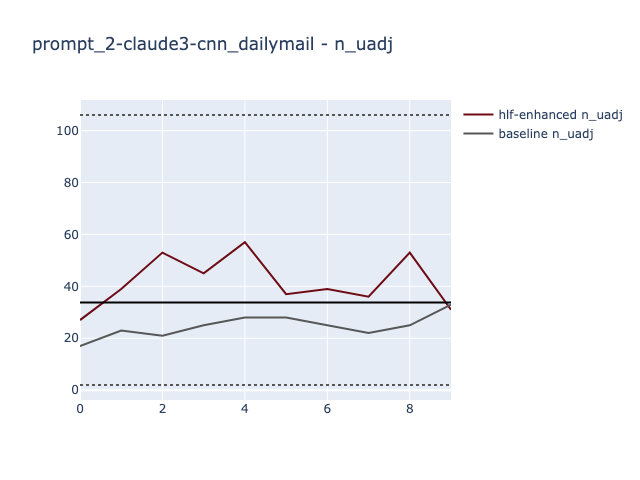
\includegraphics[width=\linewidth]{plots/prompt_2_ifd/prompt_2-claude3-cnn_dailymail/prompt_2-claude3-cnn_dailymail_n_uadj.png}
        \caption{Claude3\texttt{n\_uadj}\\CNN-DailyMail, Scenario 2, Input Inside Corpus}\label{fig-p2-ifd-claude3-nuadj}
    \end{minipage}
    \hfill
    \begin{minipage}{0.32\textwidth}
        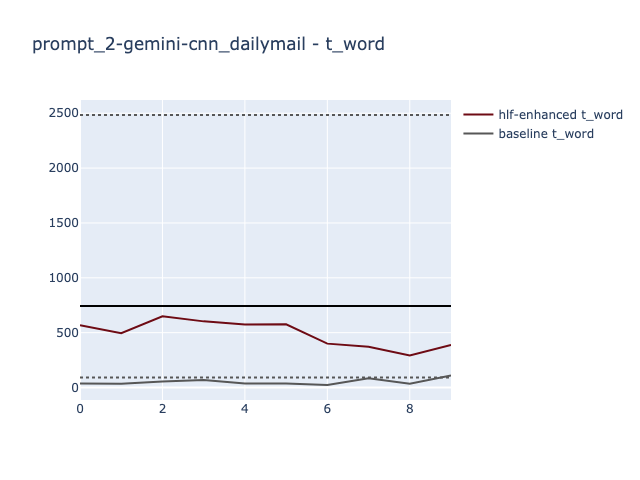
\includegraphics[width=\linewidth]{plots/prompt_2_ifd/prompt_2-gemini-cnn_dailymail/prompt_2-gemini-cnn_dailymail_t_word.png}
        \caption{Gemini\texttt{t\_word}\\CNN-DailyMail, Scenario 2, Input Inside Corpus}\label{fig-p2-ifd-gemini-twords}
    \end{minipage}
    \hfill
    \begin{minipage}{0.32\textwidth}
        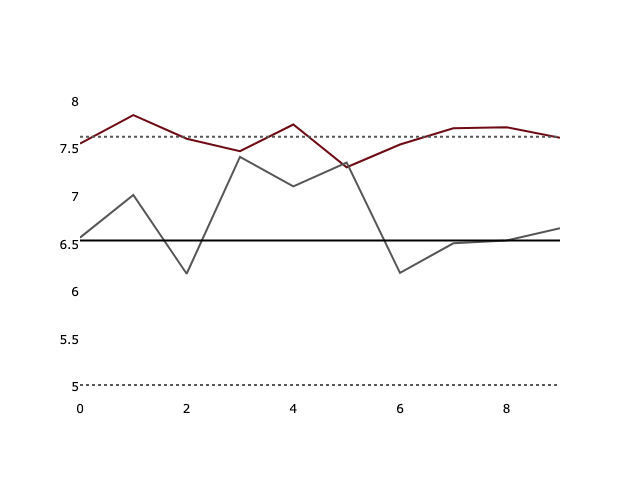
\includegraphics[width=\linewidth]{plots/prompt_2_ifd/prompt_2-llama3_70b-cnn_dailymail/prompt_2-llama3_70b-cnn_dailymail_a_kup_pw.png}
        \caption[center]{Llama3\texttt{a\_kup\_pw}\\CNN-DailyMail, Scenario 2, Input Inside Corpus}\label{fig-p2-ifd-llama3-a-kup-pw}
    \end{minipage}
\end{figure*}

The overall sentiment, taking into account the additional results obtained on
the Yelp dataset, is that LLMs do \textit{not} take advantage of the examples
from text corpora for the tasks performed in this experiment.

\section{Discussion}

In terms of our first question --- whether HLF instructions impact an LLM's
writing, the response is affirmative.
Not all LLMs are equally susceptible to HLF instructions, though.
The experiment design involves choices that rely on the presence of a corpus and
the usage of a fixed external input text.
This is relevant as evidentiated by the difference in HLF results obtained using
the Yelp reviews corpus when compared to the HLF results obtained on the CNN
article corpus.
While similarly significant, the HLF results on Yelp reviews are mostly worse
than their corresponding baselines failing to confirm the positive impact of HLF
instructions.
The importance of the choice of the external text is highlighted by the better
HLF results obtained using an input text from the corpus.

There is more doubt in response to how much HLF instructions impact an LLM's
writing.
The metrics we compute dismiss the idea that HLF instructions have a consistent
desired impact on the generated text.
There isn't conclusive evidence that if we improve the LLM's chances of
producing a better baseline, this will result in a smaller difference between
baseline and HLF result relative to the target HLF.
In fact, there is evidence that HLF instructions have an adverse effect when
examining the HLF results obtained on the Yelp reviews dataset.
This is especially true of highly abstract HLF instructions.
LLMs do not seem to follow these instructions well in most scenarios.

The choice of input text in relation to the target HLF values is consequential.
LLMs don't yet seem able to cover the gulf between Oscar Wilde poems and the
average Yelp review in terms of linguistic features.
We surmise that even if LLMs are able to generate text that complies to certain
target HLFs, there is a limit to this ability.

\section{Limitations and Future Work}

Other experiments are required to better understand the capabilities of large
language models with regard to HLFs.
The selection of language models, the reliance on a corpus for computing target
linguistic features, the fixed choice of input text and not least of all the
wording of the system prompts are all limitations of the current approach.

Making different experiment design choices in all these respects might yield
more positive and more powerful results.
Using a selection of HLFs and not individually analysing the behaviour of the
LLM under the influence of each individual HLF is another limiting choice that
invites to future work on the alternative.

\section{Conclusions}

We designed an experiment that tries to understand whether it is possible to
generate text that exhibits certain linguistic features by instructing a large
language model.
It turns out state of the art large language models are receptive to
instructions regarding the linguistic features of the output.
This is especially true for concrete instructions.

However, the outcomes are not always good.
From a pragmatic standpoint, prompt engineering and a careful choice of language
features and input text seem like the way to obtain desirable results.
Providing examples in the input prompt does not seem to influence the HLFs of
the LLM output in the expected manner.
Rewording text which already exhibits the desired linguistic features can have
adverse effects, too.

Finally, we've seen how we might use handcrafted linguistic features to assess
LLM output.
Setting up ``before and after'' scenarios to evaluate relative improvements of
the LLM outcome in relation to the selected HLFs is one way to achieve this.
With enough measurements, the relative difference between baselines and target
HLFs can be quantified using geometric or statistical means.

\bibliography{references}

\appendix

\section{Additional Result Tables}\label{sec:yelp-tables}
\subsection{Yelp}
\Cref{table-prompt-1-yelp,table-prompt-2-yelp,table-prompt-2-ifd-yelp} show the
experiment results on the corpus of reviews extracted from the Yelp dataset.

\begin{table*}[ht]
    \centering
    \resizebox{\textwidth}{!}{%
        \begin{tabular}{lllllllllll}
            model                 & t\_word                   & t\_sent                    & n\_uverb                 & n\_uadj                  & simp\_ttr & a\_verb\_pw             & corr\_adj\_var          & corr\_verb\_var         & fkgl                       & a\_kup\_pw               \\
            \toprule
            claude3 $Diff_N$     & \textbf{\textit{-281.9}}  & \textbf{\textit{-13.22}}   & \textbf{\textit{-25.79}} & -14.56                   & -0.06     & 0.0                     & -1.27                   & -1.14                   & \textbf{\underline{6.89}}  & \textbf{\underline{1.0}} \\ \midrule
            claude3 $Diff_A$     & \textbf{\textit{-774.0}}  & \textbf{\textit{-27.76}}   & \textbf{\textit{-70.0}}  & -38.0                    & -0.19     & 0.02                    & -3.25                   & -3.39                   & \textbf{\underline{21.68}} & \textbf{\underline{2.9}} \\ \midrule
            gemini $Diff_N$      & -109.27                   & 0.05                       & -7.25                    & -13.18                   & -0.14     & 0.01                    & -1.01                   & -0.4                    & 1.62                       & -0.4                     \\ \midrule
            gemini $Diff_A$      & -252.82                   & -0.78                      & -17.5                    & -23.14                   & -0.52     & 0.01                    & -1.85                   & -1.07                   & 7.14                       & -0.93                    \\ \midrule
            gpt $Diff_N$         & -21.62                    & 2.42                       & -3.8                     & -8.84                    & 0.0       & -0.01                   & -0.8                    & -0.53                   & 8.94                       & -0.37                    \\ \midrule
            gpt $Diff_A$         & -34.72                    & 9.68                       & -10.54                   & -24.57                   & -0.03     & -0.02                   & -2.37                   & -1.58                   & 19.26                      & -1.03                    \\ \midrule
            command\_r $Diff_N$  & -40.1                     & 1.22                       & 2.43                     & \textbf{\textit{-13.64}} & 0.05      & \textbf{\textit{-0.04}} & \textbf{\textit{-1.17}} & 0.59                    & \textbf{\textit{-7.25}}    & \textbf{\textit{-1.67}}  \\ \midrule
            command\_r $Diff_A$  & -75.5                     & 1.5                        & 12.94                    & \textbf{\textit{-34.0}}  & 0.19      & \textbf{\textit{-0.12}} & \textbf{\textit{-2.76}} & 2.83                    & \textbf{\textit{-20.49}}   & \textbf{\textit{-4.76}}  \\ \midrule
            llama3\_70b $Diff_N$ & \textbf{\textit{-210.45}} & \textbf{\underline{6.87}}  & \textbf{\textit{-13.46}} & \textbf{\textit{-15.17}} & -0.16     & \textbf{\textit{-0.02}} & \textbf{\textit{-1.78}} & \textbf{\textit{-1.31}} & 3.7                        & \textbf{\textit{-1.58}}  \\ \midrule
            llama3\_70b $Diff_A$ & \textbf{\textit{-607.52}} & \textbf{\underline{19.42}} & \textbf{\textit{-41.22}} & \textbf{\textit{-44.77}} & -0.42     & \textbf{\textit{-0.05}} & \textbf{\textit{-5.48}} & \textbf{\textit{-4.34}} & 9.79                       & \textbf{\textit{-4.98}}  \\ \bottomrule
        \end{tabular}%
    }
    \caption{Yelp Results - Prompt Without Examples}\label{table-prompt-1-yelp} % chktex-file 8
\end{table*}

\begin{table*}[!ht]
    \centering
    \resizebox{\textwidth}{!}{%
        \begin{tabular}{lllllllllll}
            model                 & t\_word & t\_sent & n\_uverb & n\_uadj & simp\_ttr & a\_verb\_pw & corr\_adj\_var            & corr\_verb\_var & fkgl                       & a\_kup\_pw \\
            \toprule
            claude3 $Diff_N$     & -121.77 & -4.61   & -9.9     & 18.41   & -0.11     & 0.03        & \textbf{\underline{1.4}}  & -0.33           & 1.81                       & 0.95       \\ \midrule
            claude3 $Diff_A$     & -394.5  & -11.5   & -37.5    & 60.0    & -0.37     & 0.09        & \textbf{\underline{4.66}} & -1.49           & 5.38                       & 2.62       \\ \midrule
            gemini $Diff_N$      & -23.49  & 1.52    & -0.55    & -1.29   & -0.02     & -0.01       & 0.09                      & -0.05           & \textbf{\underline{6.41}}  & 0.2        \\ \midrule
            gemini $Diff_A$      & -83.0   & 3.0     & -2.5     & -6.36   & -0.0      & -0.03       & 0.26                      & -0.08           & \textbf{\underline{19.63}} & 0.53       \\ \midrule
            gpt $Diff_N$         & 13.66   & 2.83    & -3.65    & -3.19   & 0.04      & -0.04       & -0.24                     & -0.22           & 7.5                        & 0.0        \\ \midrule
            gpt $Diff_A$         & 55.5    & 9.5     & -9.86    & -12.86  & 0.14      & -0.11       & -0.84                     & -0.22           & 18.67                      & -0.38      \\ \midrule
            command\_r $Diff_N$  & -188.71 & 0.69    & -10.73   & 1.17    & -0.23     & -0.01       & \textbf{\underline{0.74}} & -0.83           & \textbf{\textit{-5.02}}    & -0.08      \\ \midrule
            command\_r $Diff_A$  & -516.82 & 2.02    & -29.22   & 8.28    & -0.66     & -0.0        & \textbf{\underline{2.98}} & -2.48           & \textbf{\textit{-14.52}}   & -0.48      \\ \midrule
            llama3\_70b $Diff_N$ & -202.95 & -7.84   & -13.73   & 1.43    & -0.15     & -0.04       & 0.38                      & -1.39           & 10.67                      & 1.37       \\ \midrule
            llama3\_70b $Diff_A$ & -561.24 & -18.78  & -49.94   & 5.07    & -0.38     & -0.14       & 1.62                      & -4.81           & 29.26                      & 3.11       \\ \bottomrule
        \end{tabular}%
    }
    \caption{Yelp Results - Prompt With Examples\\Input External To Corpus}\label{table-prompt-2-yelp}
\end{table*}
\begin{table*}[!ht]
    \centering
    \resizebox{\textwidth}{!}{%
        \begin{tabular}{lllllllllll}
            model                 & t\_word                   & t\_sent                 & n\_uverb                  & n\_uadj                  & simp\_ttr               & a\_verb\_pw & corr\_adj\_var          & corr\_verb\_var         & fkgl                    & a\_kup\_pw              \\
            \toprule
            claude3 $Diff_N$     & -148.13                   & -1.63                   & -3.93                     & \textbf{\textit{-46.03}} & -0.11                   & -0.0        & \textbf{\textit{-3.08}} & -0.31                   & -4.3                    & \textbf{\textit{-1.53}} \\ \midrule
            claude3 $Diff_A$     & -526.14                   & -7.98                   & -23.86                    & \textbf{\textit{-133.5}} & -0.41                   & -0.0        & \textbf{\textit{-8.98}} & -1.75                   & -21.03                  & \textbf{\textit{-5.34}} \\ \midrule
            gemini $Diff_N$      & 74.27                     & 0.65                    & 4.67                      & 2.98                     & 0.04                    & -0.0        & -0.22                   & 1.05                    & 1.44                    & -0.65                   \\ \midrule
            gemini $Diff_A$      & 221.0                     & 2.0                     & 10.5                      & 7.44                     & 0.12                    & -0.03       & -0.85                   & 2.73                    & 3.28                    & -1.79                   \\ \midrule
            gpt $Diff_N$         & 0.65                      & 4.03                    & -1.19                     & -2.66                    & -0.03                   & -0.01       & -0.17                   & -0.13                   & 1.05                    & -0.67                   \\ \midrule
            gpt $Diff_A$         & 17.0                      & 11.68                   & -3.68                     & -7.0                     & -0.1                    & -0.04       & -0.43                   & -0.05                   & 0.57                    & -1.75                   \\ \midrule
            command\_r $Diff_N$  & \textbf{\textit{-236.11}} & \textbf{\textit{-3.6}}  & \textbf{\textit{-0.97}}   & \textbf{\textit{-27.04}} & \textbf{\textit{-0.23}} & 0.0         & -1.24                   & \textbf{\textit{-1.08}} & \textbf{\textit{-2.13}} & \textbf{\textit{-1.09}} \\ \midrule
            command\_r $Diff_A$  & \textbf{\textit{-727.0}}  & \textbf{\textit{-9.24}} & \textbf{\underline{0.76}} & \textbf{\textit{-68.5}}  & \textbf{\textit{-0.64}} & 0.02        & -2.89                   & \textbf{\textit{-3.08}} & \textbf{\textit{-5.5}}  & \textbf{\textit{-3.0}}  \\ \midrule
            llama3\_70b $Diff_N$ & \textbf{\textit{-333.03}} & \textbf{\textit{-5.19}} & 4.43                      & \textbf{\textit{-21.38}} & -0.16                   & -0.03       & \textbf{\textit{-1.77}} & -0.03                   & 1.87                    & -0.44                   \\ \midrule
            llama3\_70b $Diff_A$ & \textbf{\textit{-687.34}} & \textbf{\textit{-3.42}} & 10.7                      & \textbf{\textit{-61.64}} & -0.31                   & -0.04       & \textbf{\textit{-5.6}}  & -0.89                   & 3.0                     & -1.92                   \\ \bottomrule
        \end{tabular}%
    }
    \caption{Yelp Results - Prompt With Examples\\Input From Corpus}\label{table-prompt-2-ifd-yelp}
\end{table*}

\section{Additional Plots}

\subsection{GPT}

\begin{figure*}[ht]
    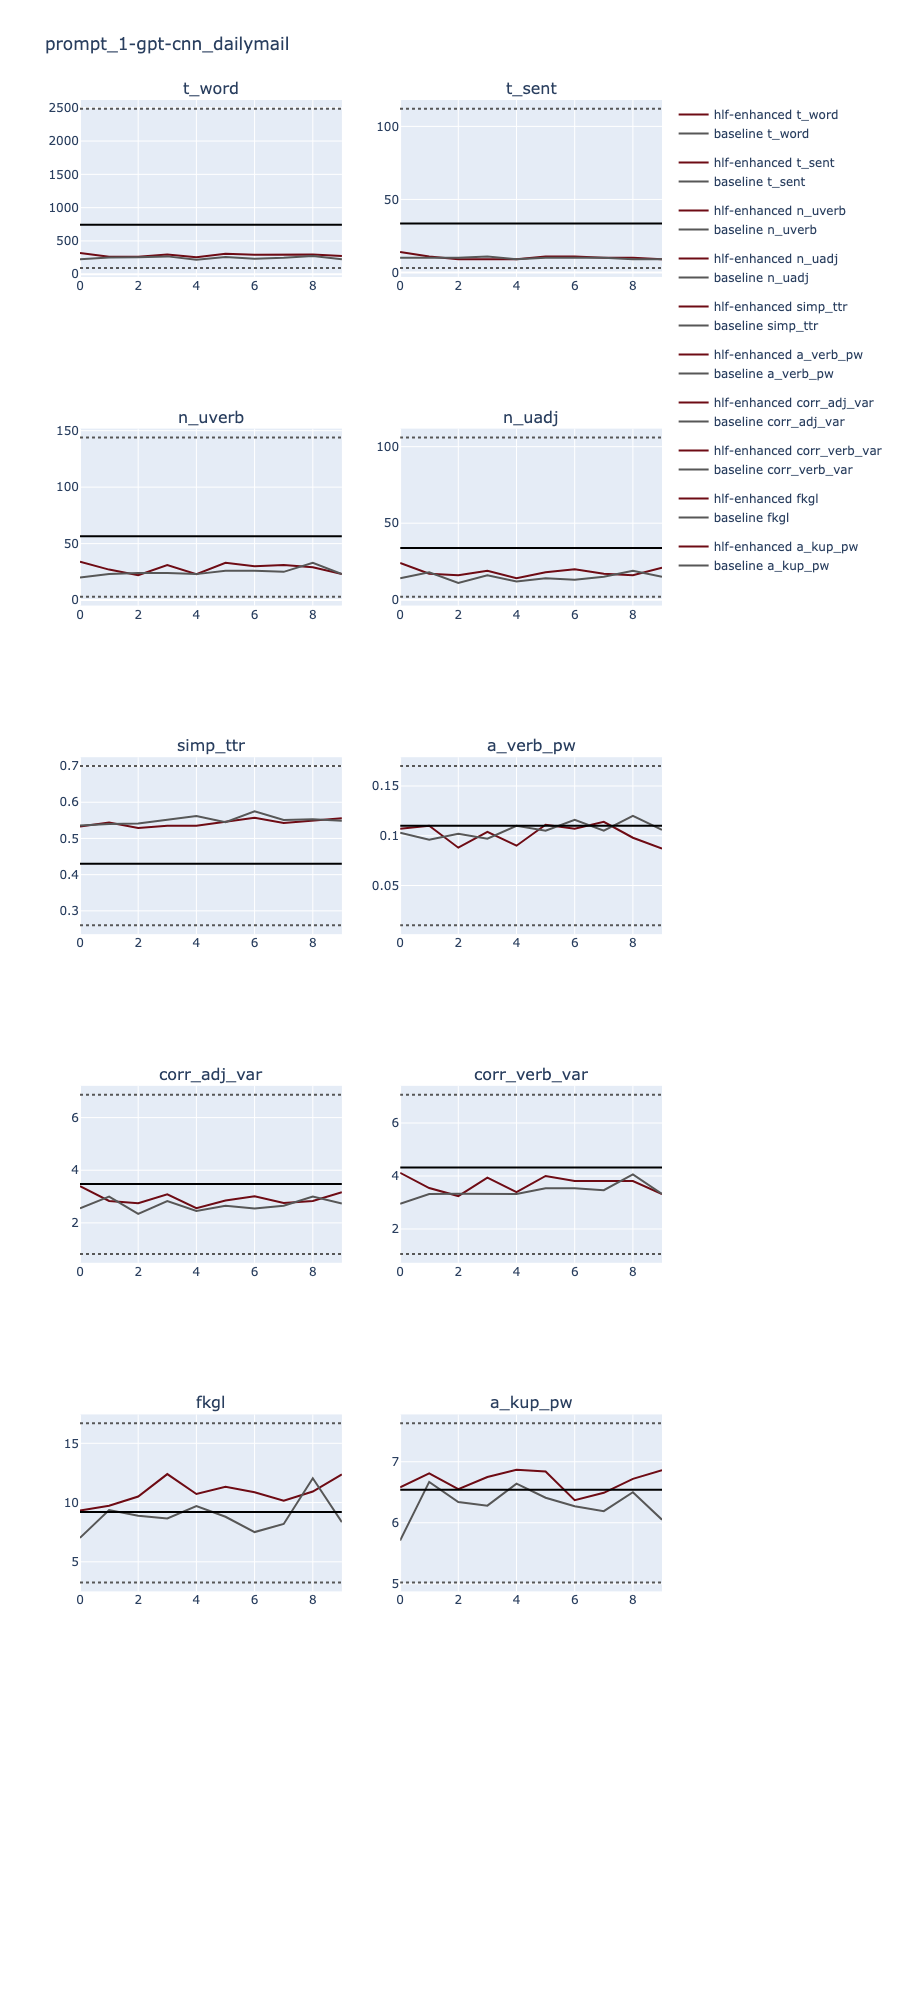
\includegraphics[width=\textwidth,height=0.9\textheight,scale=1]{plots/prompt_1/prompt_1-gpt-cnn_dailymail/prompt_1-gpt-cnn_dailymail.png}
    \caption{GPT on CNN Corpus\\Prompt Without Examples}\label{fig:gpt-prompt1-cnn}
\end{figure*}
\begin{figure*}[ht]
    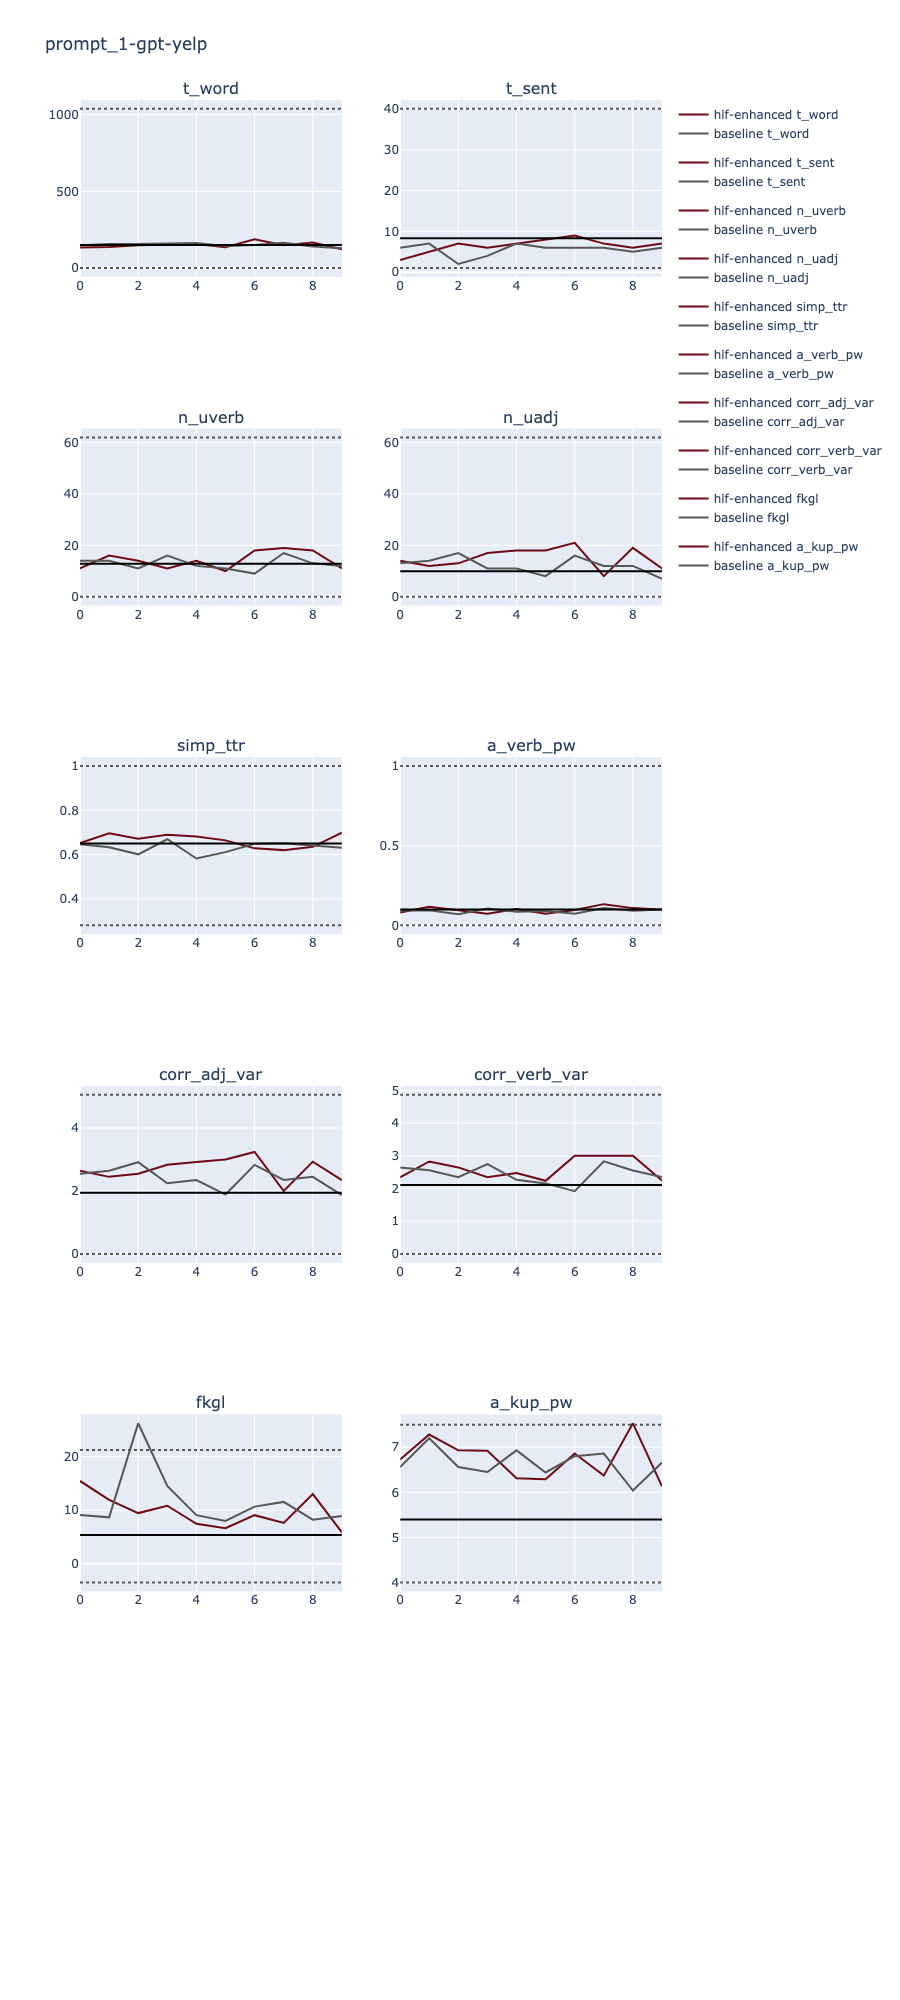
\includegraphics[width=\textwidth,height=0.9\textheight,scale=1]{plots/prompt_1/prompt_1-gpt-yelp/prompt_1-gpt-yelp.png}
    \caption{GPT on Yelp Corpus\\Prompt Without Examples}\label{fig:gpt-prompt1-yelp}
\end{figure*}
\begin{figure*}[ht]
    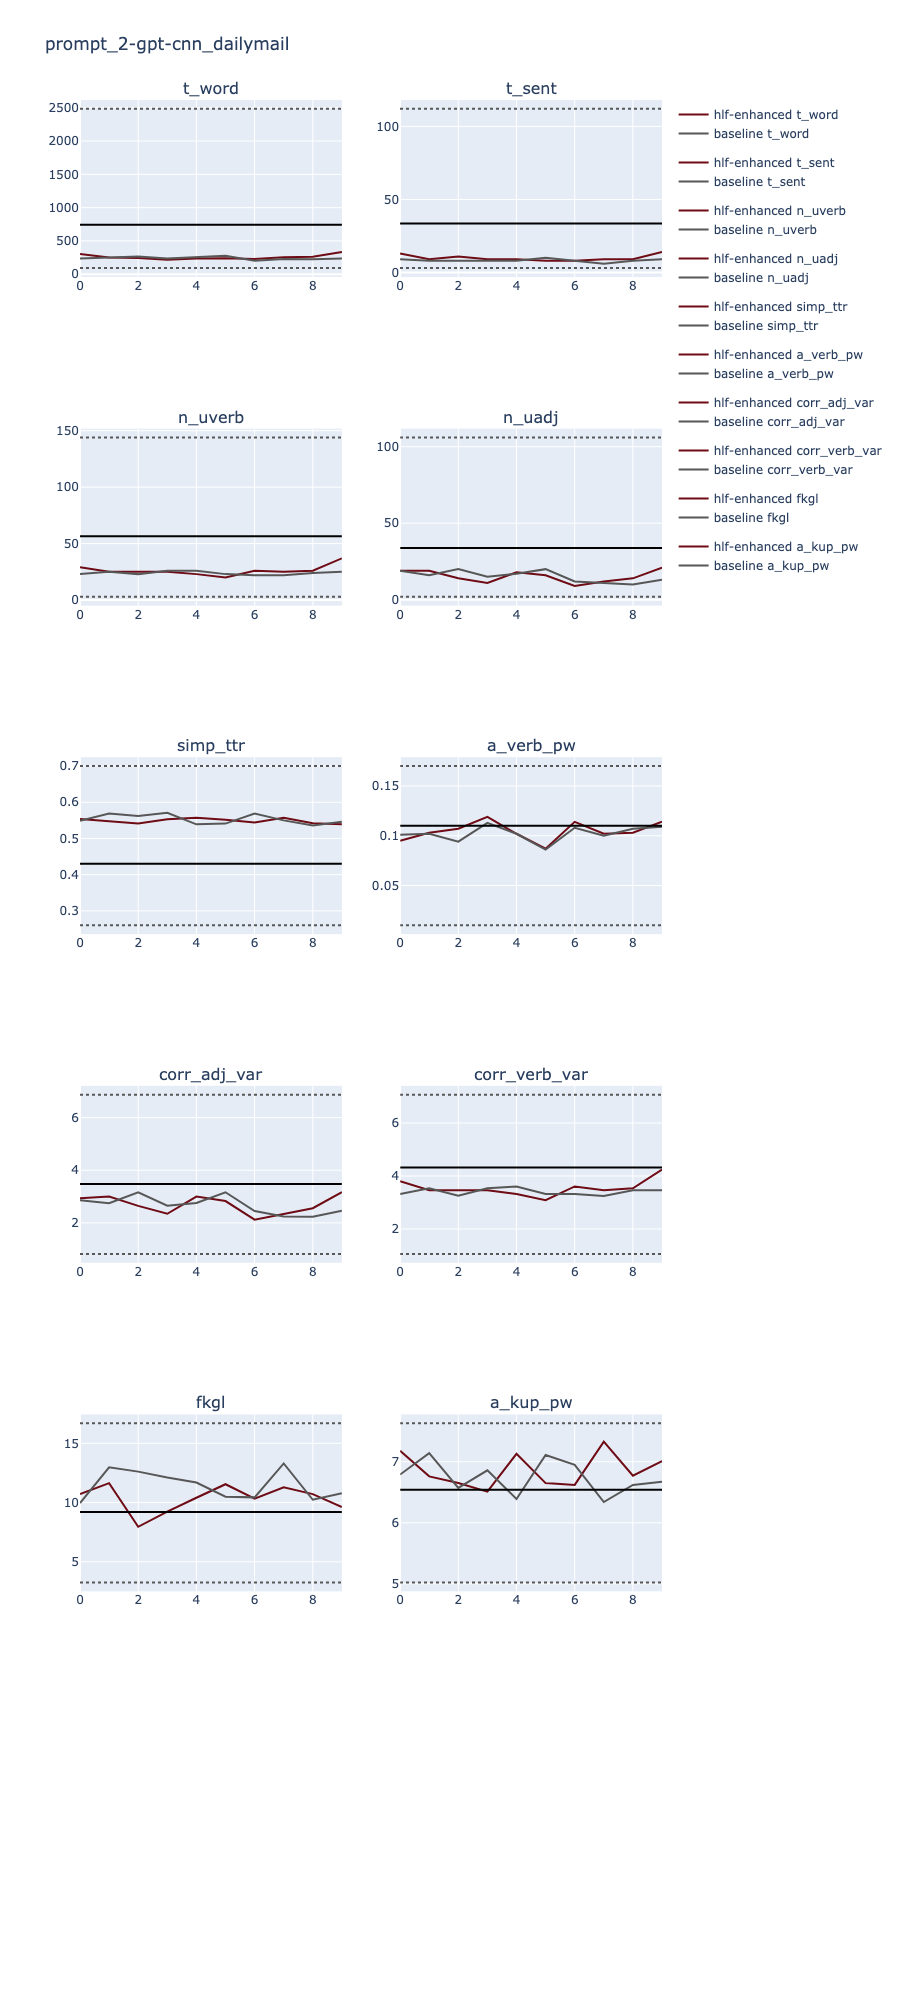
\includegraphics[width=\textwidth,height=0.9\textheight,scale=1]{plots/prompt_2/prompt_2-gpt-cnn_dailymail/prompt_2-gpt-cnn_dailymail.png}
    \caption{GPT on CNN Corpus\\Prompt With Examples\\Extraneous Input}\label{fig:gpt-prompt2-cnn}
\end{figure*}
\begin{figure*}[ht]
    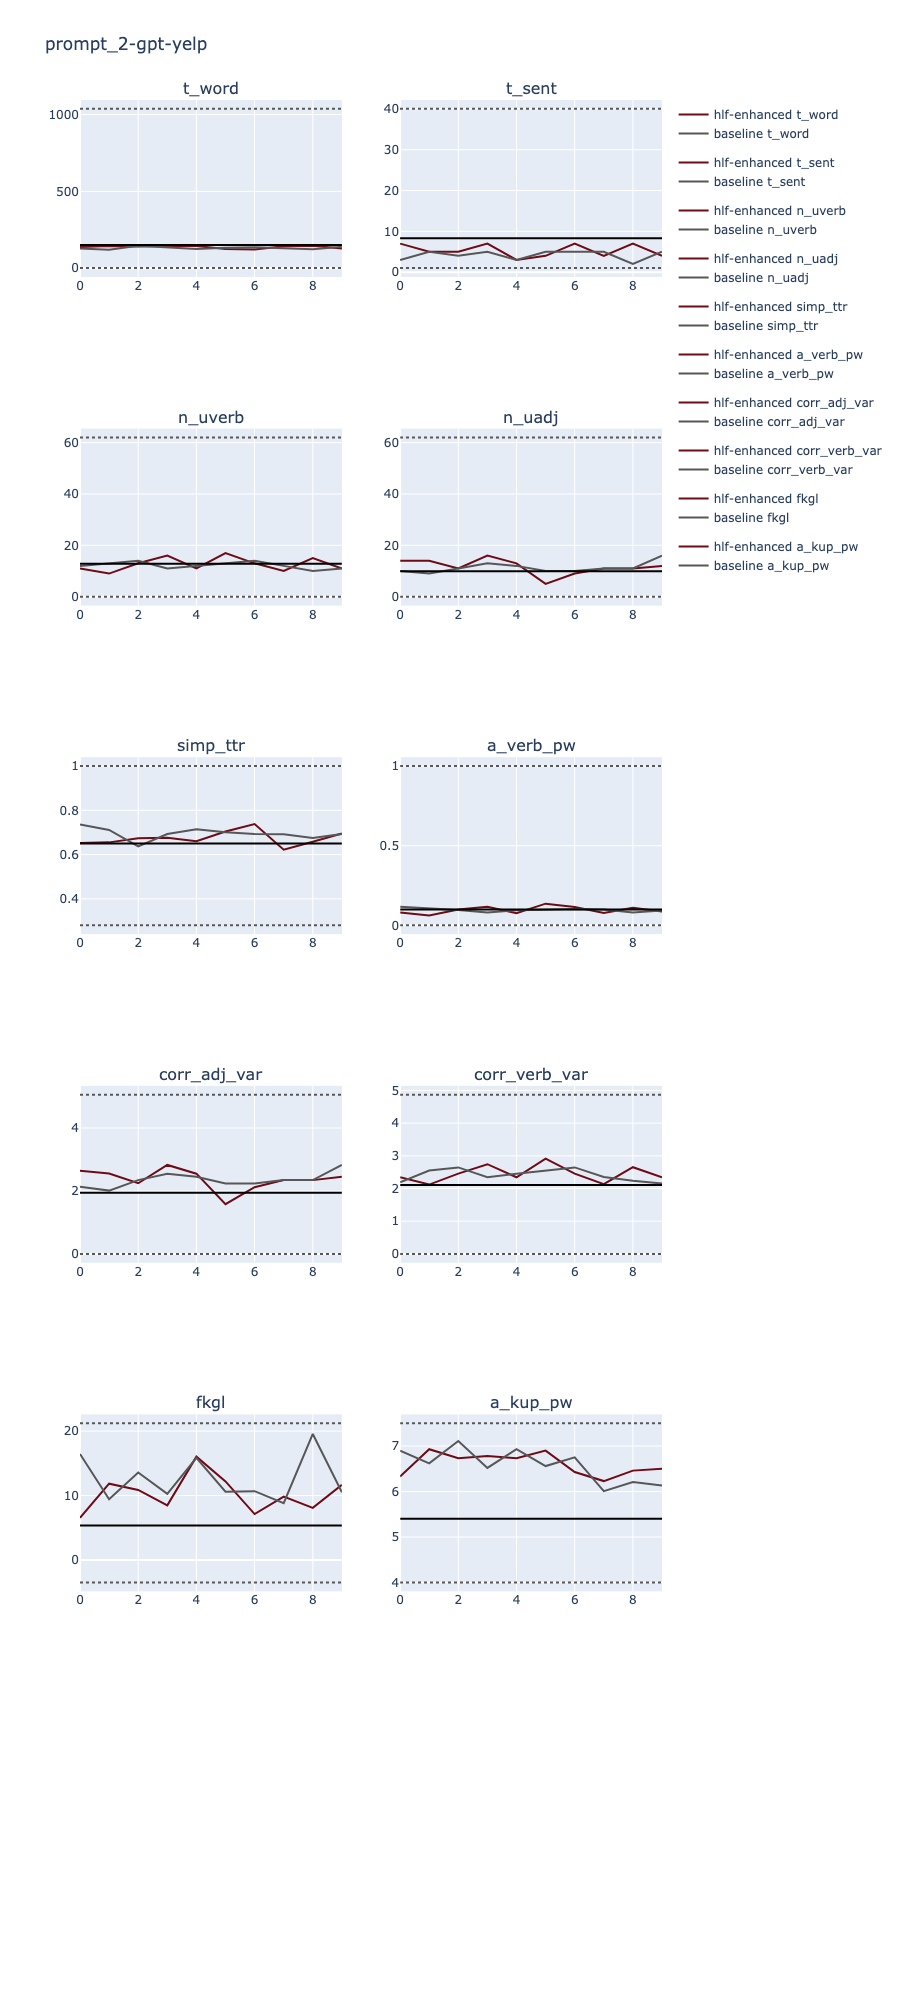
\includegraphics[width=\textwidth,height=0.9\textheight,scale=1]{plots/prompt_2/prompt_2-gpt-yelp/prompt_2-gpt-yelp.png}
    \caption{GPT on Yelp Corpus\\Prompt With Examples\\Extraneous Input}\label{fig:gpt-prompt2-yelp}
\end{figure*}
\begin{figure*}[ht]
    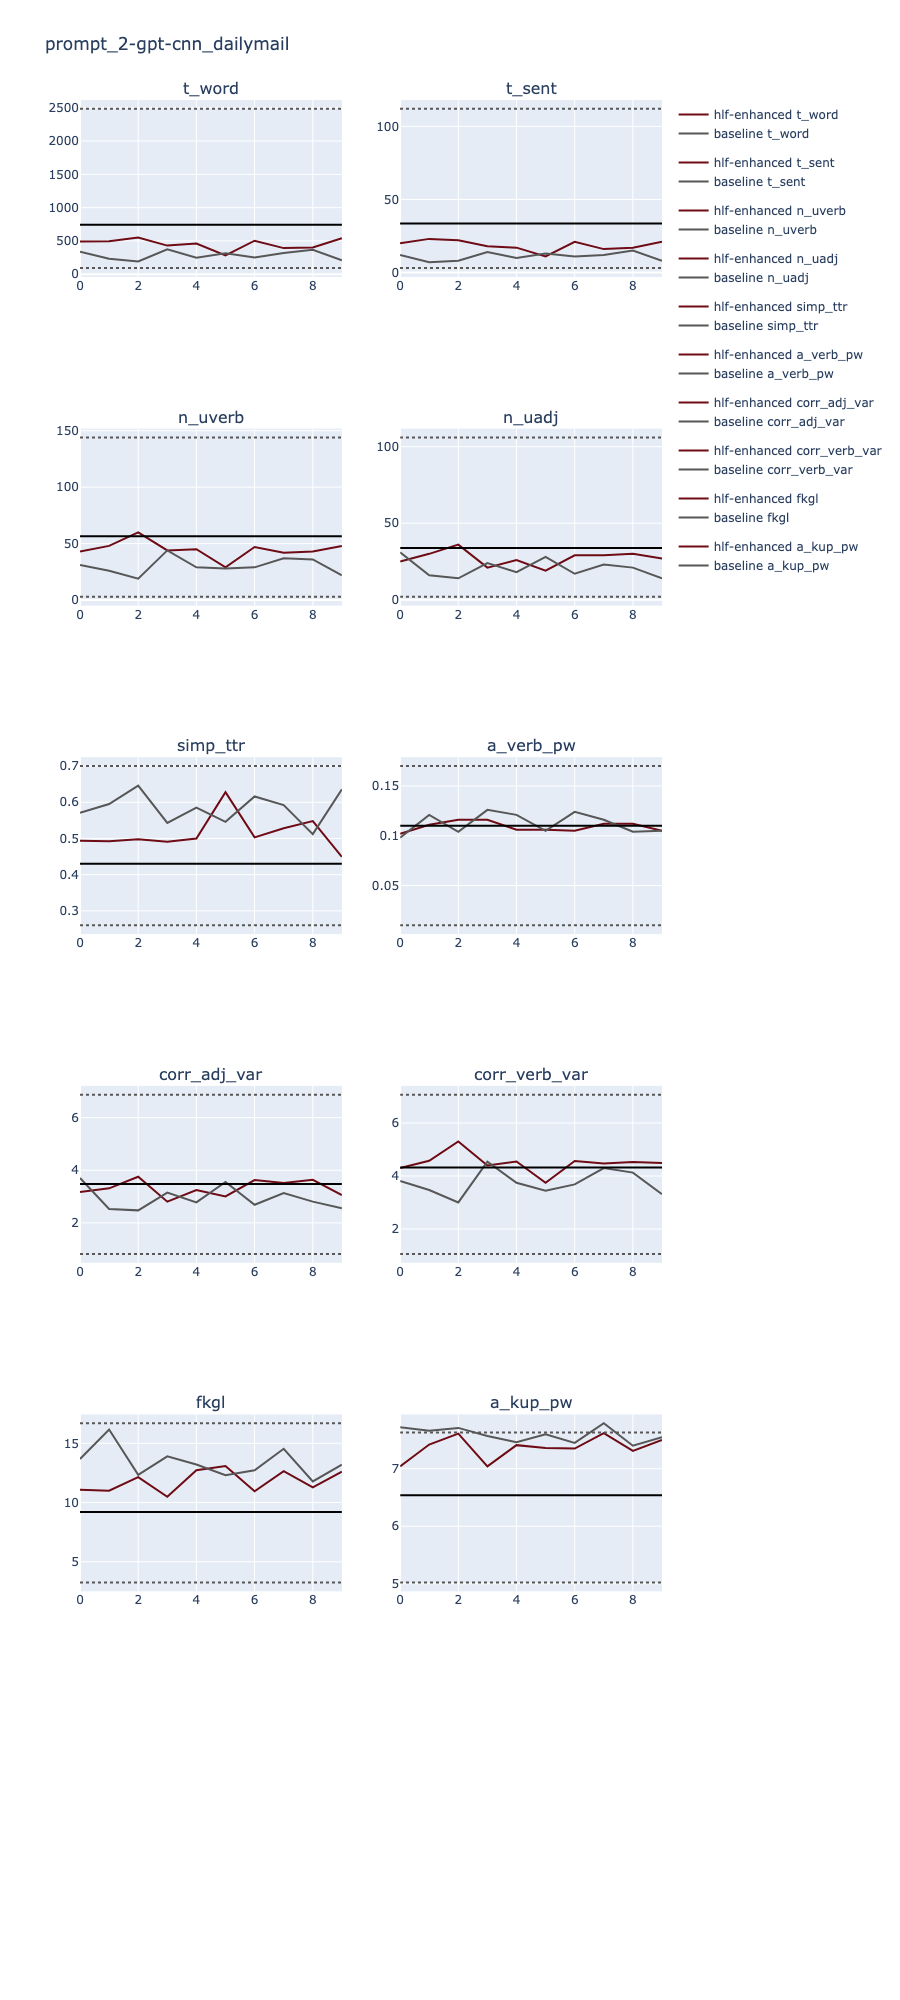
\includegraphics[width=\textwidth,height=0.9\textheight,scale=1]{plots/prompt_2_ifd/prompt_2-gpt-cnn_dailymail/prompt_2-gpt-cnn_dailymail.png}
    \caption{GPT on CNN Corpus\\Prompt With Examples\\Input from Corpus}\label{fig:gpt-prompt2-cnn-ifd}
\end{figure*}
\begin{figure*}[ht]
    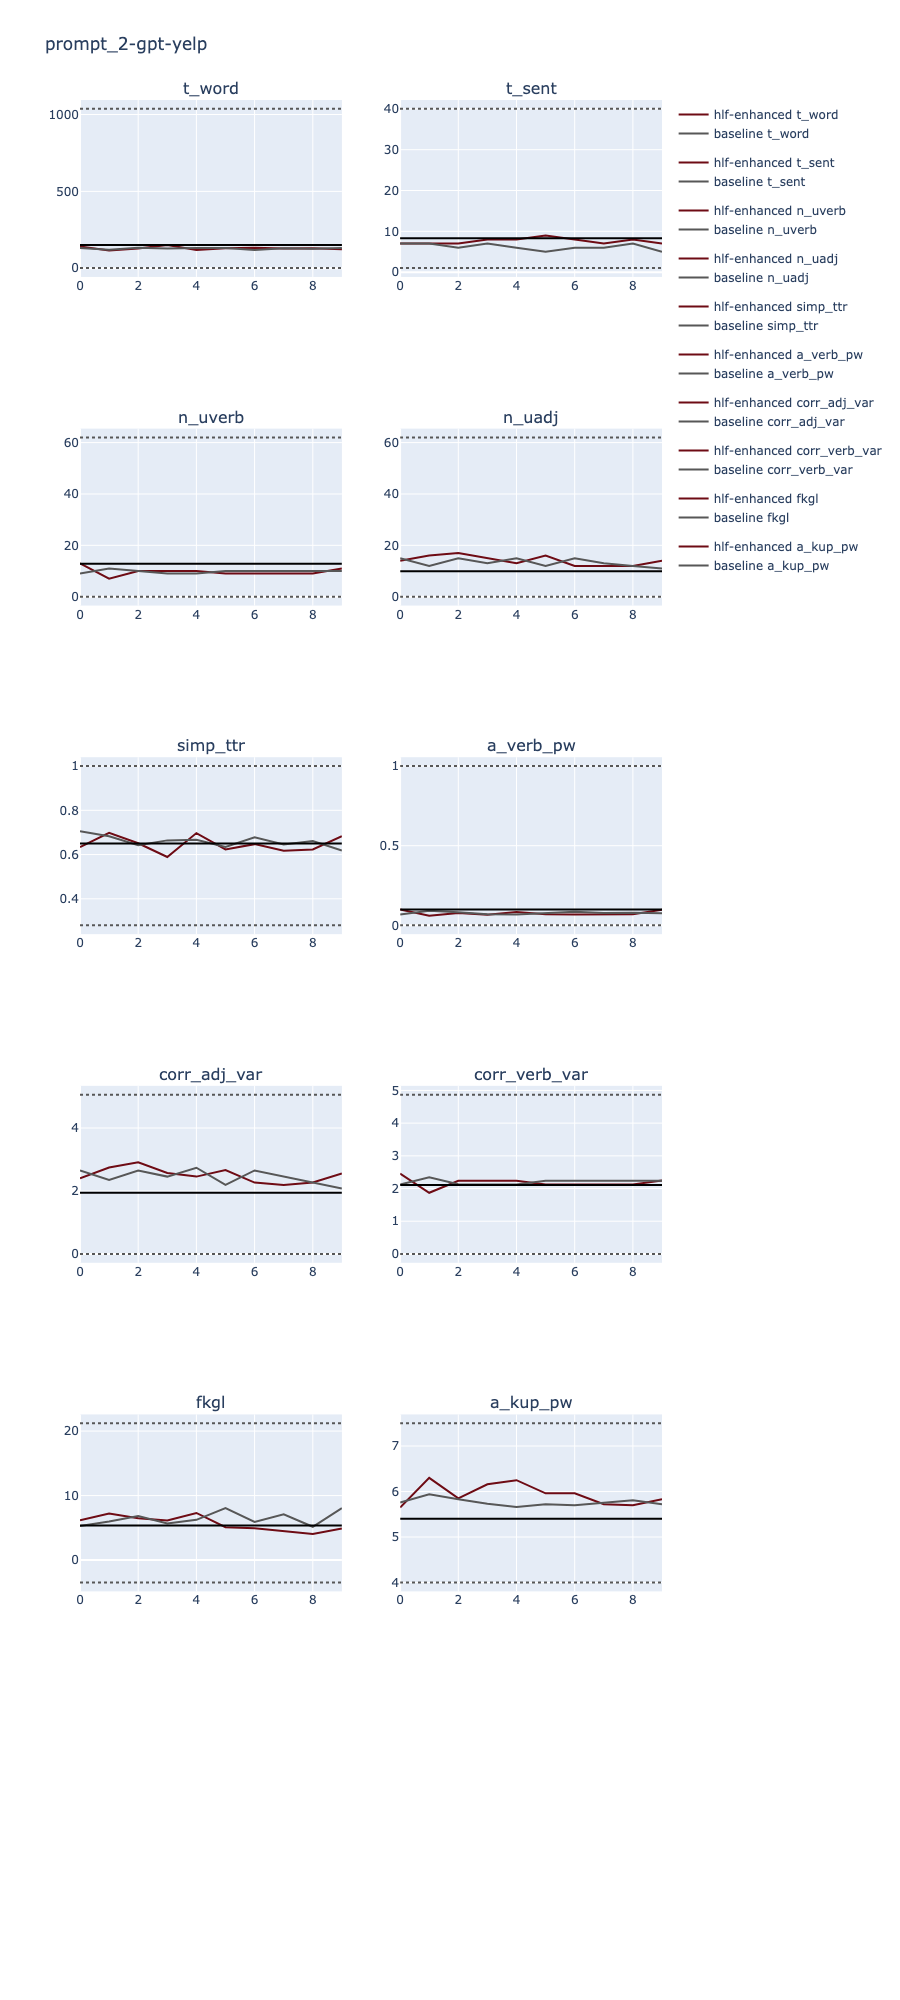
\includegraphics[width=\textwidth,height=0.9\textheight,scale=1]{plots/prompt_2_ifd/prompt_2-gpt-yelp/prompt_2-gpt-yelp.png}
    \caption{GPT on Yelp Corpus\\Prompt With Examples\\Input from Corpus}\label{fig:gpt-prompt2-yelp-ifd}
\end{figure*}

\Cref{fig:gpt-prompt1-cnn,fig:gpt-prompt1-yelp,fig:gpt-prompt2-cnn,fig:gpt-prompt2-yelp,fig:gpt-prompt2-cnn-ifd,fig:gpt-prompt2-yelp-ifd}
show the experiment results for the Claude 3 Opus large language model.

\subsection{Gemini}

\begin{figure*}[ht]
    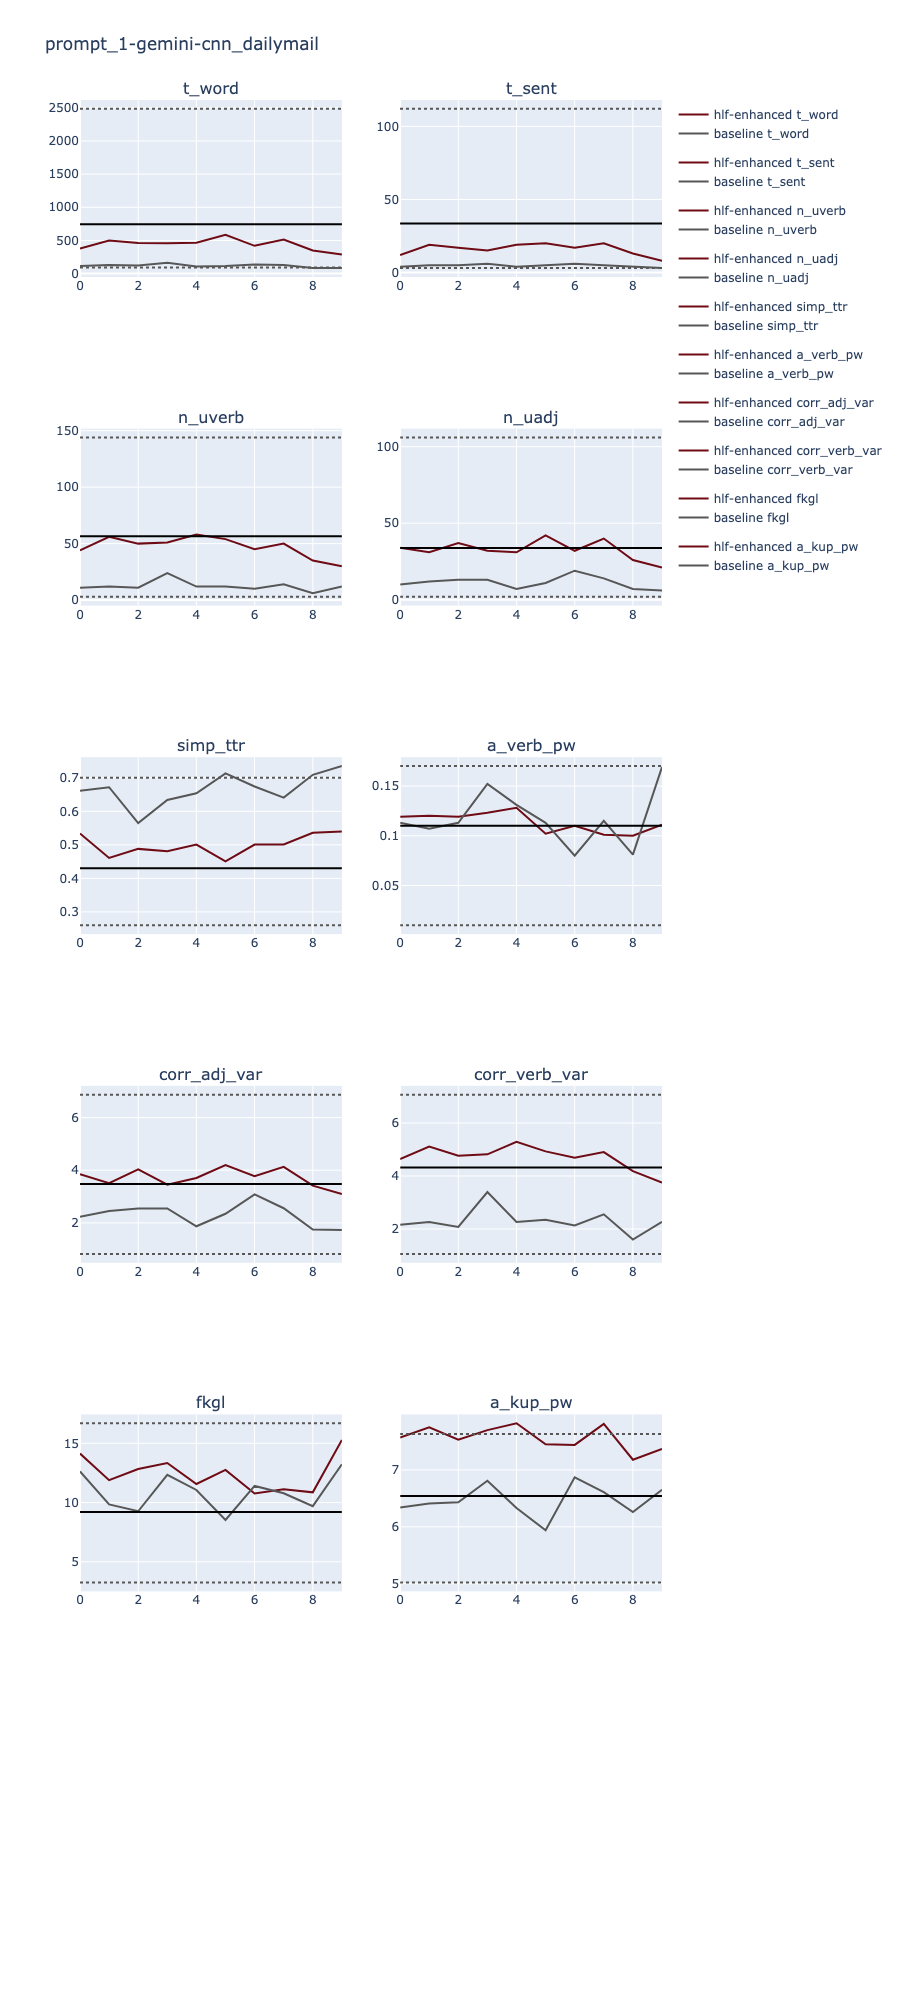
\includegraphics[width=\textwidth,height=0.9\textheight,scale=1]{plots/prompt_1/prompt_1-gemini-cnn_dailymail/prompt_1-gemini-cnn_dailymail.png}
    \caption{Gemini on CNN Corpus\\Prompt Without Examples}\label{fig:gemini-prompt1-cnn}
\end{figure*}
\begin{figure*}[ht]
    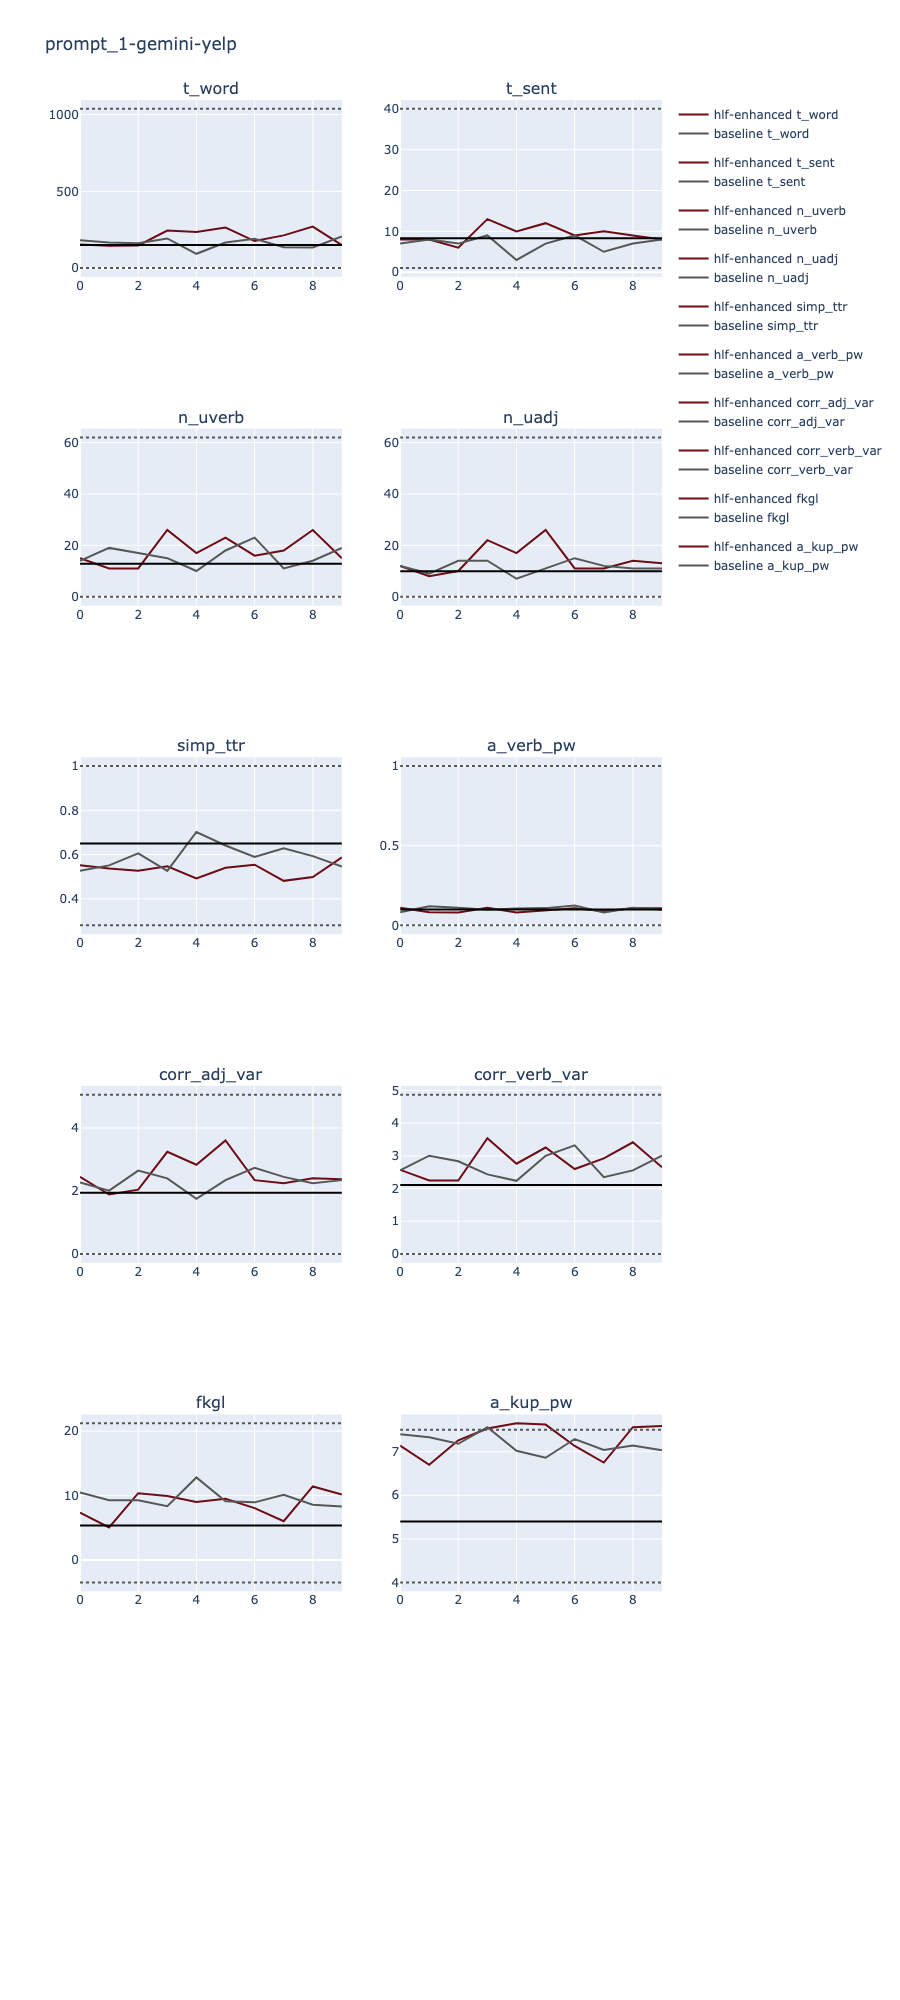
\includegraphics[width=\textwidth,height=0.9\textheight,scale=1]{plots/prompt_1/prompt_1-gemini-yelp/prompt_1-gemini-yelp.png}
    \caption{Gemini on Yelp Corpus\\Prompt Without Examples}\label{fig:gemini-prompt1-yelp}
\end{figure*}
\begin{figure*}[ht]
    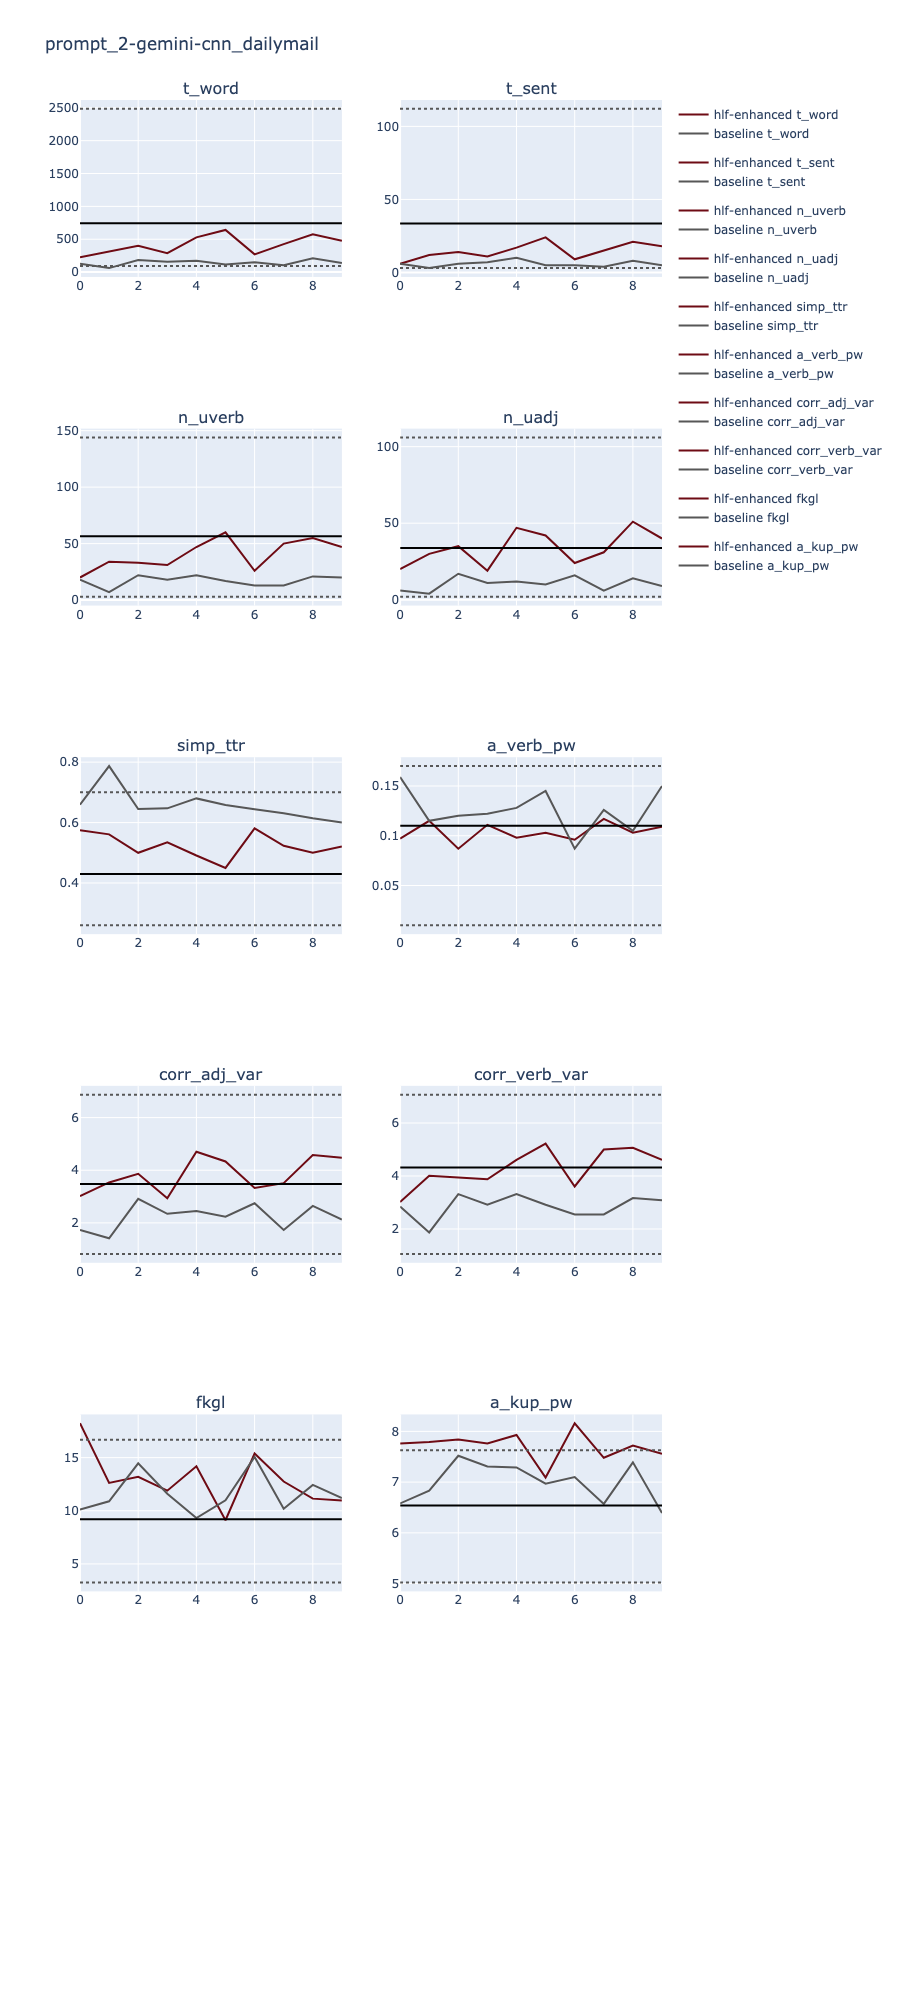
\includegraphics[width=\textwidth,height=0.9\textheight,scale=1]{plots/prompt_2/prompt_2-gemini-cnn_dailymail/prompt_2-gemini-cnn_dailymail.png}
    \caption{Gemini on CNN Corpus\\Prompt With Examples\\Extraneous Input}\label{fig:gemini-prompt2-cnn}
\end{figure*}
\begin{figure*}[ht]
    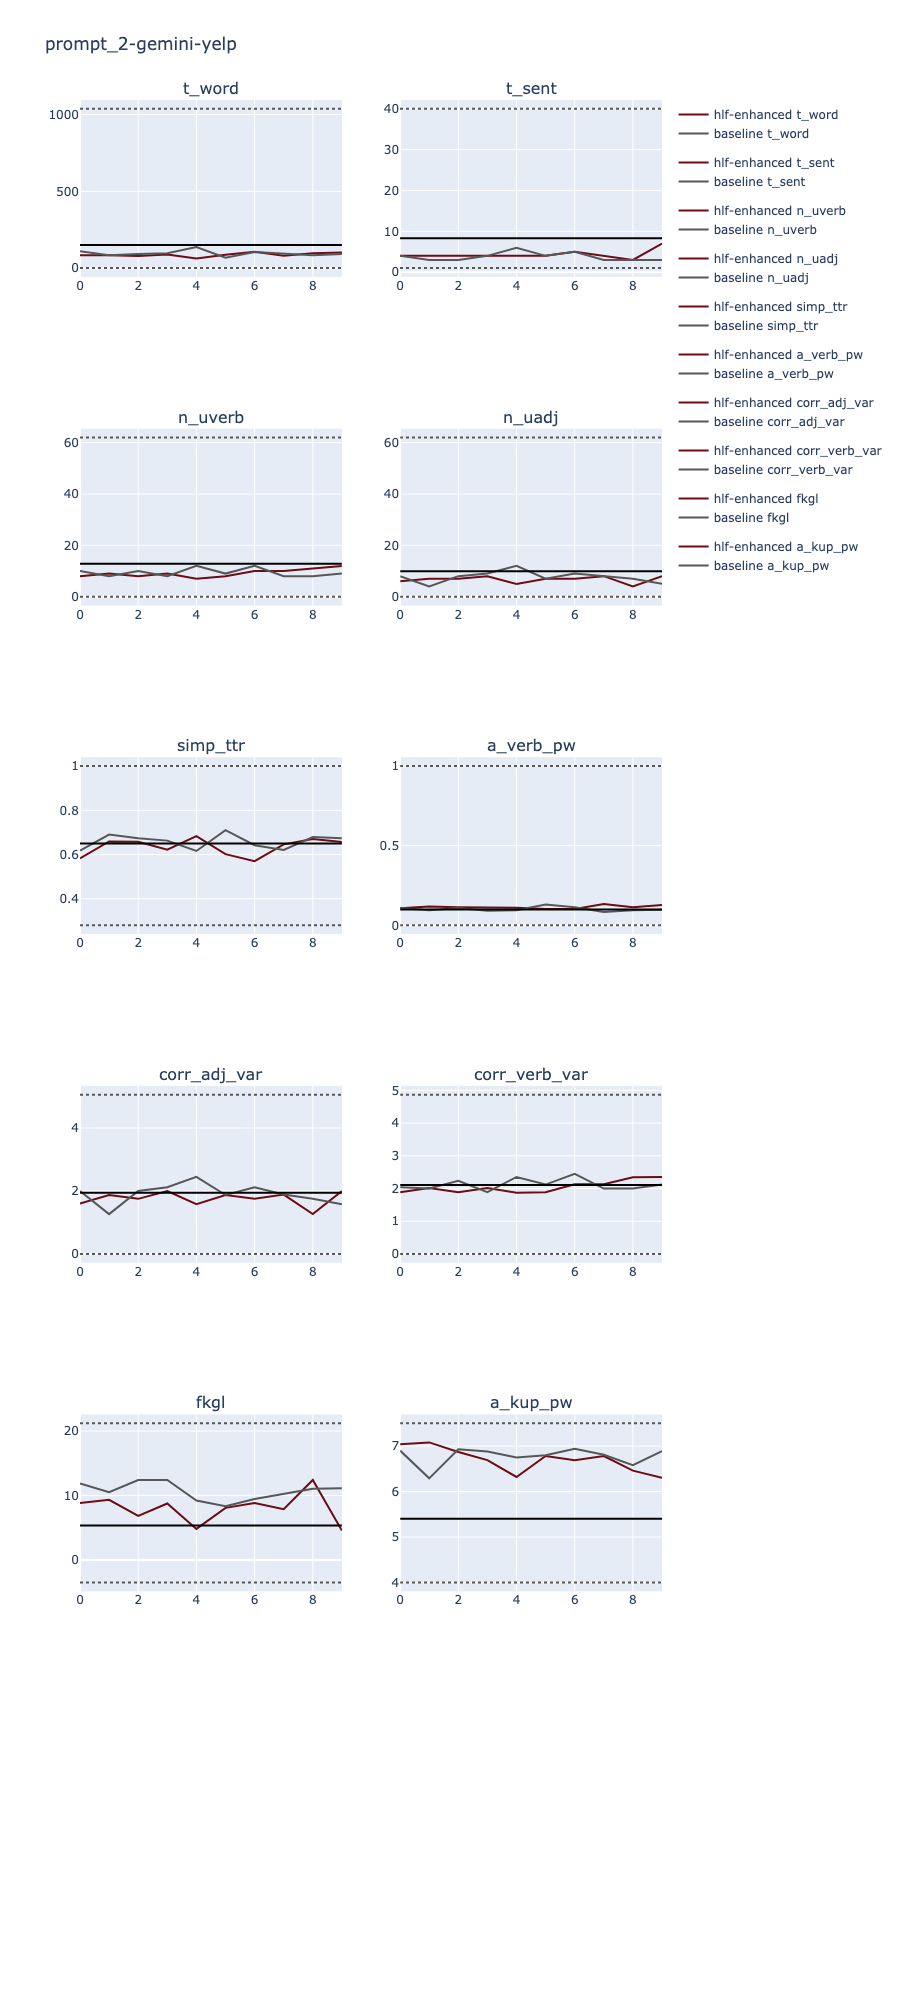
\includegraphics[width=\textwidth,height=0.9\textheight,scale=1]{plots/prompt_2/prompt_2-gemini-yelp/prompt_2-gemini-yelp.png}
    \caption{Gemini on Yelp Corpus\\Prompt With Examples\\Extraneous Input}\label{fig:gemini-prompt2-yelp}
\end{figure*}
\begin{figure*}[ht]
    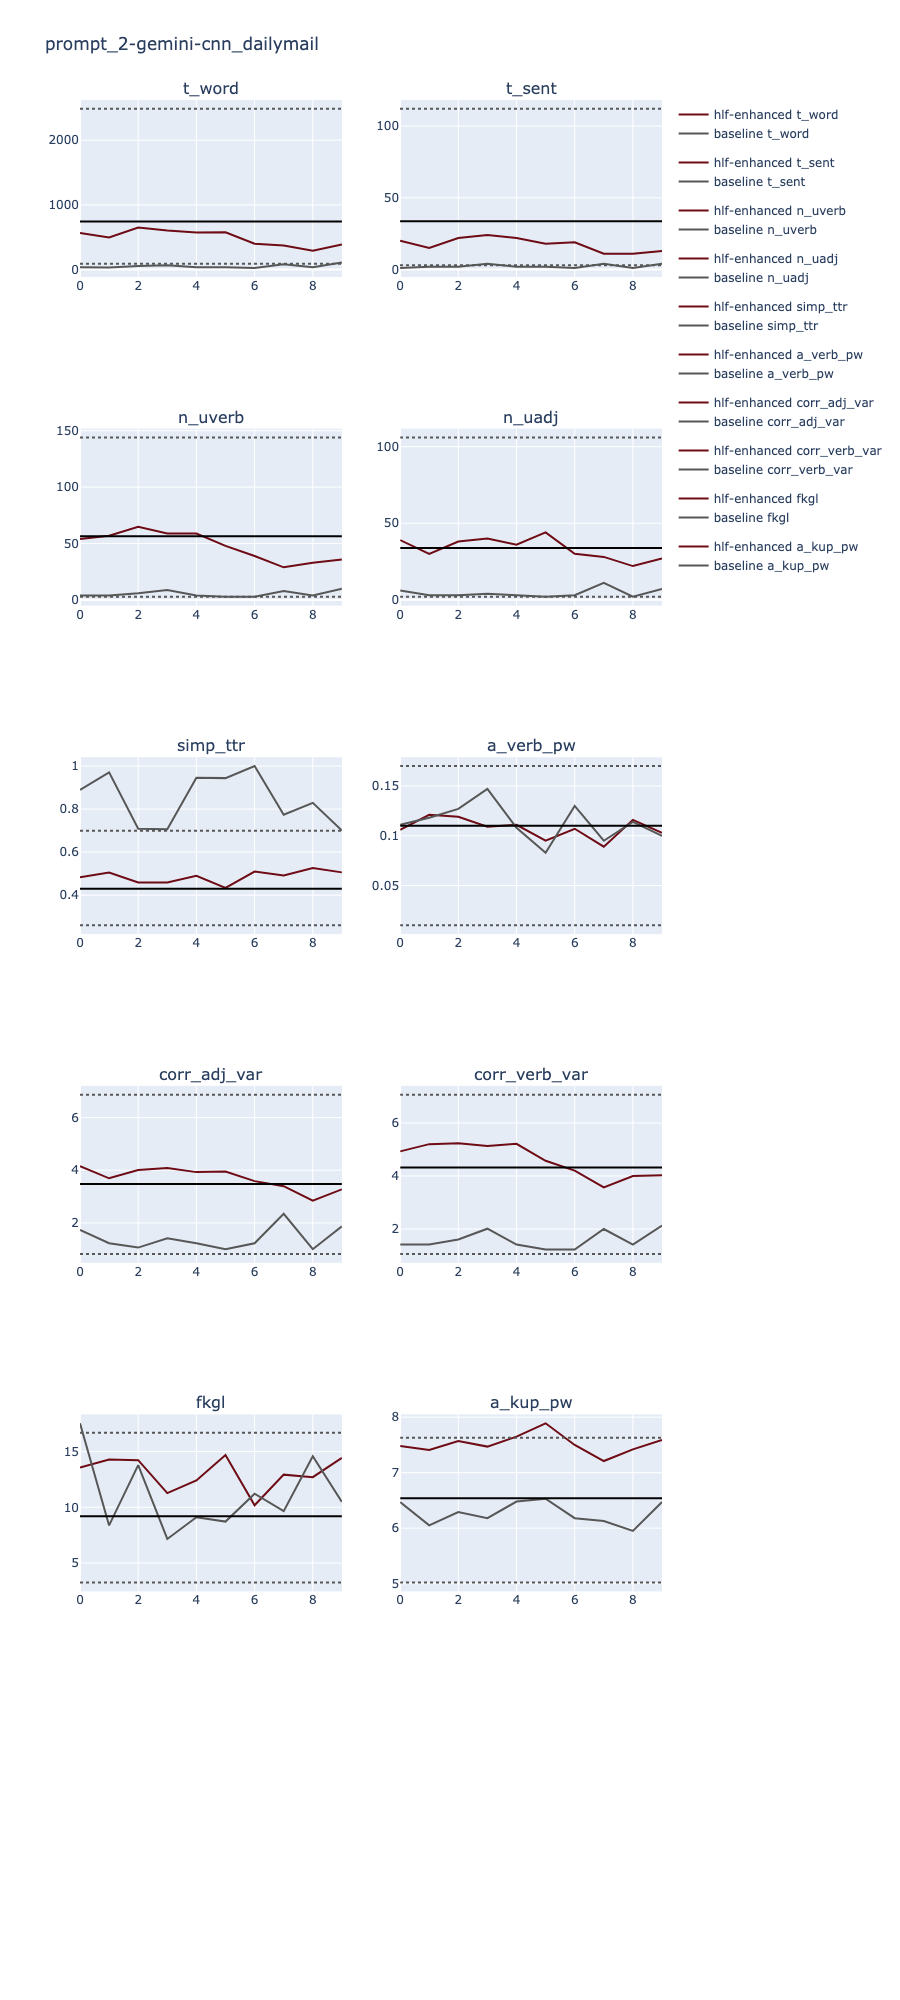
\includegraphics[width=\textwidth,height=0.9\textheight,scale=1]{plots/prompt_2_ifd/prompt_2-gemini-cnn_dailymail/prompt_2-gemini-cnn_dailymail.png}
    \caption{Gemini on CNN Corpus\\Prompt With Examples\\Input from Corpus}\label{fig:gemini-prompt2-cnn-ifd}
\end{figure*}
\begin{figure*}[ht]
    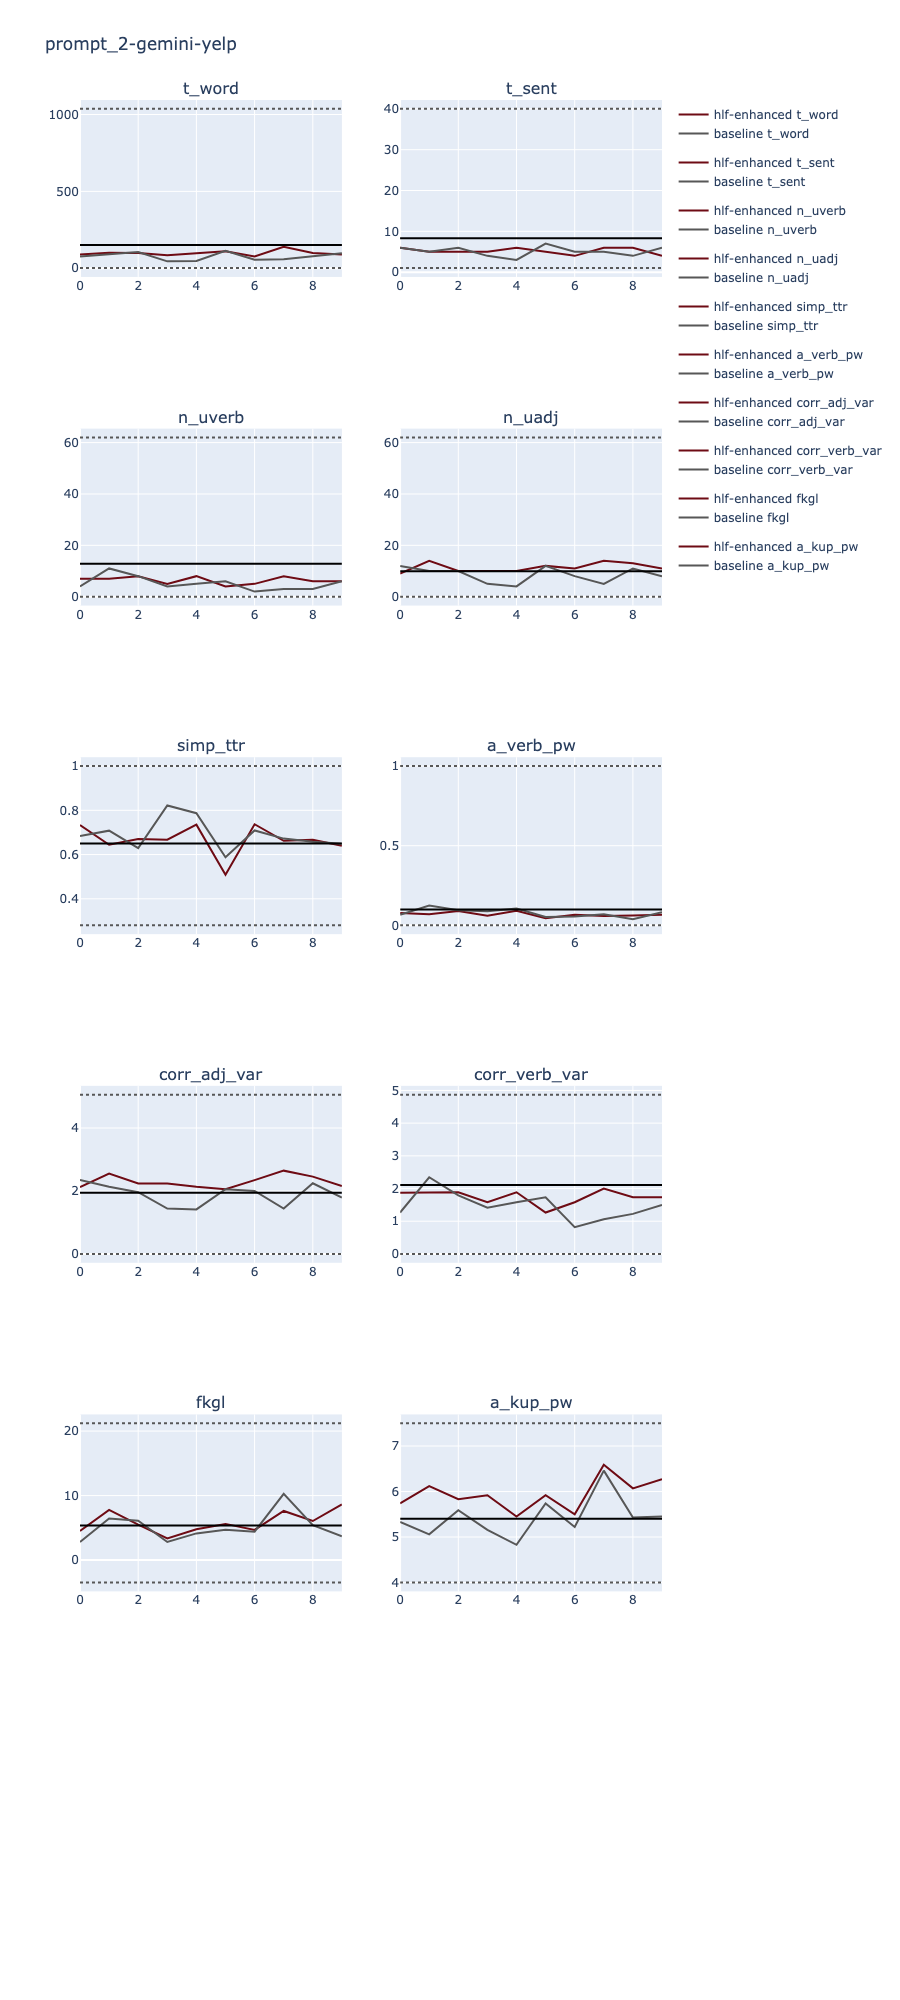
\includegraphics[width=\textwidth,height=0.9\textheight,scale=1]{plots/prompt_2_ifd/prompt_2-gemini-yelp/prompt_2-gemini-yelp.png}
    \caption{Gemini on Yelp Corpus\\Prompt With Examples\\Input from Corpus}\label{fig:gemini-prompt2-yelp-ifd}
\end{figure*}

\Cref{fig:gemini-prompt1-cnn,fig:gemini-prompt1-yelp,fig:gemini-prompt2-cnn,fig:gemini-prompt2-yelp,fig:gemini-prompt2-cnn-ifd,fig:gemini-prompt2-yelp-ifd}
show the experiment results for the Claude 3 Opus large language model.

\subsection{Claude3}

\begin{figure*}[ht]
    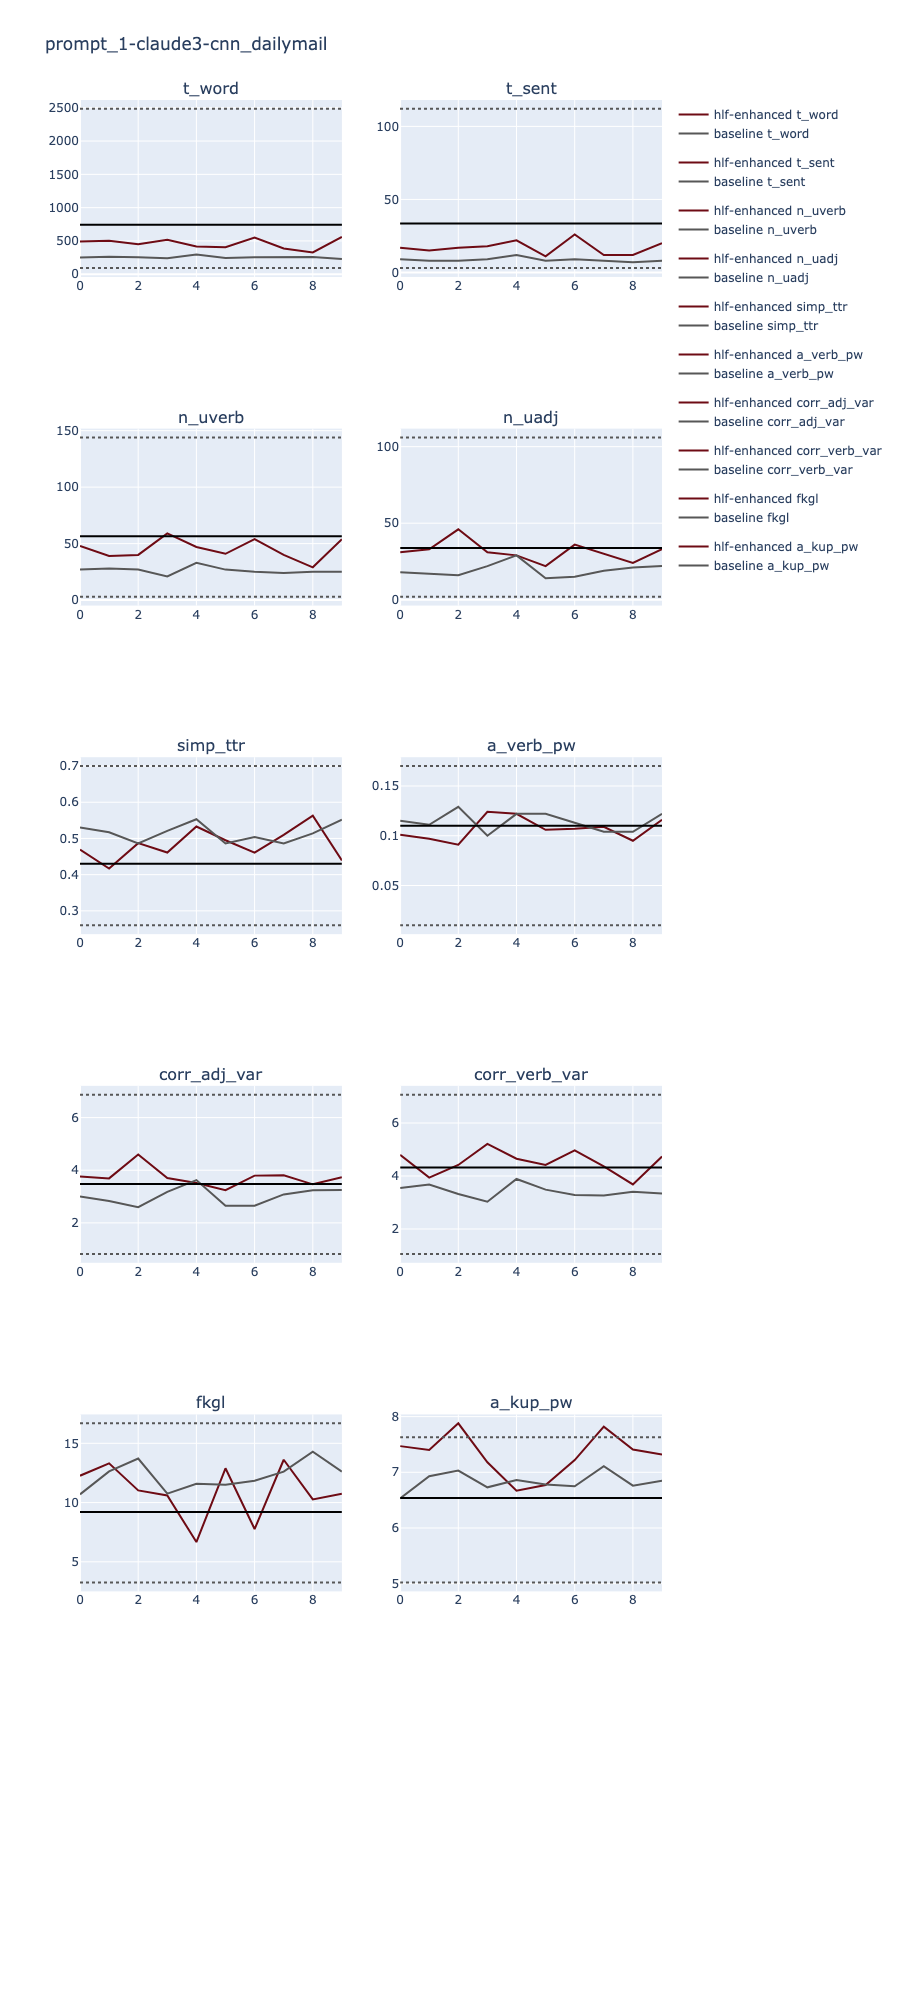
\includegraphics[width=\textwidth,height=0.9\textheight,scale=1]{plots/prompt_1/prompt_1-claude3-cnn_dailymail/prompt_1-claude3-cnn_dailymail.png}
    \caption{Claude3 on CNN Corpus\\Prompt Without Examples}\label{fig:claude3-prompt1-cnn}
\end{figure*}
\begin{figure*}[ht]
    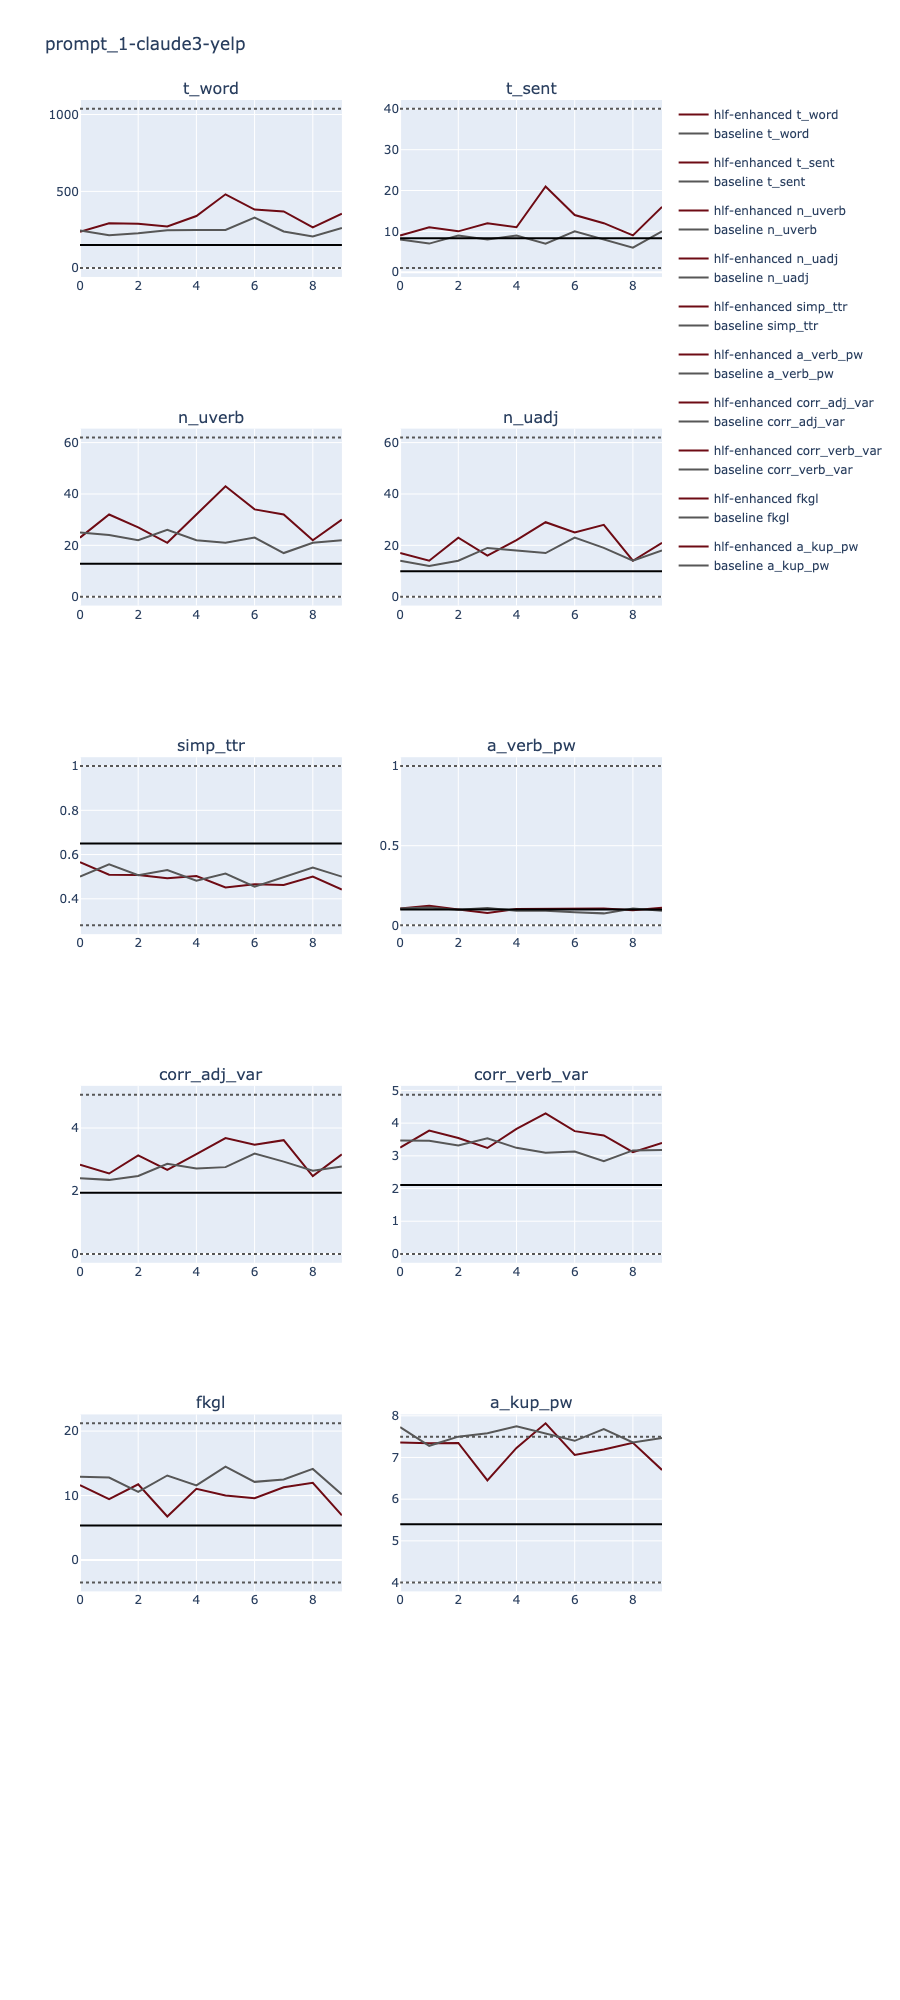
\includegraphics[width=\textwidth,height=0.9\textheight,scale=1]{plots/prompt_1/prompt_1-claude3-yelp/prompt_1-claude3-yelp.png}
    \caption{Claude3 on Yelp Corpus\\Prompt Without Examples}\label{fig:claude3-prompt1-yelp}
\end{figure*}
\begin{figure*}[ht]
    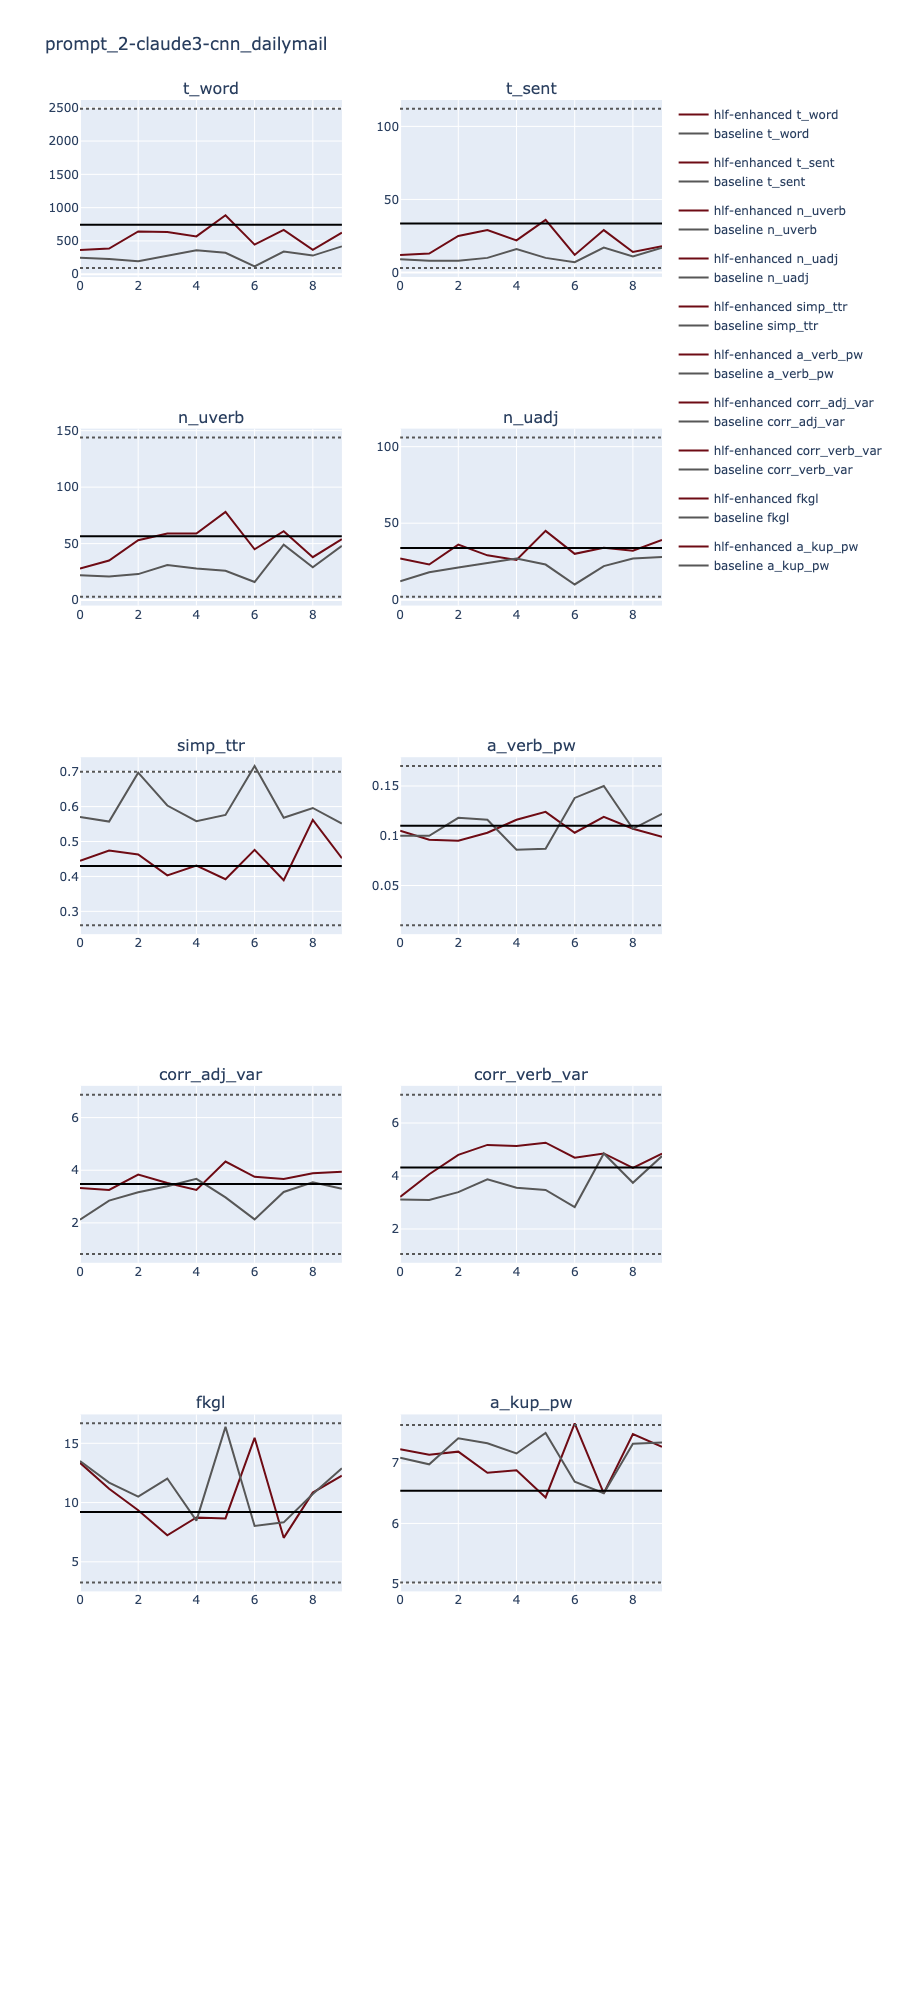
\includegraphics[width=\textwidth,height=0.9\textheight,scale=1]{plots/prompt_2/prompt_2-claude3-cnn_dailymail/prompt_2-claude3-cnn_dailymail.png}
    \caption{Claude3 on CNN Corpus\\Prompt With Examples\\Extraneous Input}\label{fig:claude3-prompt2-cnn}
\end{figure*}
\begin{figure*}[ht]
    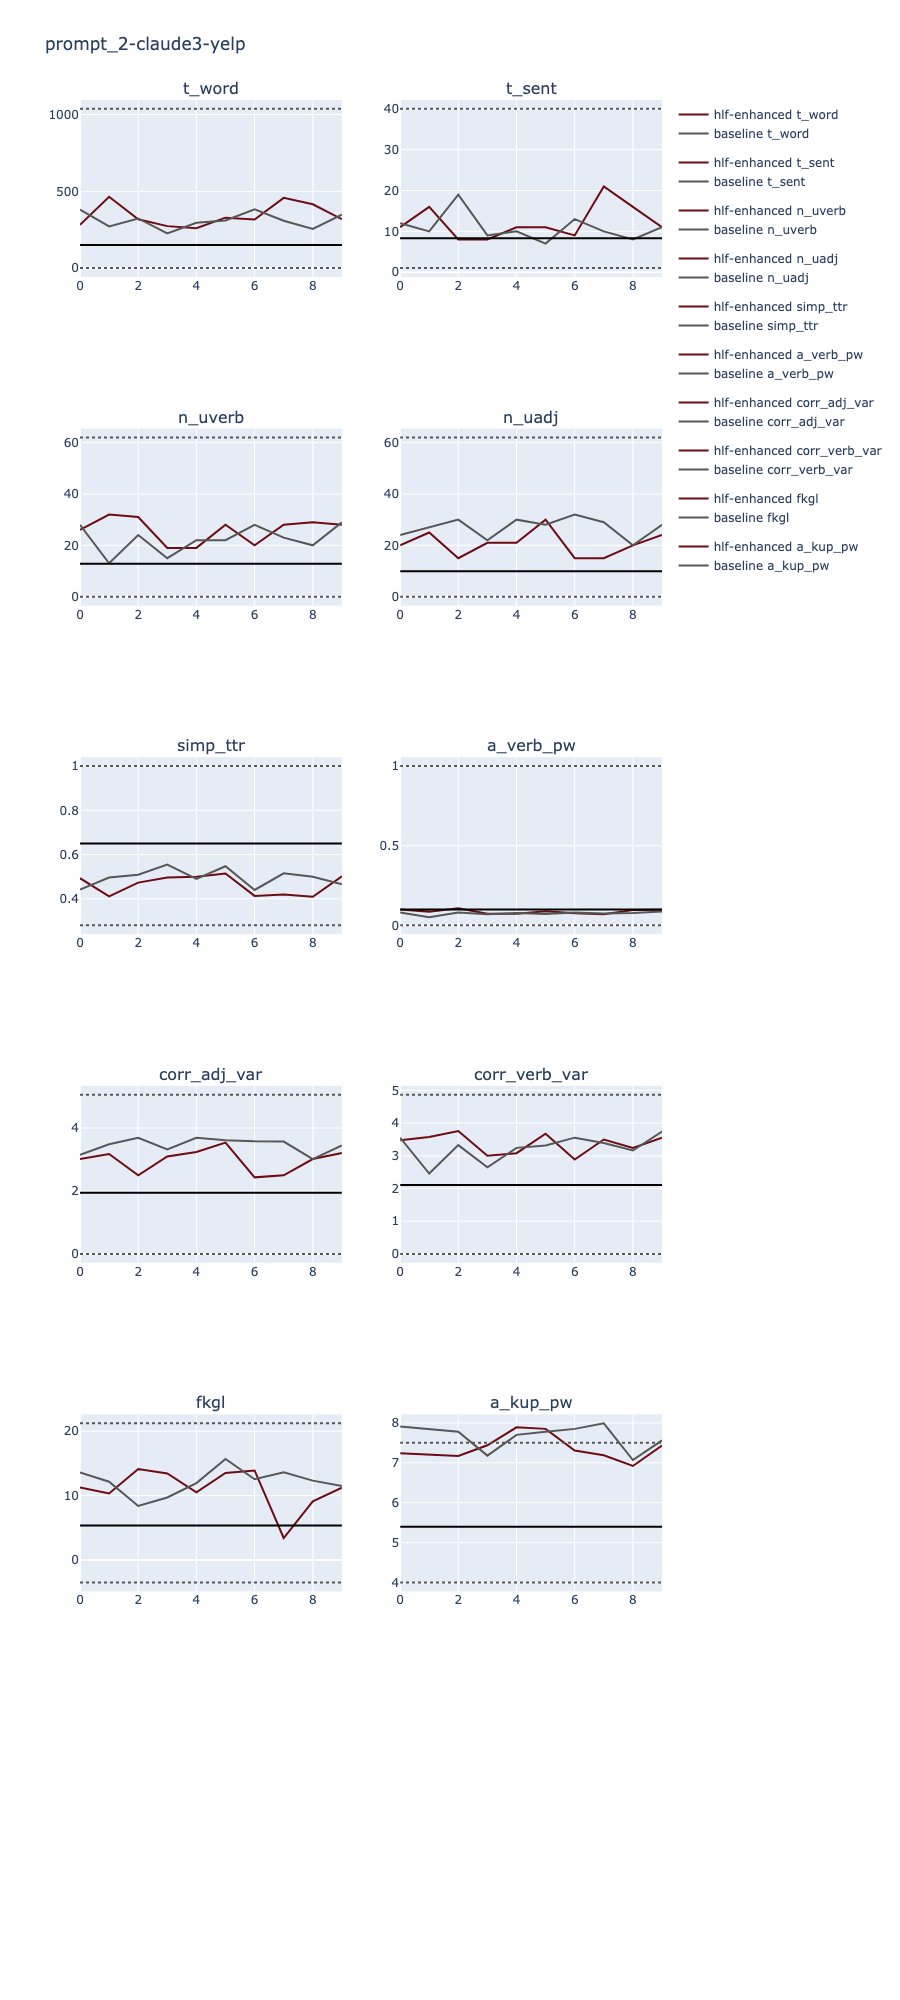
\includegraphics[width=\textwidth,height=0.9\textheight,scale=1]{plots/prompt_2/prompt_2-claude3-yelp/prompt_2-claude3-yelp.png}
    \caption{Claude3 on Yelp Corpus\\Prompt With Examples\\Extraneous Input}\label{fig:claude3-prompt2-yelp}
\end{figure*}
\begin{figure*}[ht]
    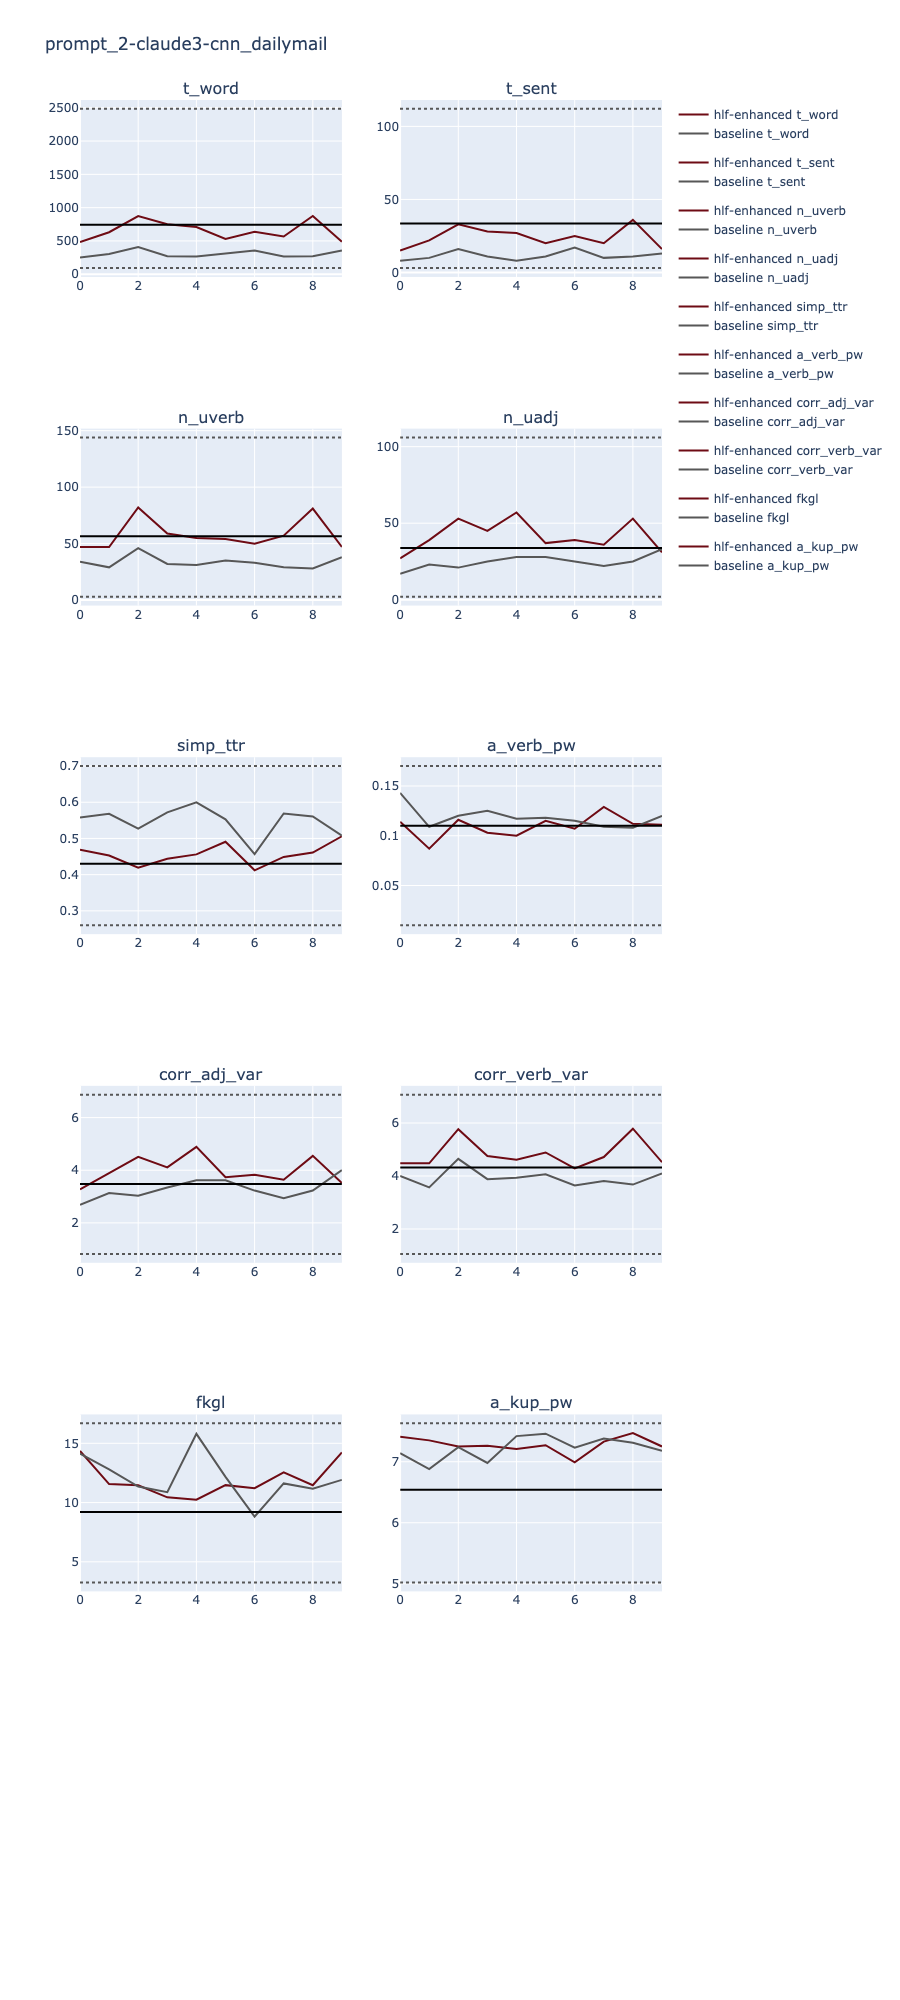
\includegraphics[width=\textwidth,height=0.9\textheight,scale=1]{plots/prompt_2_ifd/prompt_2-claude3-cnn_dailymail/prompt_2-claude3-cnn_dailymail.png}
    \caption{Claude3 on CNN Corpus\\Prompt With Examples\\Input from Corpus}\label{fig:claude3-prompt2-cnn-ifd}
\end{figure*}
\begin{figure*}[ht]
    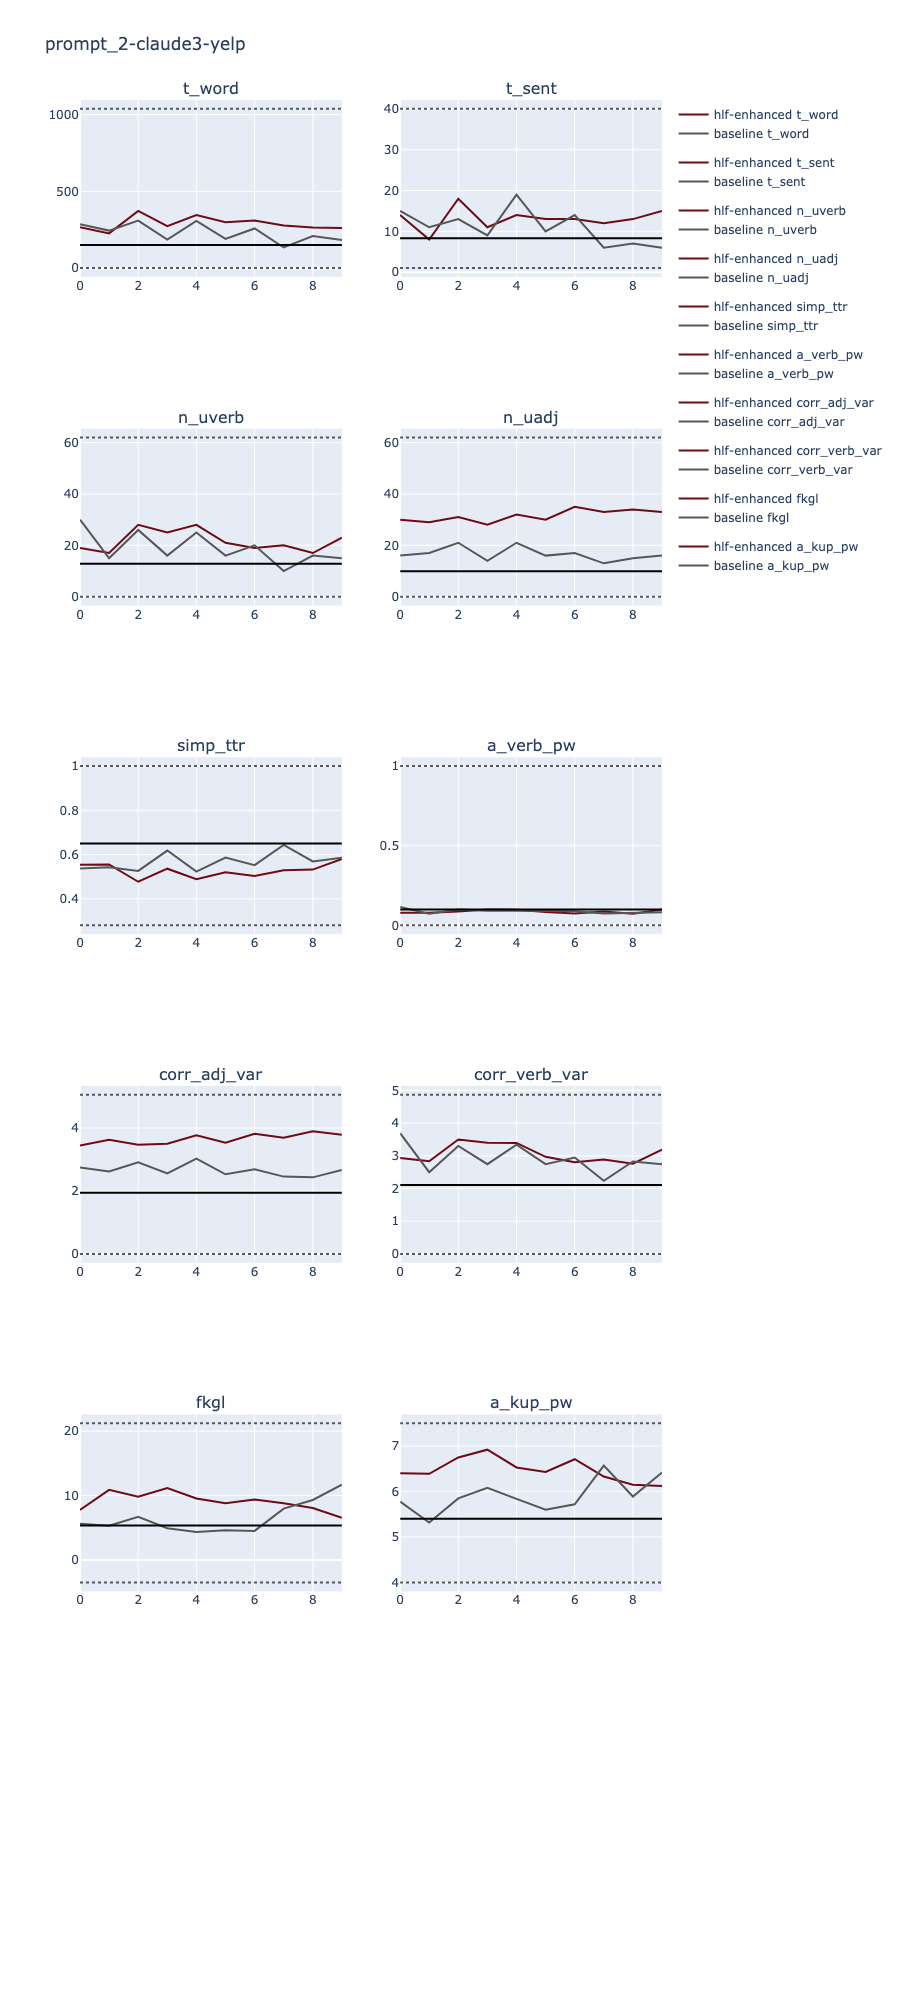
\includegraphics[width=\textwidth,height=0.9\textheight,scale=1]{plots/prompt_2_ifd/prompt_2-claude3-yelp/prompt_2-claude3-yelp.png}
    \caption{Claude3 on Yelp Corpus\\Prompt With Examples\\Input from Corpus}\label{fig:claude3-prompt2-yelp-ifd}
\end{figure*}

\Cref{fig:claude3-prompt1-cnn,fig:claude3-prompt1-yelp,fig:claude3-prompt2-cnn,fig:claude3-prompt2-yelp,fig:claude3-prompt2-cnn-ifd,fig:claude3-prompt2-yelp-ifd}
show the experiment results for the Claude 3 Opus large language model.

\subsection{Llama3}

\begin{figure*}[ht]
    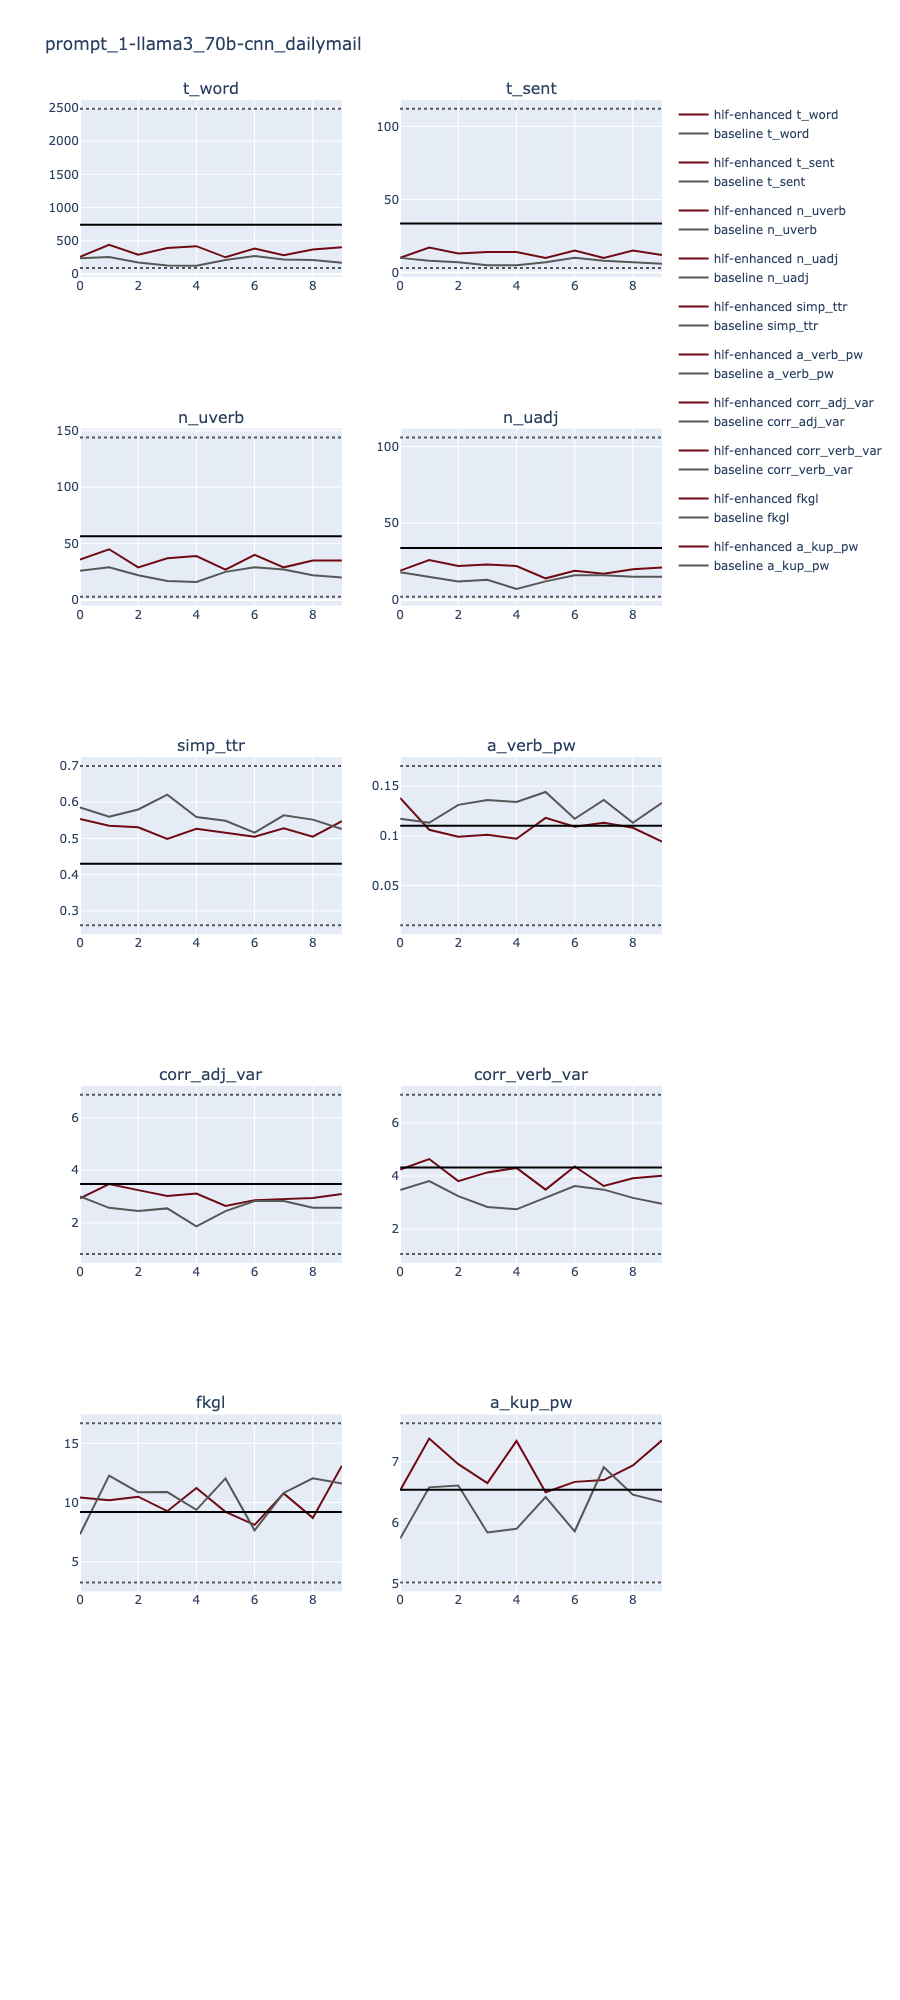
\includegraphics[width=\textwidth,height=0.9\textheight,scale=1]{plots/prompt_1/prompt_1-llama3_70b-cnn_dailymail/prompt_1-llama3_70b-cnn_dailymail.png}
    \caption{Llama3 on CNN Corpus\\Prompt Without Examples}\label{fig:llama3_70b-prompt1-cnn}
\end{figure*}
\begin{figure*}[ht]
    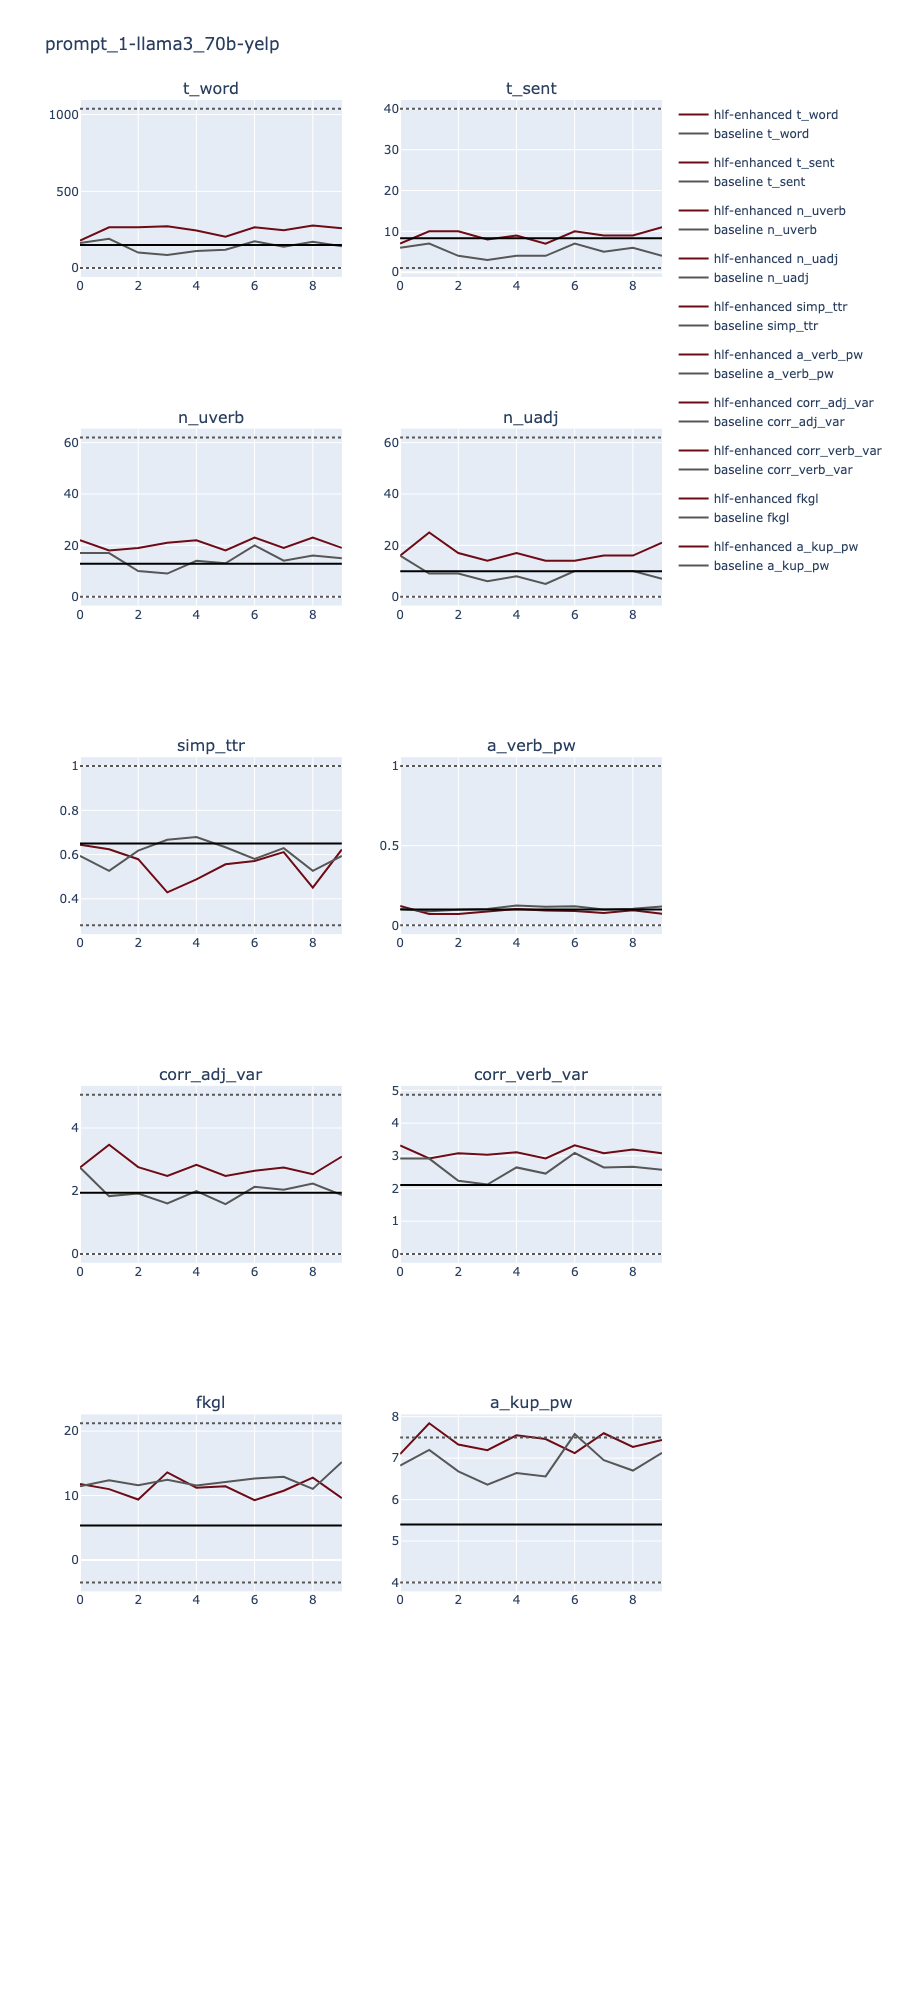
\includegraphics[width=\textwidth,height=0.9\textheight,scale=1]{plots/prompt_1/prompt_1-llama3_70b-yelp/prompt_1-llama3_70b-yelp.png}
    \caption{Llama3 on Yelp Corpus\\Prompt Without Examples}\label{fig:llama3_70b-prompt1-yelp}
\end{figure*}
\begin{figure*}[ht]
    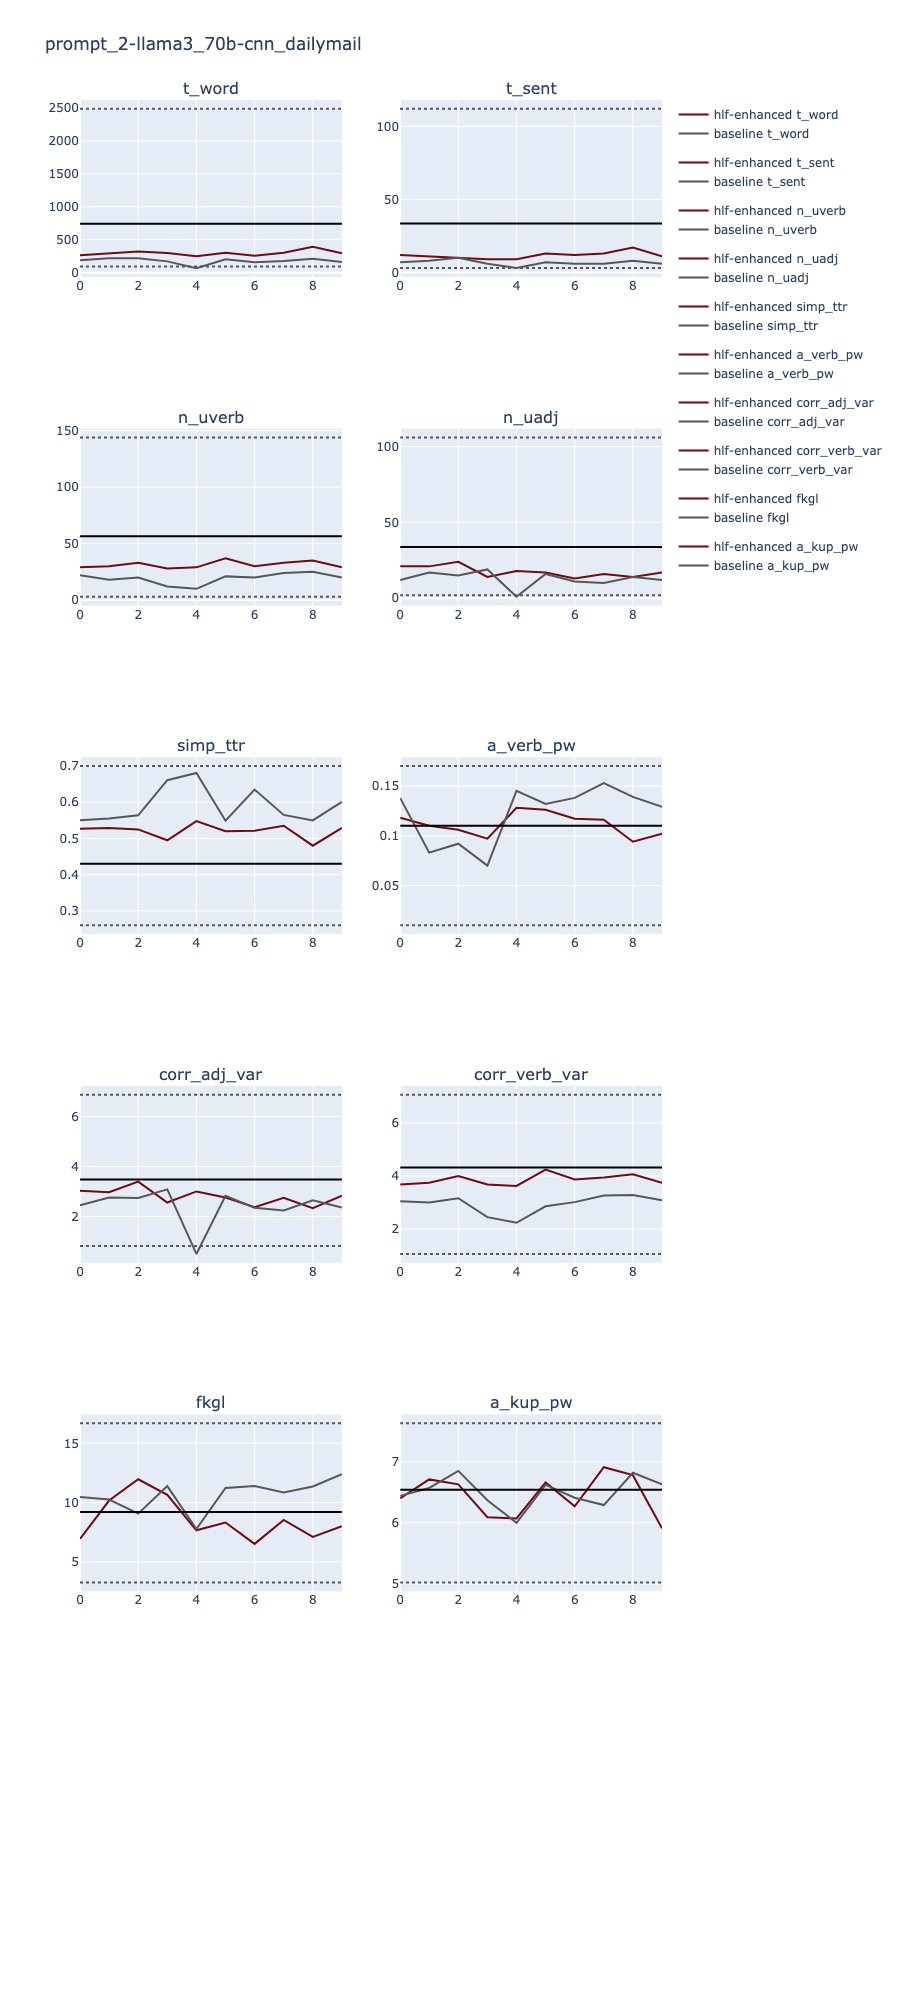
\includegraphics[width=\textwidth,height=0.9\textheight,scale=1]{plots/prompt_2/prompt_2-llama3_70b-cnn_dailymail/prompt_2-llama3_70b-cnn_dailymail.png}
    \caption{Llama3 on CNN Corpus\\Prompt With Examples\\Extraneous Input}\label{fig:llama3_70b-prompt2-cnn}
\end{figure*}
\begin{figure*}[ht]
    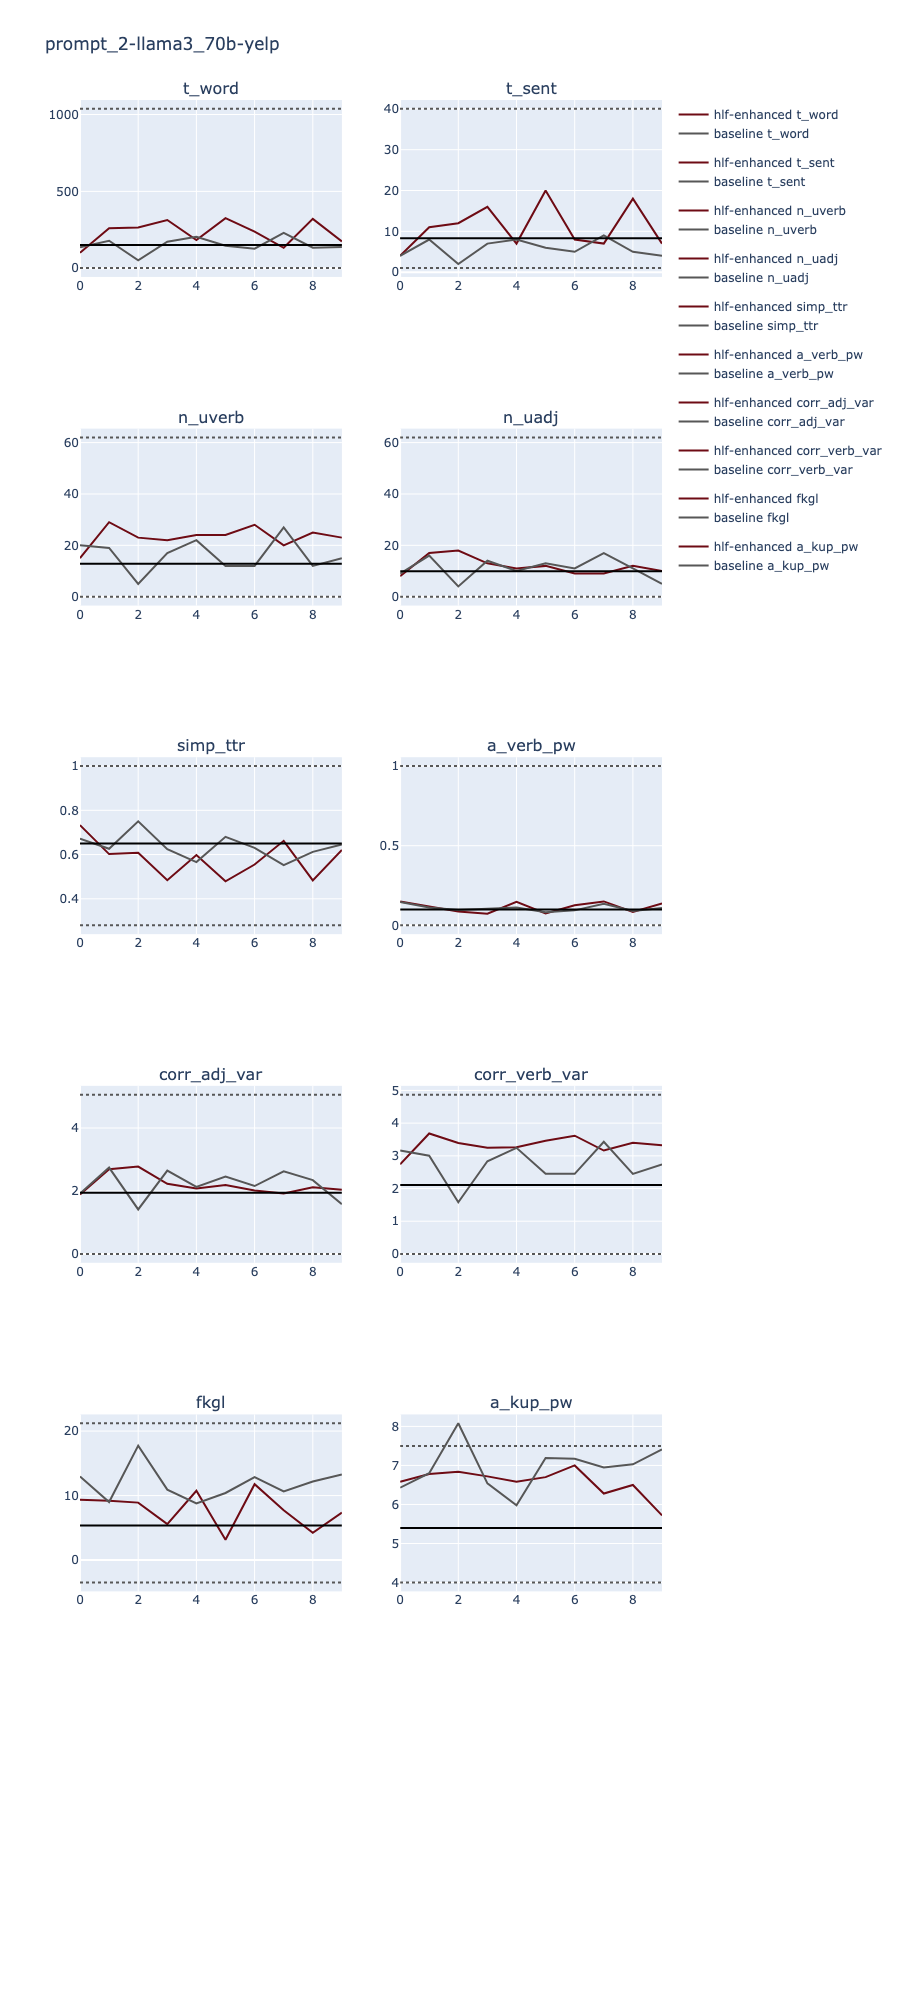
\includegraphics[width=\textwidth,height=0.9\textheight,scale=1]{plots/prompt_2/prompt_2-llama3_70b-yelp/prompt_2-llama3_70b-yelp.png}
    \caption{Llama3 on Yelp Corpus\\Prompt With Examples\\Extraneous Input}\label{fig:llama3_70b-prompt2-yelp}
\end{figure*}
\begin{figure*}[ht]
    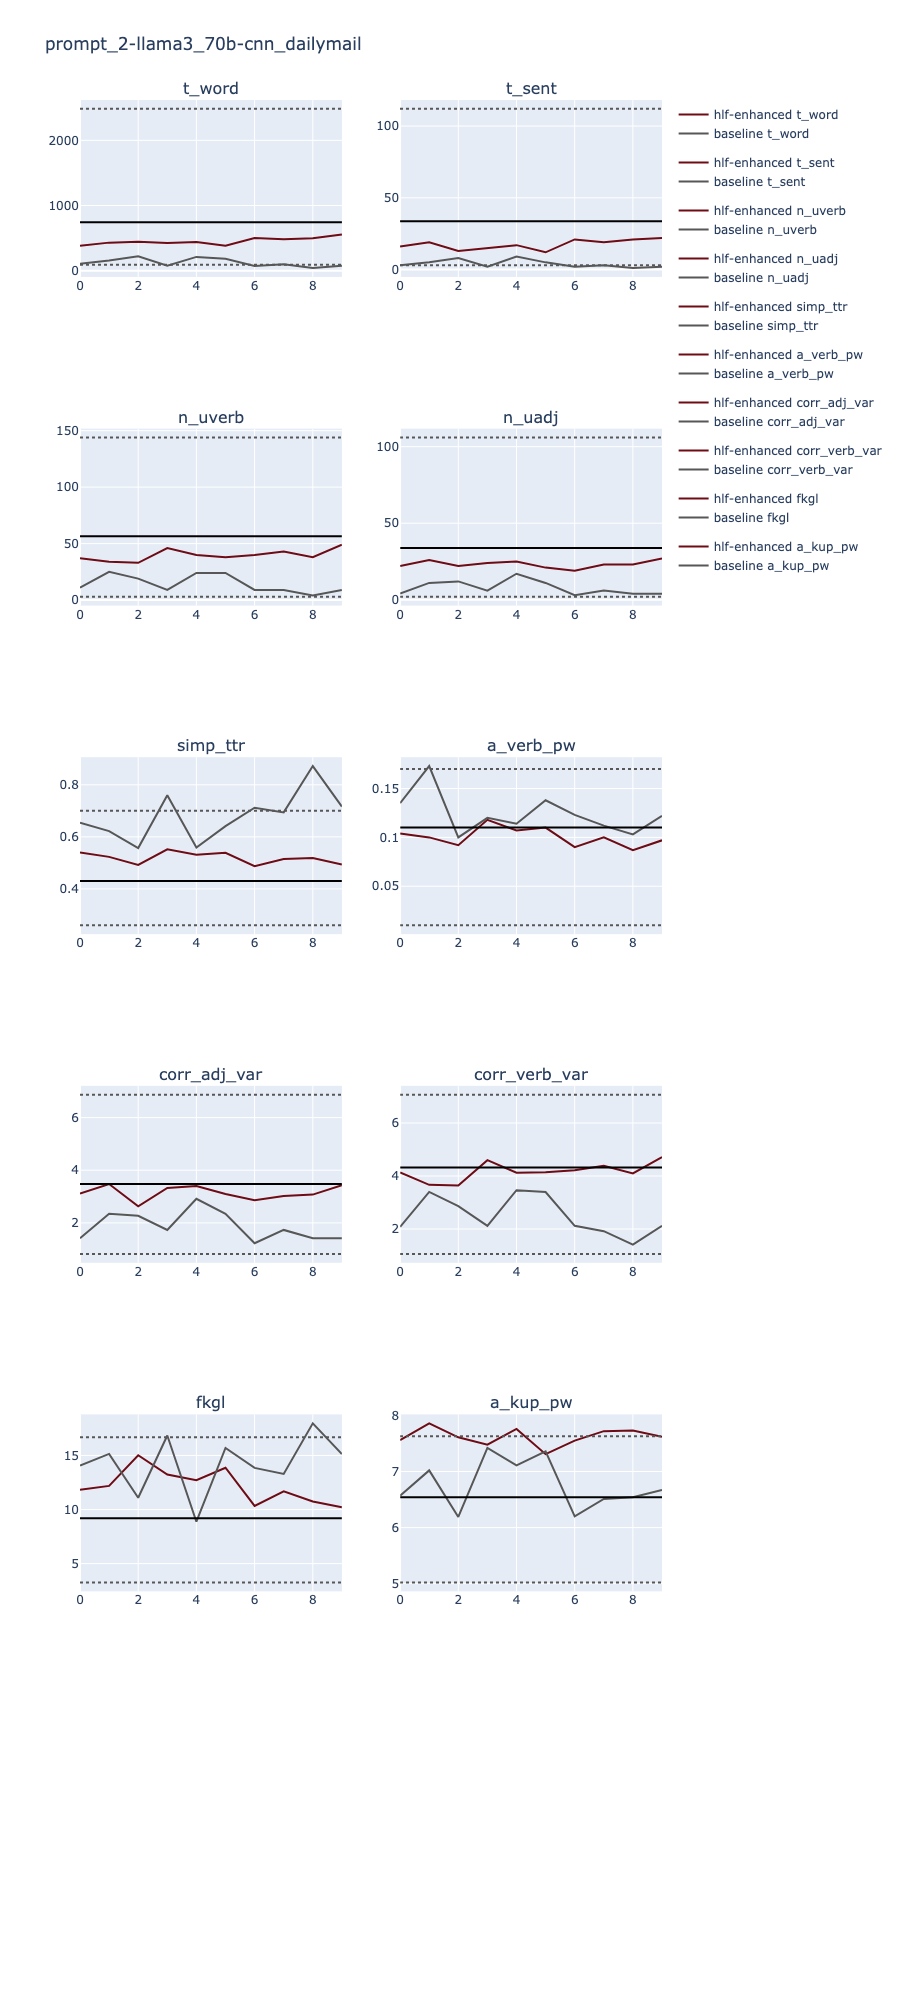
\includegraphics[width=\textwidth,height=0.9\textheight,scale=1]{plots/prompt_2_ifd/prompt_2-llama3_70b-cnn_dailymail/prompt_2-llama3_70b-cnn_dailymail.png}
    \caption{Llama3 on CNN Corpus\\Prompt With Examples\\Input from Corpus}\label{fig:llama3_70b-prompt2-cnn-ifd}
\end{figure*}
\begin{figure*}[ht]
    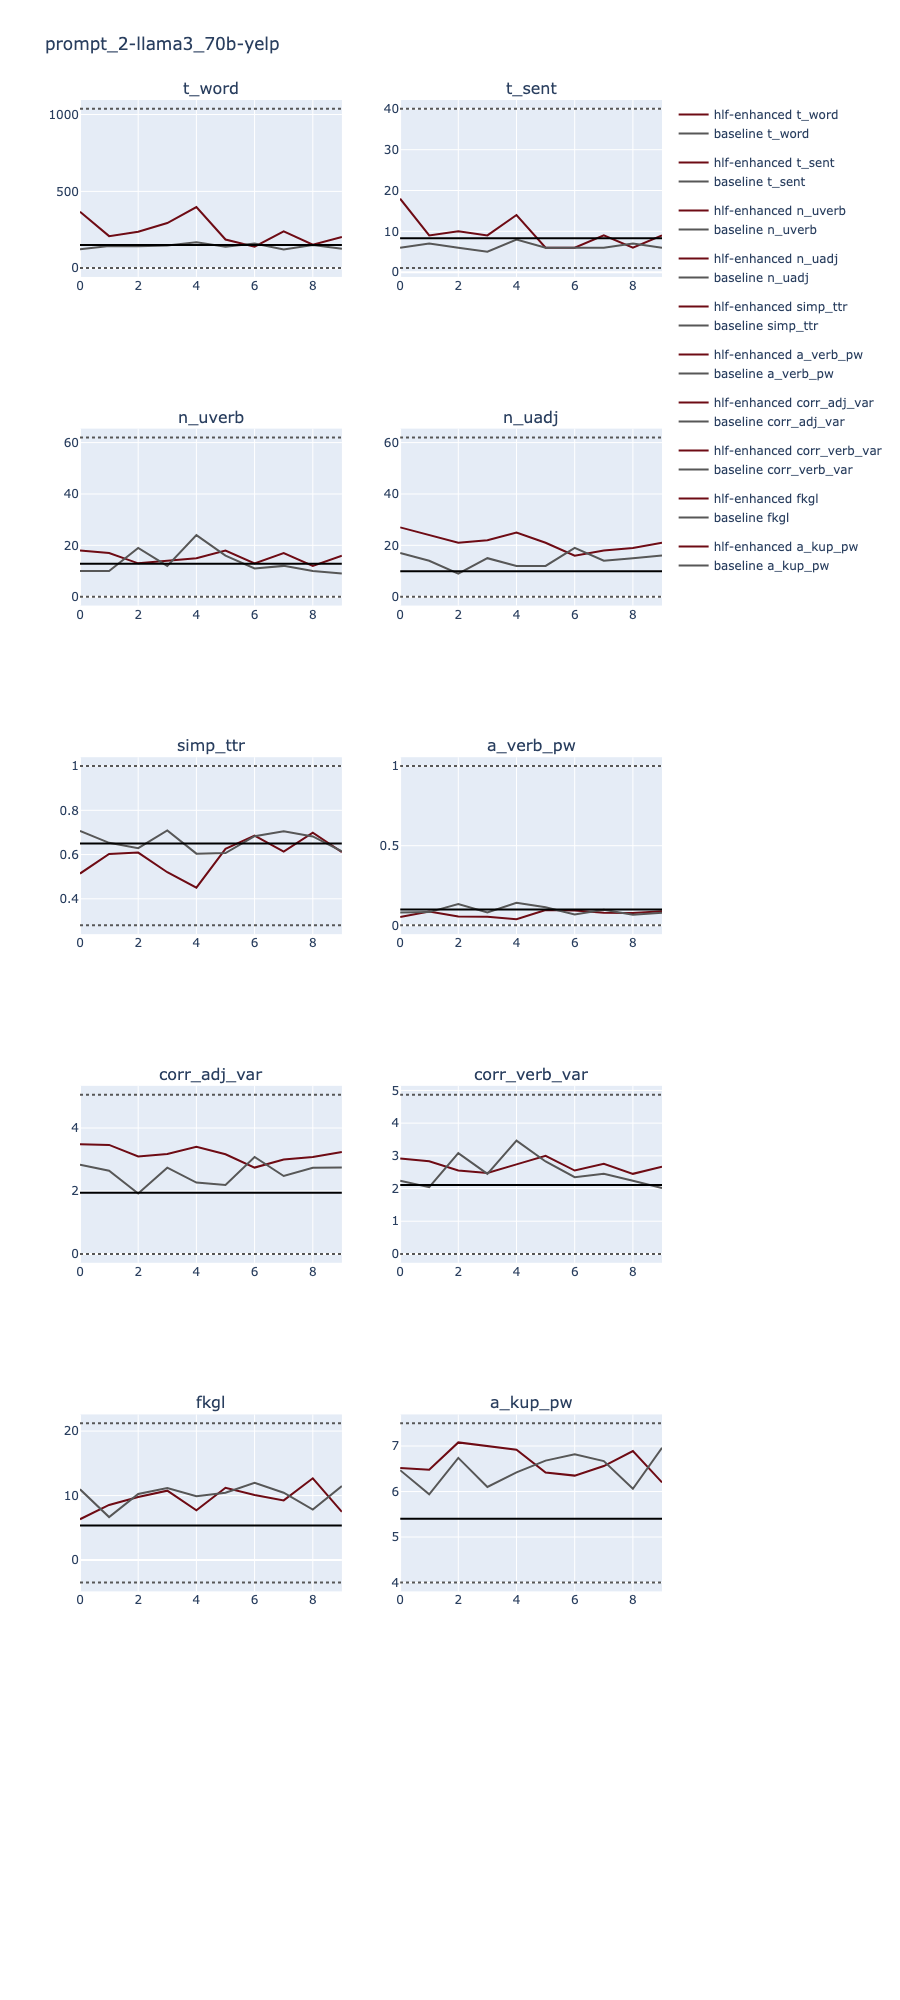
\includegraphics[width=\textwidth,height=0.9\textheight,scale=1]{plots/prompt_2_ifd/prompt_2-llama3_70b-yelp/prompt_2-llama3_70b-yelp.png}
    \caption{Llama3 on Yelp Corpus\\Prompt With Examples\\Input from Corpus}\label{fig:llama3_70b-prompt2-yelp-ifd}
\end{figure*}

\Cref{fig:llama3_70b-prompt1-cnn,fig:llama3_70b-prompt1-yelp,fig:llama3_70b-prompt2-cnn,fig:llama3_70b-prompt2-yelp,fig:llama3_70b-prompt2-cnn-ifd,fig:llama3_70b-prompt2-yelp-ifd}
show the experiment results for the Claude 3 Opus large language model.

\subsection{Command R+}

\begin{figure*}[ht]
    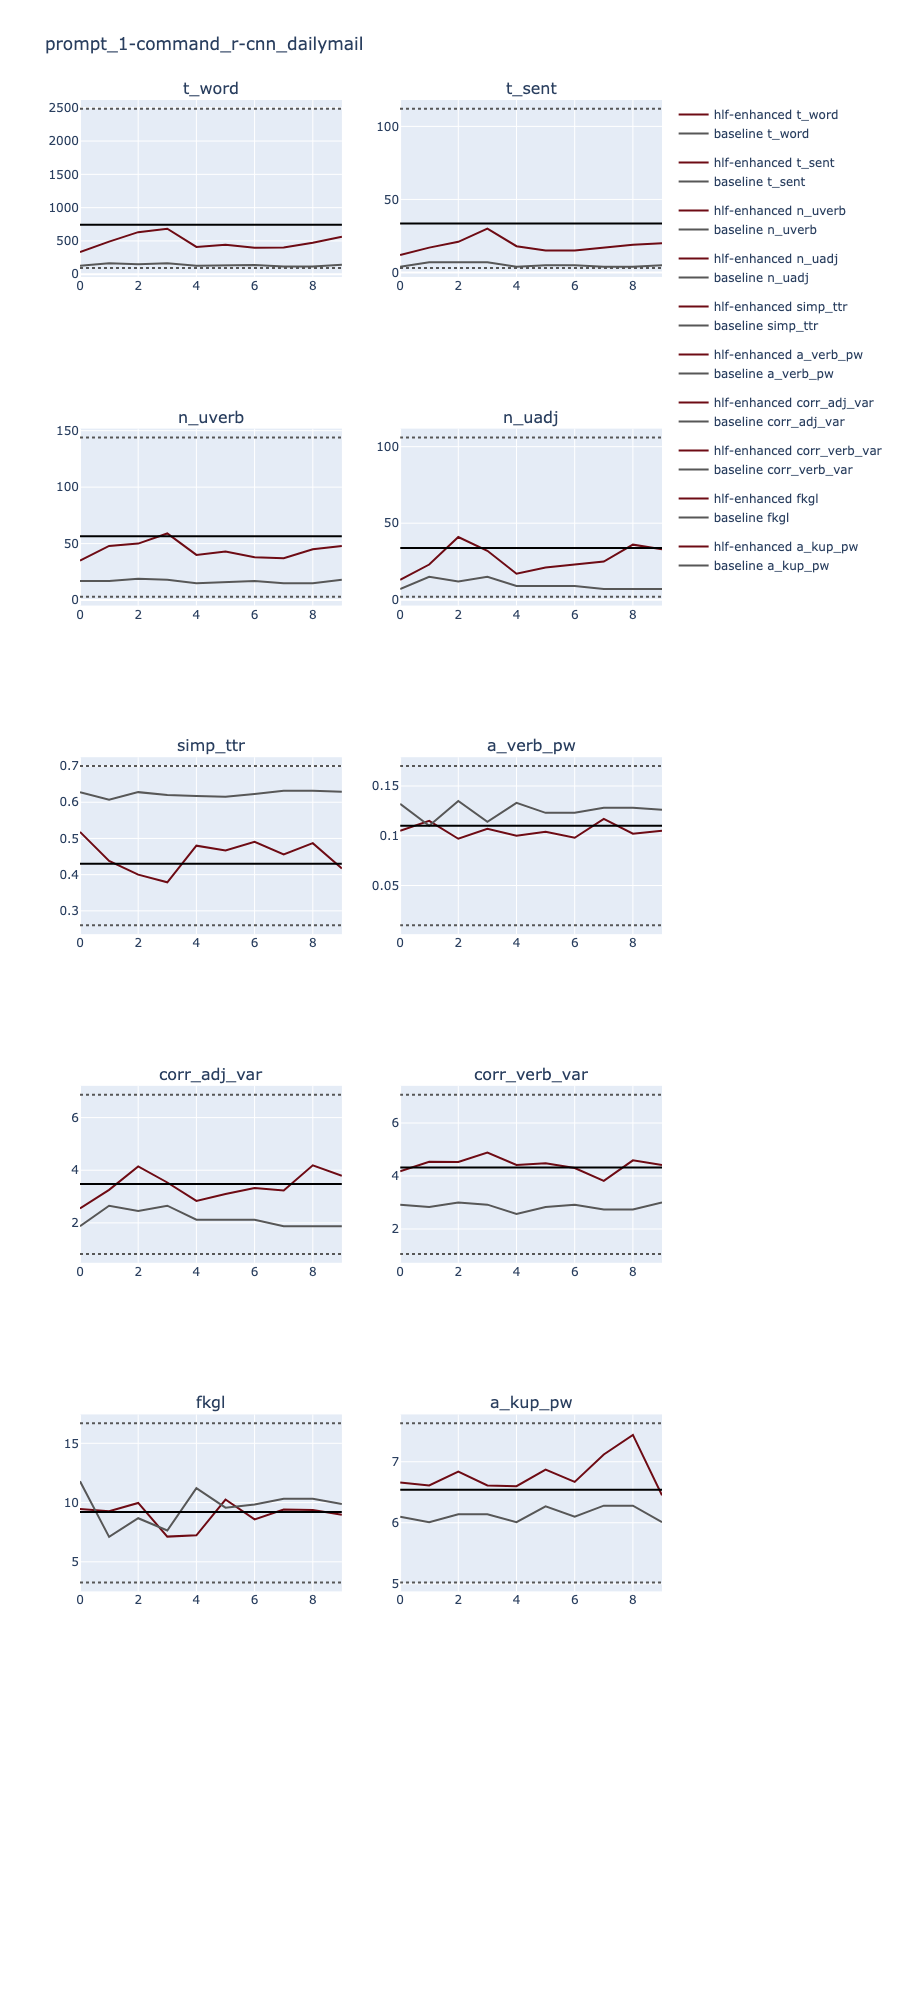
\includegraphics[width=\textwidth,height=0.9\textheight,scale=1]{plots/prompt_1/prompt_1-command_r-cnn_dailymail/prompt_1-command_r-cnn_dailymail.png}
    \caption{Command R on CNN Corpus\\Prompt Without Examples}\label{fig:command_r-prompt1-cnn}
\end{figure*}
\begin{figure*}[ht]
    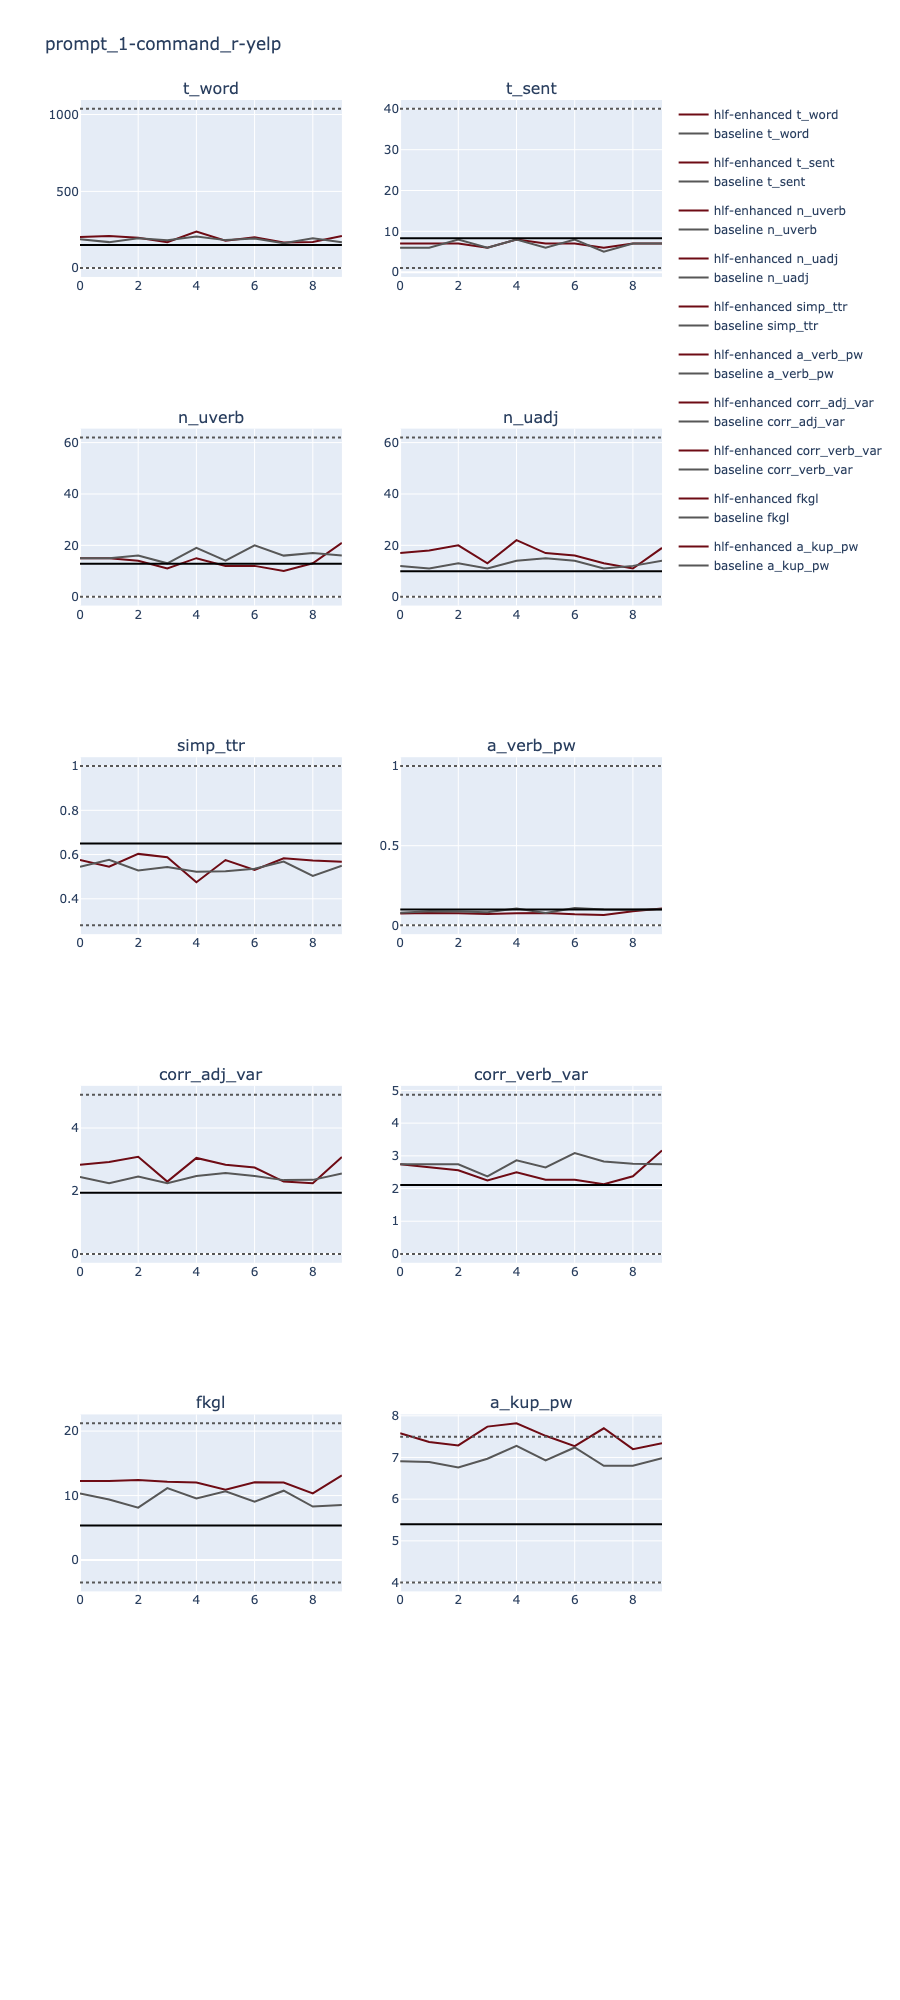
\includegraphics[width=\textwidth,height=0.9\textheight,scale=1]{plots/prompt_1/prompt_1-command_r-yelp/prompt_1-command_r-yelp.png}
    \caption{Command R on Yelp Corpus\\Prompt Without Examples}\label{fig:command_r-prompt1-yelp}
\end{figure*}
\begin{figure*}[ht]
    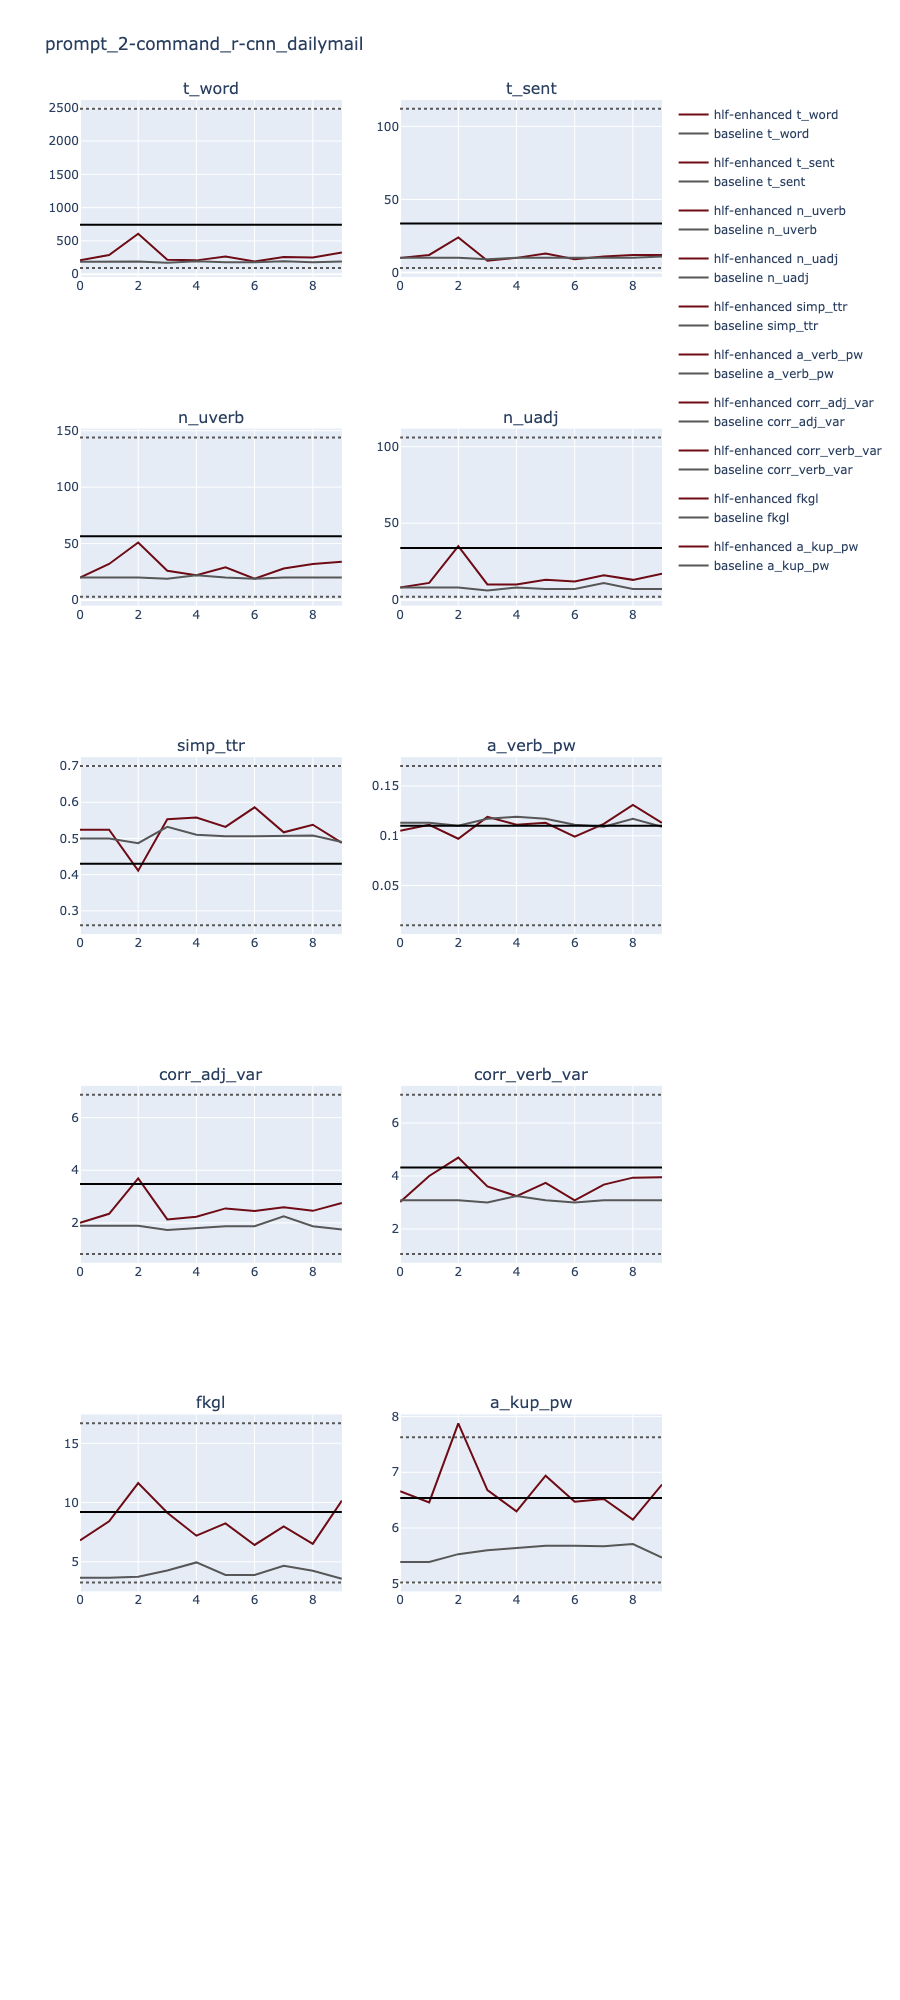
\includegraphics[width=\textwidth,height=0.9\textheight,scale=1]{plots/prompt_2/prompt_2-command_r-cnn_dailymail/prompt_2-command_r-cnn_dailymail.png}
    \caption{Command R on CNN Corpus\\Prompt With Examples\\Extraneous Input}\label{fig:command_r-prompt2-cnn}
\end{figure*}
\begin{figure*}[ht]
    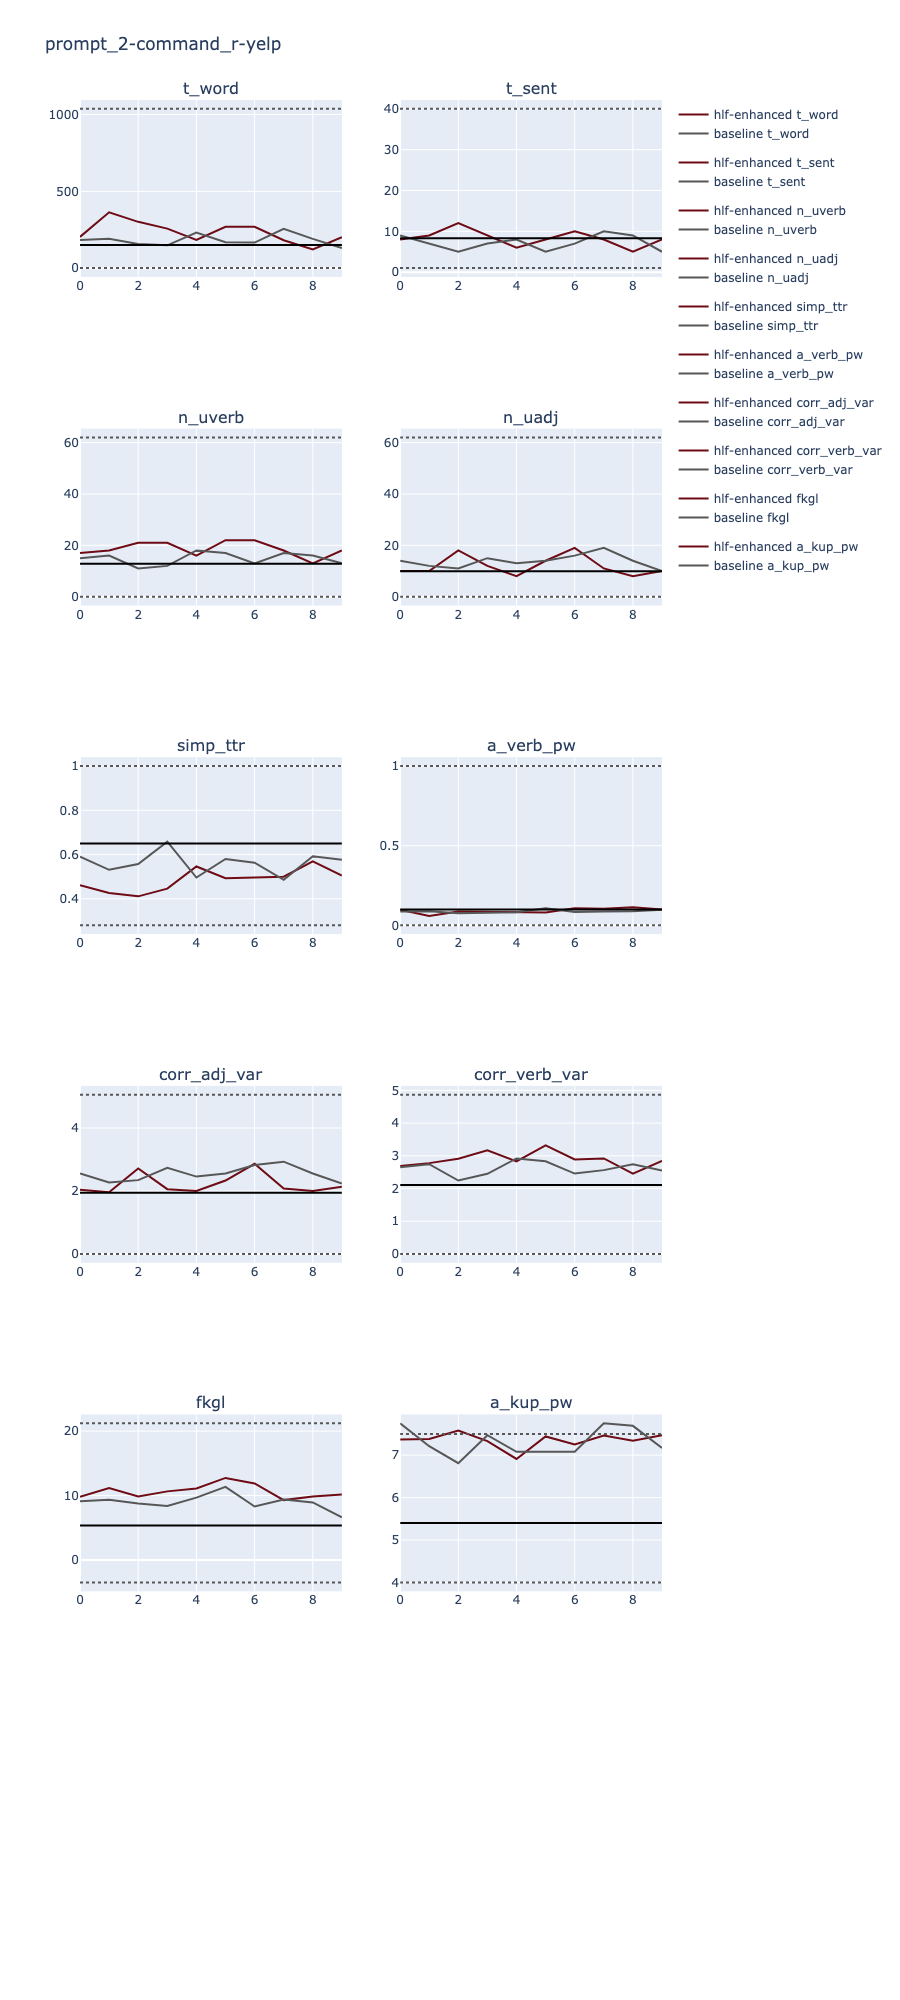
\includegraphics[width=\textwidth,height=0.9\textheight,scale=1]{plots/prompt_2/prompt_2-command_r-yelp/prompt_2-command_r-yelp.png}
    \caption{Command R on Yelp Corpus\\Prompt With Examples\\Extraneous Input}\label{fig:command_r-prompt2-yelp}
\end{figure*}
\begin{figure*}[ht]
    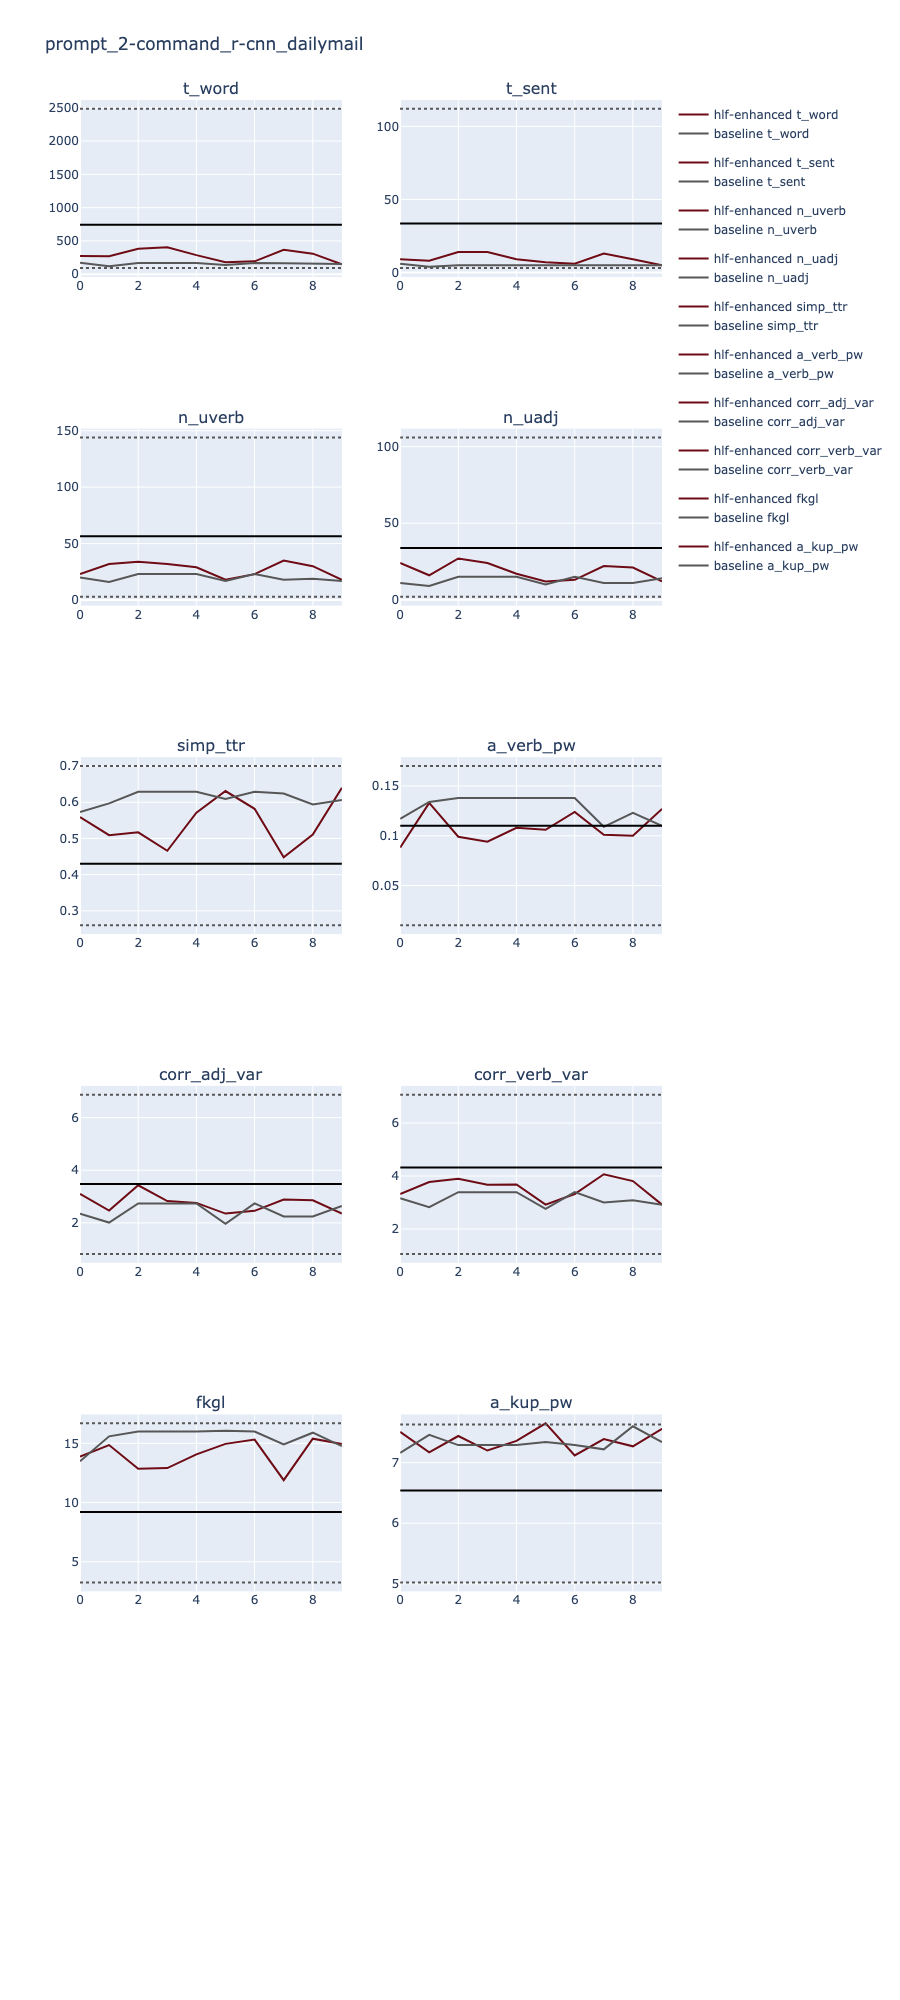
\includegraphics[width=\textwidth,height=0.9\textheight,scale=1]{plots/prompt_2_ifd/prompt_2-command_r-cnn_dailymail/prompt_2-command_r-cnn_dailymail.png}
    \caption{Command R on CNN Corpus\\Prompt With Examples\\Input from Corpus}\label{fig:command_r-prompt2-cnn-ifd}
\end{figure*}
\begin{figure*}[ht]
    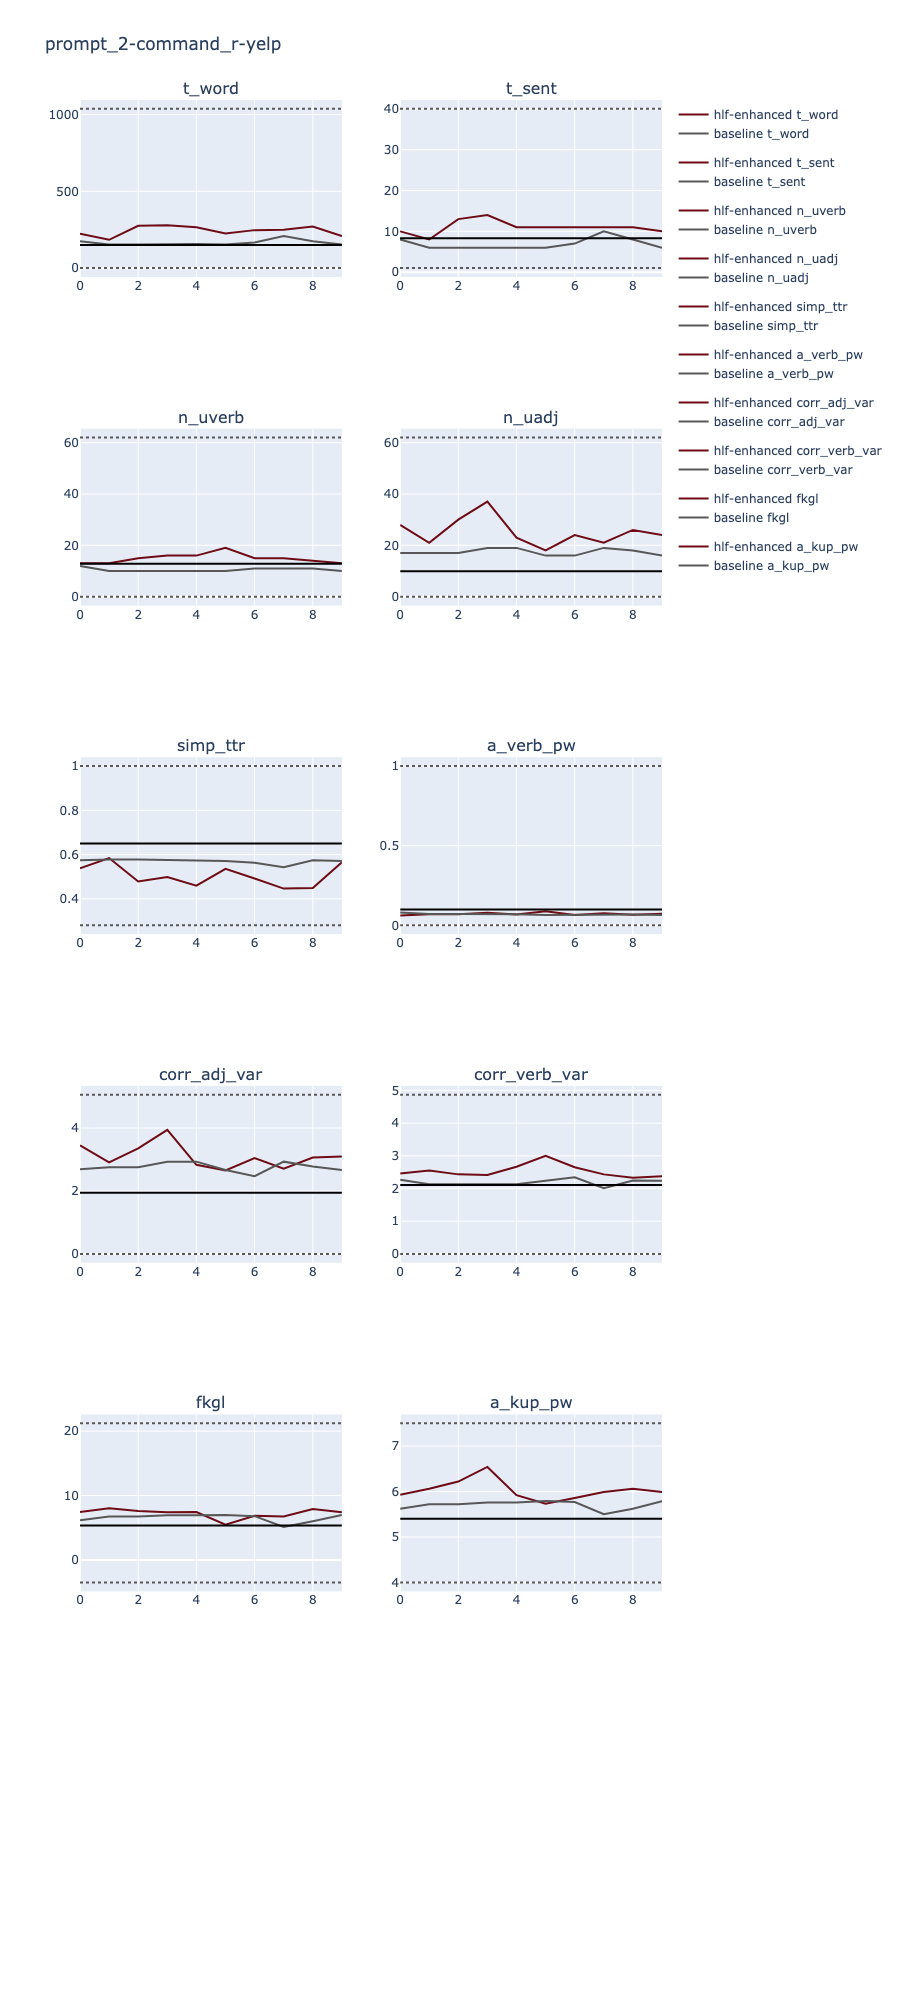
\includegraphics[width=\textwidth,height=0.9\textheight,scale=1]{plots/prompt_2_ifd/prompt_2-command_r-yelp/prompt_2-command_r-yelp.png}
    \caption{Command R on Yelp Corpus\\Prompt With Examples\\Input from Corpus}\label{fig:command_r-prompt2-yelp-ifd}
\end{figure*}

\Cref{fig:command_r-prompt1-cnn,fig:command_r-prompt1-yelp,fig:command_r-prompt2-cnn,fig:command_r-prompt2-yelp,fig:command_r-prompt2-cnn-ifd,fig:command_r-prompt2-yelp-ifd}
show the experiment results for the Claude 3 Opus large language model.

\end{document}